%% 2021/01/16 2:39、Antonio J. Peña <antonio.pena@bsc.es> wrote;
%%
%% Hi folks,
%%
%% This is a friendly reminder. Submission site has just opened
%% today. Deadline: Feb. 15.
%%
%% Submission site: https://www.editorialmanager.com/PARCO/default.aspx
%%
%% Please make sure  you select “VSI:EuroMPI/USA 2020” as the article type.
%%
%% A few more remarks:
%%  - Please remember to include at the very least 30% new substantial
%% contribution. If you need space, just remove some text and refer to
%% the original paper (which you should do anyway to explain the
%% differences between both papers)
%%  - Try to stick to 14 pages (double-column format)
%%  - It is strongly advised to slightly change the title to avoid
%% confusion, since in the end these will be two different papers
%%
%% Please let us know any concerns.
%%

%% On 19/11/20 11:54, Mohror, Kathryn wrote:
%% Hello everyone!
%%
%% Thank you for your interest in submitting an extension of your
%% EuroMPI/USA 2020 work into a special issue of the Journal of Parallel
%% Computing. The journal has accepted our special issue proposal, so now
%% it’s time to get to work!
%%
%% Papers submitted to the journal must have substantive additional
%% contribution of 30-40\% over previously published papers, including
%% the EuroMPI/USA 2020 conference version. It is not sufficient to
%% simply add a long related work section or more discussion. The papers
%% must have a decent update all over and have new content (e.g.,
%% results, algorithms) over the original.
%%
%% Paper submission guidelines:
%% https://www.elsevier.com/journals/parallel-computing/0167-8191/guide-for-authors
%% Paper submission portal opens: January 14, 2021
%% Paper submission portal closes: February 15, 2021
%%
%% Please let us know of your questions or concerns on this.
%%
%% Best regards,
%% Kathryn Mohror and Toni Pena

\documentclass[preprint,5p,times]{elsarticle}
%\documentclass[review,5p,times]{elsarticle}
%\documentclass[doubleblind,5p,times]{elsarticle}

\bibliographystyle{model1-num-names}
%\bibliographystyle{model2-names.bst}\biboptions{authoryear}

\usepackage{graphicx}
\usepackage{balance}
\usepackage{url}
\usepackage{paralist}
\usepackage[inline]{enumitem}
\setlist[enumerate,1]{label=\bf{\alph*)}}
%
\usepackage{todonotes}%
\usepackage{color}%
\usepackage{underscore}%
%
\def\myquote#1{{\it #1}}
\long\def\comment#1{}
%
%%%%%%%%%%%%%%%%%%%%%%%%%%
\begin{document}

\title{An International Survey on MPI Users}

%%\tnotetext[tnote]{This is a questionnaire survey report on
%%  international MPI users}

\author[1]{Atsushi Hori\corref{cor}}\ead{ahori@riken.jp}
\author[2]{Emmanuel Jeannot}\ead{emmanuel.jeannot@inria.fr}
\author[3]{George Bosilca}\ead{bosilca@icl.utk.edu}
\author[1]{Takahiro Ogura}\ead{t-ogura@riken.jp}
\author[1]{Balazs Gerofi}\ead{bgerofi@riken.jp}
\author[1]{Jie Yin}\ead{jie.yin@riken.jp}
\author[1]{Yutaka Ishikawa}\ead{yutaka.ishikawa@riken.jp}

\affiliation[1]{organization={Riken Center for Computational Science},
  addressline={7-1-26 Minatojima-minami-machi, Chuo-ku},
  city={Kobe},
  postcode={650-0047},
  country={Japan}
}
\affiliation[2]{organization={INRIA Bordeaux Sud-Ouest},
  addressline={200, Avenue de la Vielle Tour},
  city={Talence},
  postcode={33405},
  country={France}
}
\affiliation[3]{organization={Innovative Computing Laboratory,
    University of Tennessee},
  addressline={Suite 203 Claxton, 1122 Volunteer Blvd, },
  city={Knoxville},
  postcode={37996},
  country={USA}
}

\begin{abstract}
  The Message Passing Interface (MPI) plays a crucial part in the
  parallel computing ecosystem, a driving force behind many of the
  high-performance computing (HPC) successes. To maintain its relevance
  to the user community---and in particular to the growing HPC community
  at large---the MPI standard needs to identify and understand the MPI
  users' concerns and expectations, and adapts
  accordingly to continue to efficiently bridge the gap between users and hardware. This questionnaire survey was conducted starting from February
  2019 by using two online questionnaire frameworks, and more than 850
  answers from 42 countries has gathered at the time of this writing.
  % There are some predecessors of this kind of survey.
  Some of preceding work in surveying MPI uses are questionnaire surveys
  like ours, while others are conducted either by analyzing MPI programs
  to reveal static behavior or by analyzing dynamic runtime behavior of
  MPI jobs by using profiling tools. Our survey is different from the
  other questionnaire survey in terms of geographically wide-spread and
  the much larger number of participants. As a result it is possible to
  illustrate the current status of MPI users more accurately and with a
  wider geographical distribution. In this report, we will show some
  interesting findings, comparing the results with preceding studies
  when possible.
\end{abstract}

\begin{keyword}
  \MSC[2020]{68-02} \sep Message Passing Interface (MPI) \sep survey
\end{keyword}

\maketitle

\section{Background}

Existing studies on MPI uses are focused on a restricted target
domain, such as the Exascale Computing Project (ECP)~\cite{ECP} study
conducted in 2017~\cite{ECP-survey} that focused
on MPI usage in the
context of ECP applications; and/or are generally geographically
constrained to a single laboratory, funding agency or at best,
country. As such they provide sporadic, disconnected views on the real
uses of MPI across the world.
%
Interestingly enough, and mostly by coincidence, simultaneously with
the ECP study another survey was conducted in Japan targeting
HPCI~\cite{HPCI} users which included several questions asking about
MPI~\cite{hpci-user-survey}.  HPCI is an infrastructure for HPC users
in Japan connecting major supercomputers owned by universities and
governmental research institutes. If both questionnaire surveys would
have the same questions, we could have compared the answers to reveal
the differences between US and Japan MPI user
communities. Unfortunately, a single question was similar in both
studies, limiting the correlations between the two surveys.

These studies highlighted the need to conduct a larger, more comprehensive,
study, reaching across many diverse community of MPI users, and therefore
inspired our effort. Unlike it's predecessors we shifted the study's focus from
the high-end HPC community, and targeted a wider audience and involved a larger
spectrum of geographically distinct users. Since MPI has been a widely used
vehicle for high-performance computing for decades, this larger-scale
questionnaire survey would be beneficial not only for deciding the future
direction of MPI, but also for understanding the feature differences of MPI
users among countries and/or regions of the world.

Our team started to conduct such a study as a project at
JLESC~\cite{JLESC} which is an international research collaboration
framework. The international nature of this survey matches the concept
of JLESC. Co-authors are a member of JLESC and responsible for the
country and/or region where they belong. For the design of the questionnaire,
we consulted two social scientists, Prof. Marshall Scott Poole at
Illinois Univ., and Prof. Iftekhar Ahmed at Univ. of North Texas,
participating JLESC workshops to investigate how researchers can
collaborate in the JLESC framework.

\begin{table}[htb]%
  \begin{center}%
    \caption{Comparison of ECP and HPCI
      Surveys}\label{tab:comparison}%
    \begin{tabular}{c|ccc}%
      \hline
      & ECP & HPCI & ours \\
      \hline
      \hline
      Concern & {\small MPI usage in} & Computing & MPI \\
              & Exascale & Environment & {\small (w/o MPI-IO)} \\
              & Computing & & \\
      \hline%
      Target & USA & Japan & World \\
      \hline
      \#Questions & 64 (max) & 75 (max) & 30 \\
      \hline
      \#Participants & 77 & 105 & 851 \\
      \hline
    \end{tabular}%
  \end{center}%
\end{table}%

To give an order of comparison with preceding studies, our MPI
International Survey, ECP survey, and HPCI survey are summarized in
Table~\ref{tab:comparison}.

\comment{
  The major differences
  between our survey and the others are;
  \begin{description}
  \item[Geographic Target]\mbox{}\\
    The ECP survey targeted ECP members who are leading researchers and
    application developers in the US. The ECP survey targeted high-end
    users. Whereas our survey targets all MPI users from novices to experts.
  \item[Number of participants]\mbox{}\\
    The number of participants of the ECP survey is 77. Because of the wider
    target of our survey, in terms of the scope of MPI expertise of
    participants on a global scale, the expected number of answers would
    be larger than those of preceding surveys.
  \item[Number of questions]\mbox{}\\
    The number of questions in our survey is 30 which is much
    smaller than those of the other surveys.
  \end{description}
}

\section{Related Work}

The existing MPI-related surveys can be categorized in three survey classes;
%
questionnaire survey asking MPI users questions specifically crafted toward a
target goal ({\em Q}) and reflecting more the human understanding or knowledge of MPI capabilities,
%
application-oriented statistical surveys statically analyzing MPI programs and
classifying occurrences of MPI calls ({\em S}),
%
and application-oriented statistical surveys analyzing MPI applications behavior
at runtime by using a profiling tool ({\em R}).

Our survey and the ECP survey are examples of the {\em Q} category, and highlight, as mentioned above, the user understanding of MPI capabilities and knowledge of MPI features. They can more easily identify what new MPI features are become known by the users community, well before they start appearing in MPI applications.
% while \cite{https://doi.org/10.1002/cpe.5901} can be categorized as {\em S}, and \cite{8665758,10.1007/978-3-319-58667-0-12} are of class {\em R}.

In the {\em S} category, \cite{10.1145/3295500.3356176} statically investigated
110 open-source MPI programs. \cite{cpe-5901}
investigated 14 MPI programs chosen from the ECP Proxy Applications Suite
2.0~\cite{osti-1482870}. They offer a pragmatic view on the usage patterns of
MPI function in existing applications, and can serve as an indicator of what MPI
features translates into real usages.

In the {\em R} category, \cite{8665758} collected and
analyzed the runtime behavior by running more than 100K MPI
jobs, with a smaller but still significantly distinct number of different applications. \cite{10.1007/978-3-319-58667-0-12} takes a similar approach, but focuses on HPC applications and analyzed the behavior of DOE
Mini-apps based on the trace data which DOE made public. It is interesting to note that the target community for these 2 studies is significantly different, the second one looking at applications developed by a user community more inclined to use advanced features of MPI.

The target of the questionnaire surveys are MPI users, the target of
{\em S} is MPI programs, and the target of {\em R} is MPI jobs. In spite of
these target differences, we dare to compare some results of those
non-questionnaire-based surveys and ours in the
following sections as appropriate.

\section{Survey}

\subsection*{Design}
%
The social scientists suggested that the number of questions must be limited
around 30, to keep participants engaged and not to loose their concentration and
focus. This number is significantly smaller that those of ECP and HPCI surveys,
forcing us to restrict the scope of the questions, and focus on few, critical
aspects to the future of the MPI effort. As an example, we deliberately excluded
some topics, such as MPI-IO, and instead focused on MPI communications.
%\todo{I don't understand the next sentence}
%Additionally, we designed the questionnaire for participants can easily answer
%questions as much as possible, and the questions to force participants doing
%some work, such as counting the lines of code, are eliminated.
% AH rewrote, Jan 29
We designed the questionnaire so that participants can answer questions
as easy as possible, and the questions to force participants doing
some extra work to answer the questions, such as counting the lines of
code of their programs, are eliminated. 

Similarly to the ECP questionnaire, we initially started with Google Forms to
develop ours. Later in our project, and mostly for geopolitical reasons, we
replicated the same questionnaire using Microsoft Forms for those who cannot
access Google Forms. All graphs in this paper were generated using the
aggregated data from both forms (Google and Microsoft) exported using a CVS
format, and then manipulated using statistical tools developed in Python and R.

The draft questionnaire was tested and validated by several active members of
the MPI standardization body, as well as researchers from Inria and Riken Center
for Computational Science (R-CCS).
% We also interviewed with Dr. Kento Sato at R-CCS.
The questionnaire was was available online and receiving answers from February
17, 2019 until recently. In fact, the two forms remain open to additional
answers, but taking in account the rate of the contributions we do not expect
the outcome to drastically change.
%  The most recent answer was obtained at June 22, 2020.
All questions, their choices, and abbreviations of the choices used in
this report are listed in ~\ref{app:questions}.

\subsection*{Distribution}

\begin{figure}[htb]
  \begin{center}
    %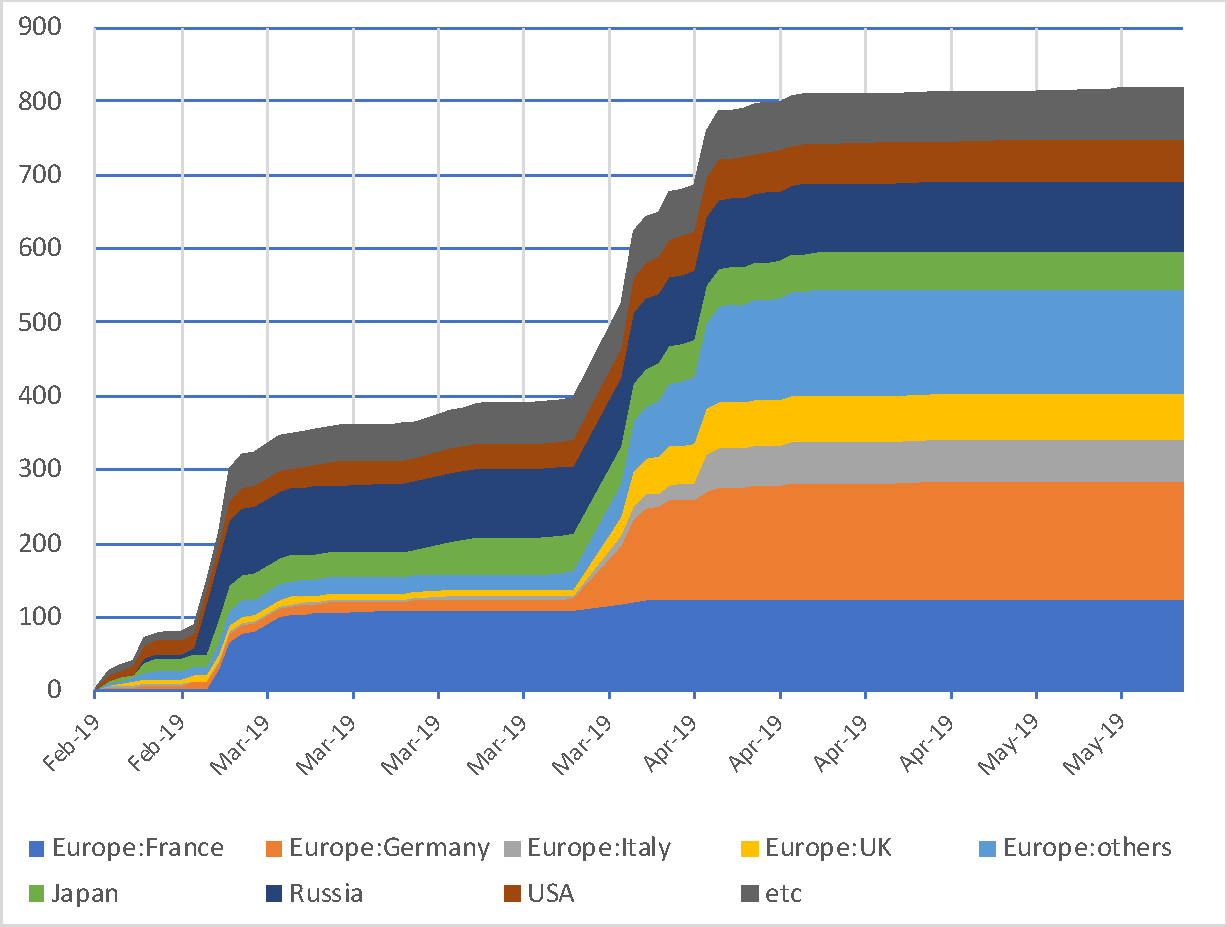
\includegraphics[width=8cm]{Figs/TimeSeries-Zoom.pdf}
    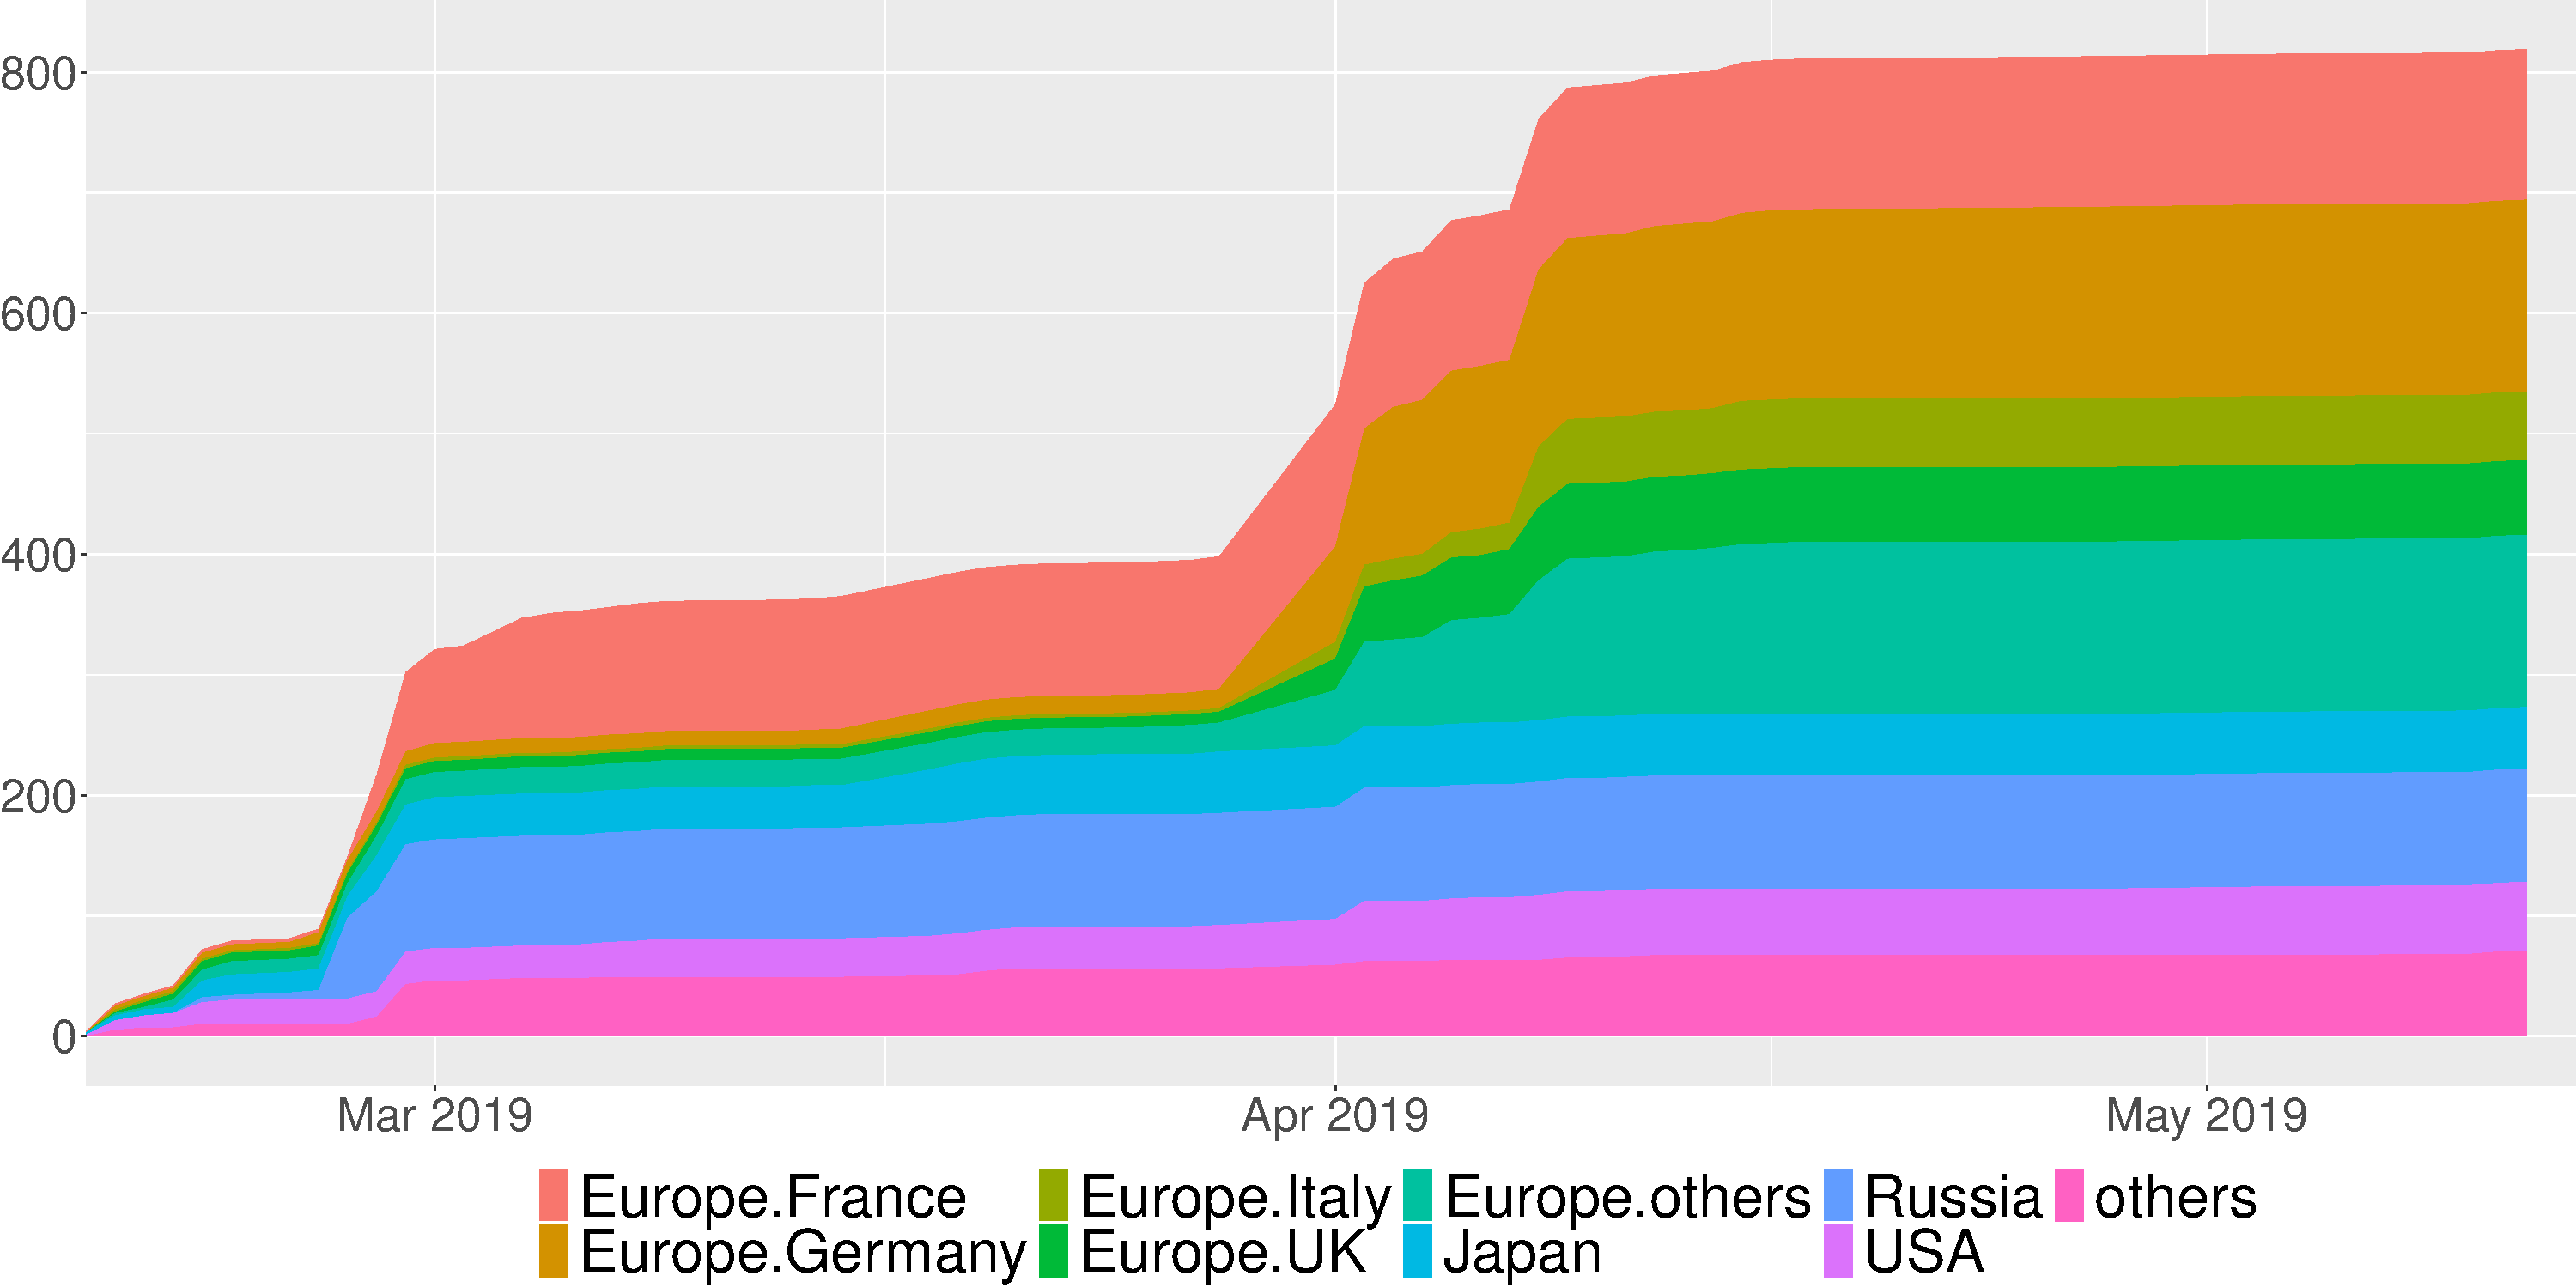
\includegraphics[width=8.7cm]{R-scripts/TimeSeries.pdf}
    \caption{Time series in first 90 days}
    \label{fig:time-series}
  \end{center}
\end{figure}

One of the first questions we had to ask was hot to reach a largely
international community of researchers and users, quickly and efficiently while hoping for a significant contribution.
%
The survey was initially announced via several major mailing lists in the
community such as {\tt hpc-announce@mcs.anl.gov}, but the contributions were
extremely slow to arrive. In order to improve participation, we decided to
approach the problem more locally and reached out to different collaborators and
asked them to locally distribute the questionnaire inside their institutions,
via their own distribution process (mailing list, forums, or different form of
social platforms). As highlighted in Fig.~\ref{fig:time-series}, more localized
means of distribution were highly beneficial, each one of the steps in the
figure corresponding to a new distribution campaign to a new set of
institutions.

% Soon after started, we realized the number of responses was not as many as we
% expected. Hence, we asked people who can reach local regions. Distribution
% using local mailing-lists worked much better than that of major mailing lists.
% Fig.~\ref{fig:time-series} shows the transition of the number of answers at
% the first three months. As shown there are several steps and those steps came
% out after asking local distribution.

This local distribution strategy worked well on some regions but
did not work universally. Table~\ref{tab:countries} shows the number
of participants of top 11 countries (all countries are listed in
\ref{app:countries}).
Comparing with Table~\ref{tab:top500-share} listing the top 10
countries in the performance share in the Top500~\cite{Top500}, the
three major countries, USA, China and Japan in Top500, are not even in
the top 5 in our survey. Especially China has only 18 participants
including
Taiwan (2). We tried to increase the number of participants of those
countries as much as we could, making and distributing fliers at
several conferences, with little positive outcome. While the root cause is still unclear, this pinpoints to the need for alternative distribution schemes, especially in these locations.
%  Possibly because we could not reach the right influencing person to ask, or
%  maybe because of % nationalities.

\subsection*{Major contributors}

For the remaining of this report, countries or regions having more than 50
participants are called {\bf major contributors} and are the
objects of cross-tab analysis. Those are
Germany, France, Russia, UK, Japan, USA, Italy and
the rest of European countries.
There is a trade-off between the number of participants of
each major country
and the number of the major contributors in the cross-tab analysis. The
threshold of 50 participants was selected to balance this trade-off
but this is not our intention of saying 50 is enough. Hence, some
cross-tab analysis may not be reliable enough.
It should be noted that we asked the
workplaces in past 5 years, not asking nationalities.
%
\begin{table}%
\begin{center}%
\caption{Top 11 Countries of Participants}\label{tab:countries}%
\begin{tabular}{c|l|r|r}%
  \hline%
  \# & Country & \#Ans & [\%] \\%
  \hline%
  1 & Germany 	& 159 & 18.7 \\%
  2 & France 	& 125 & 14.7 \\%
  3 & Russia 	& 94  & 11.1 \\%
  4 & UK 		& 67  &  7.9 \\%
  5 & Japan 	& 64  &  7.5 \\%
  6 & USA 	& 58  &  6.8 \\%
  7 & Italy 	& 57  &  6.6 \\%
  \hline%
  8 & Switzerland & 40  &  5.8 \\%
  9 & South Korea & 27  &  3.2 \\%
  10 & Austria 	& 26  &  3.1 \\%
  11 & China (incl. Taiwan) & 18 & 2.1 \\%
  \hline%
  \multicolumn{4}{c}{42 countries, 851 participants} \\%
\end{tabular}%

\caption{Top500 Performance Share (Nov. 2020)}\label{tab:top500-share}%
  \begin{tabular}{c|l|r}%
    \hline%
    \# & Country & [\%] \\%
    \hline%
    1  & USA 	  & 27.5 \\%
    2  & China 	  & 23.3 \\%
    3  & Japan 	  & 24.4 \\%
    4  & Germany  &  5.4 \\%
    5  & France	  &  3.7 \\%
    6  & Italy	  &  3.2 \\%
    7  & UK	  &  1.4 \\%
    8  & Canada	  &  1.1 \\%
    9  & Netherlands  & 1.0 \\%
    10 & Switzerland  & 1.0 \\%
    \hline%
  \end{tabular}%
\end{center}%
\end{table}%

\subsection*{Participants' profile}

Fig.~\ref{fig:occupations} shows the graph of Q1 asking participants'
occupation. As shown, roughly 80\% of participants are working at
universities or governmental research institutes.
%
\begin{figure}[htb]
  \begin{center}
    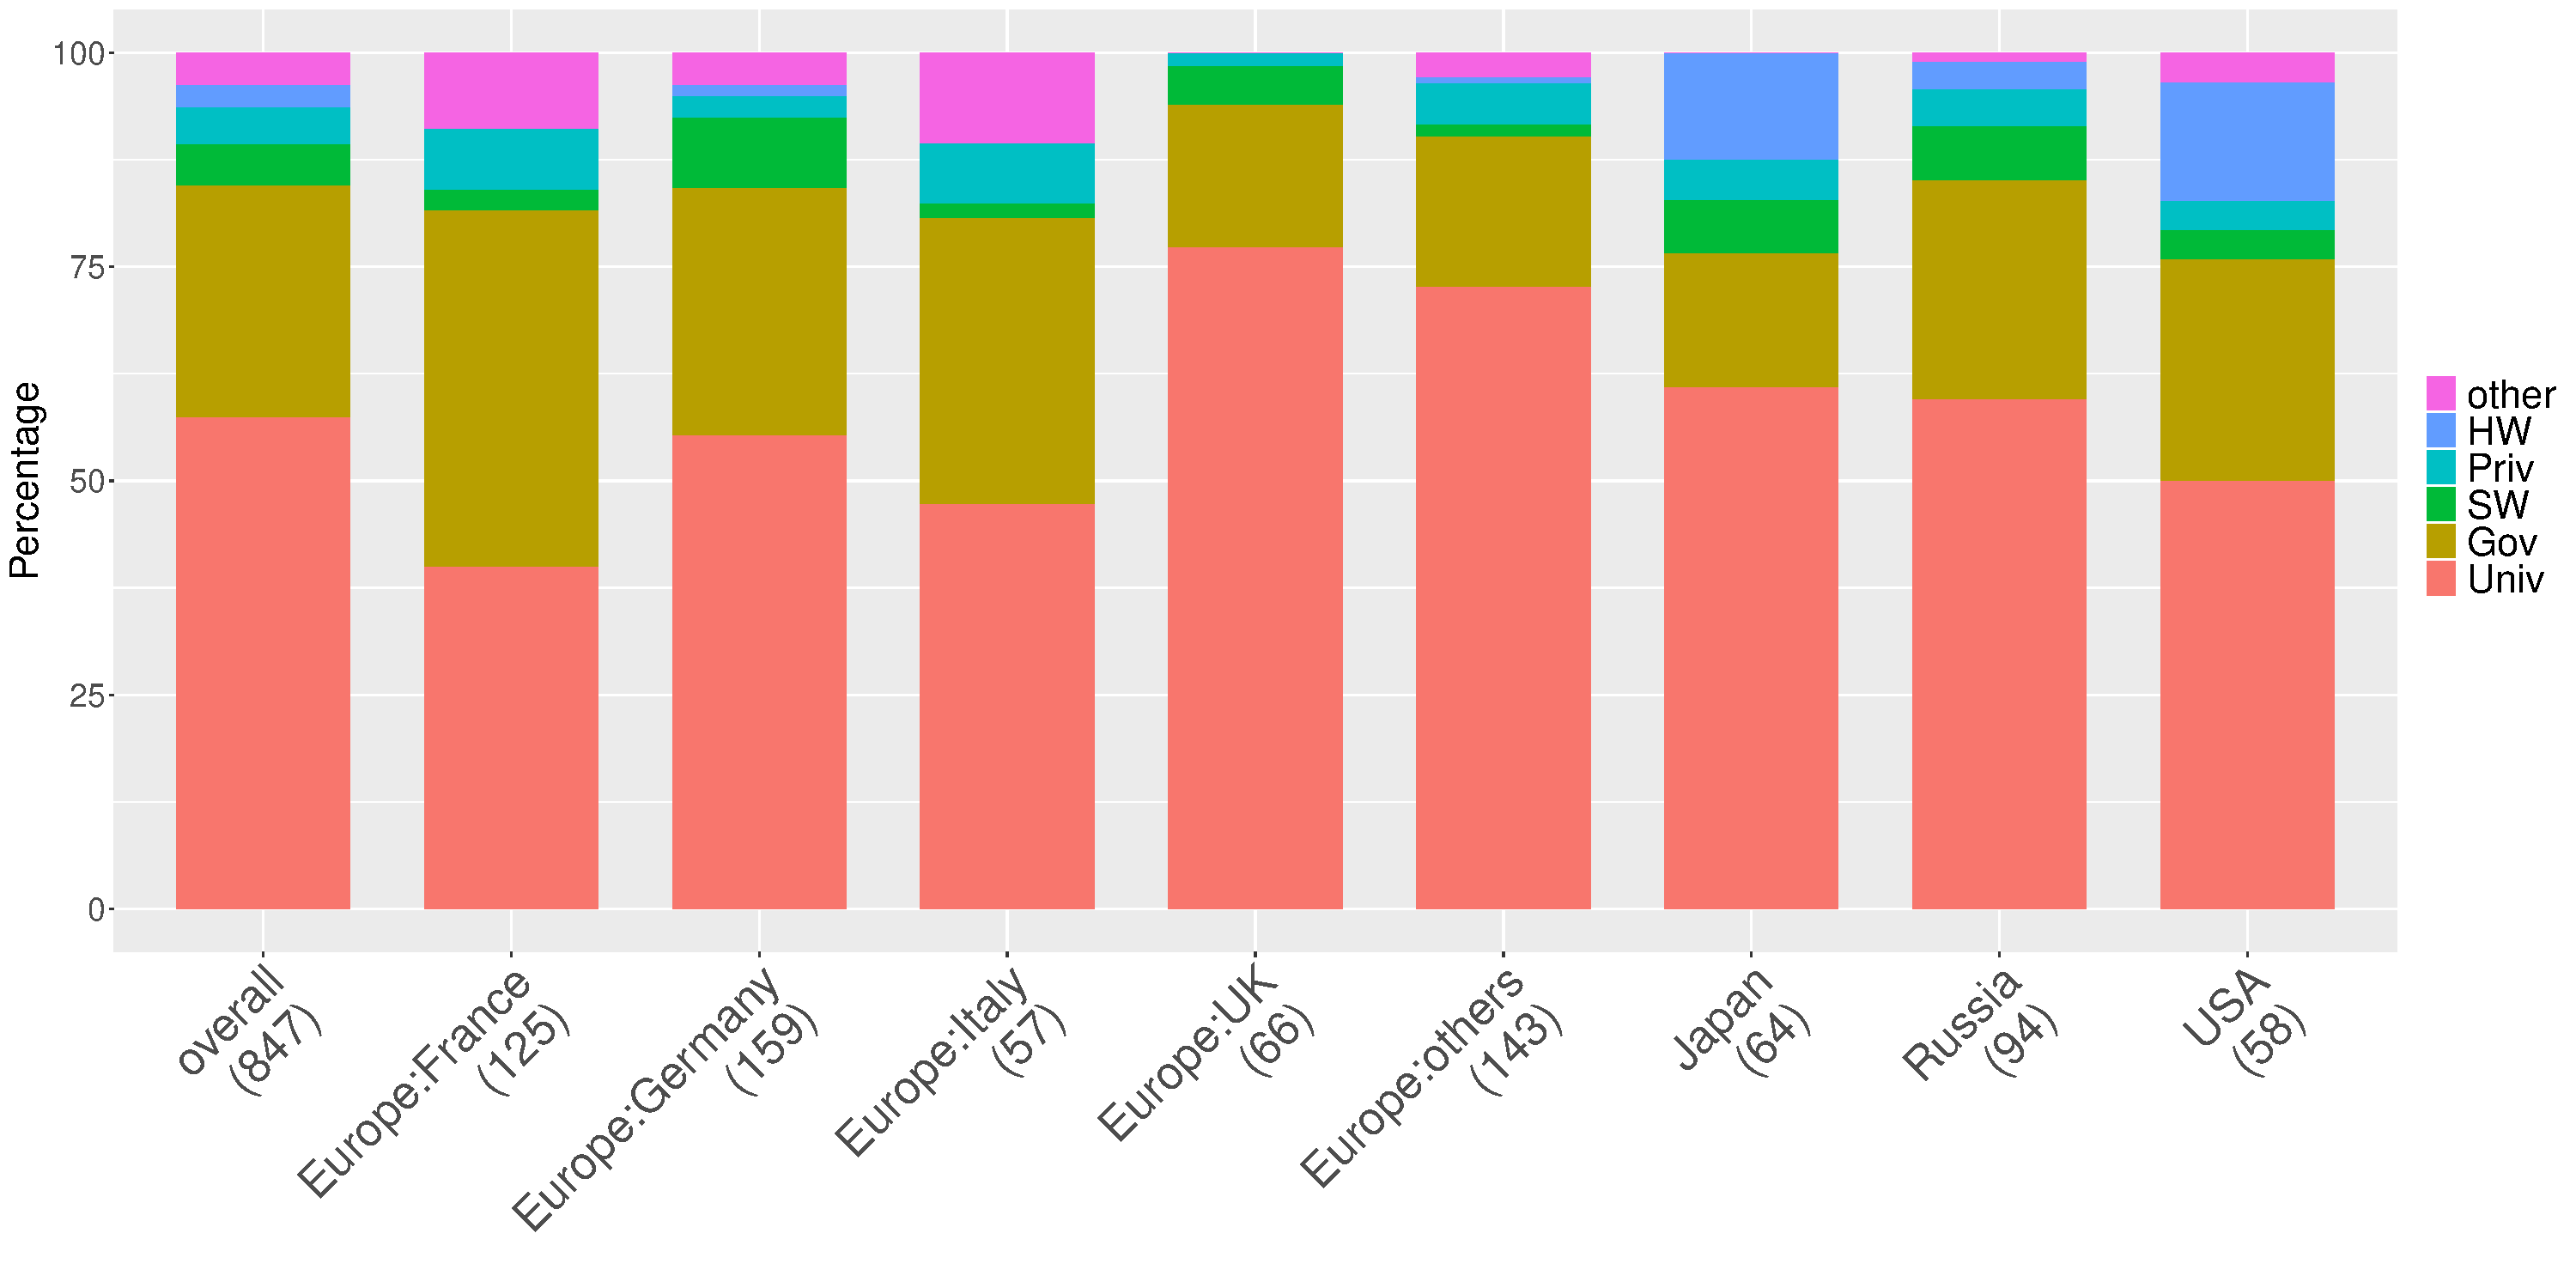
\includegraphics[width=8.7cm]{R-scripts/Q1.pdf}
    \caption{Q1: Occupations {\it(single)}}
    \label{fig:occupations}
  \end{center}
\end{figure}

Fig.~\ref{fig:working-fields} shows the result of asking \myquote{Which
fields are you mostly working in?}. Generally speaking, most
participants are working on numerical applications and/or
libraries. In Japan and US, the percentages of parallel languages and
OS/runtimes are higher than the other countries and regions.

\begin{figure}[htb]
  \begin{center}
    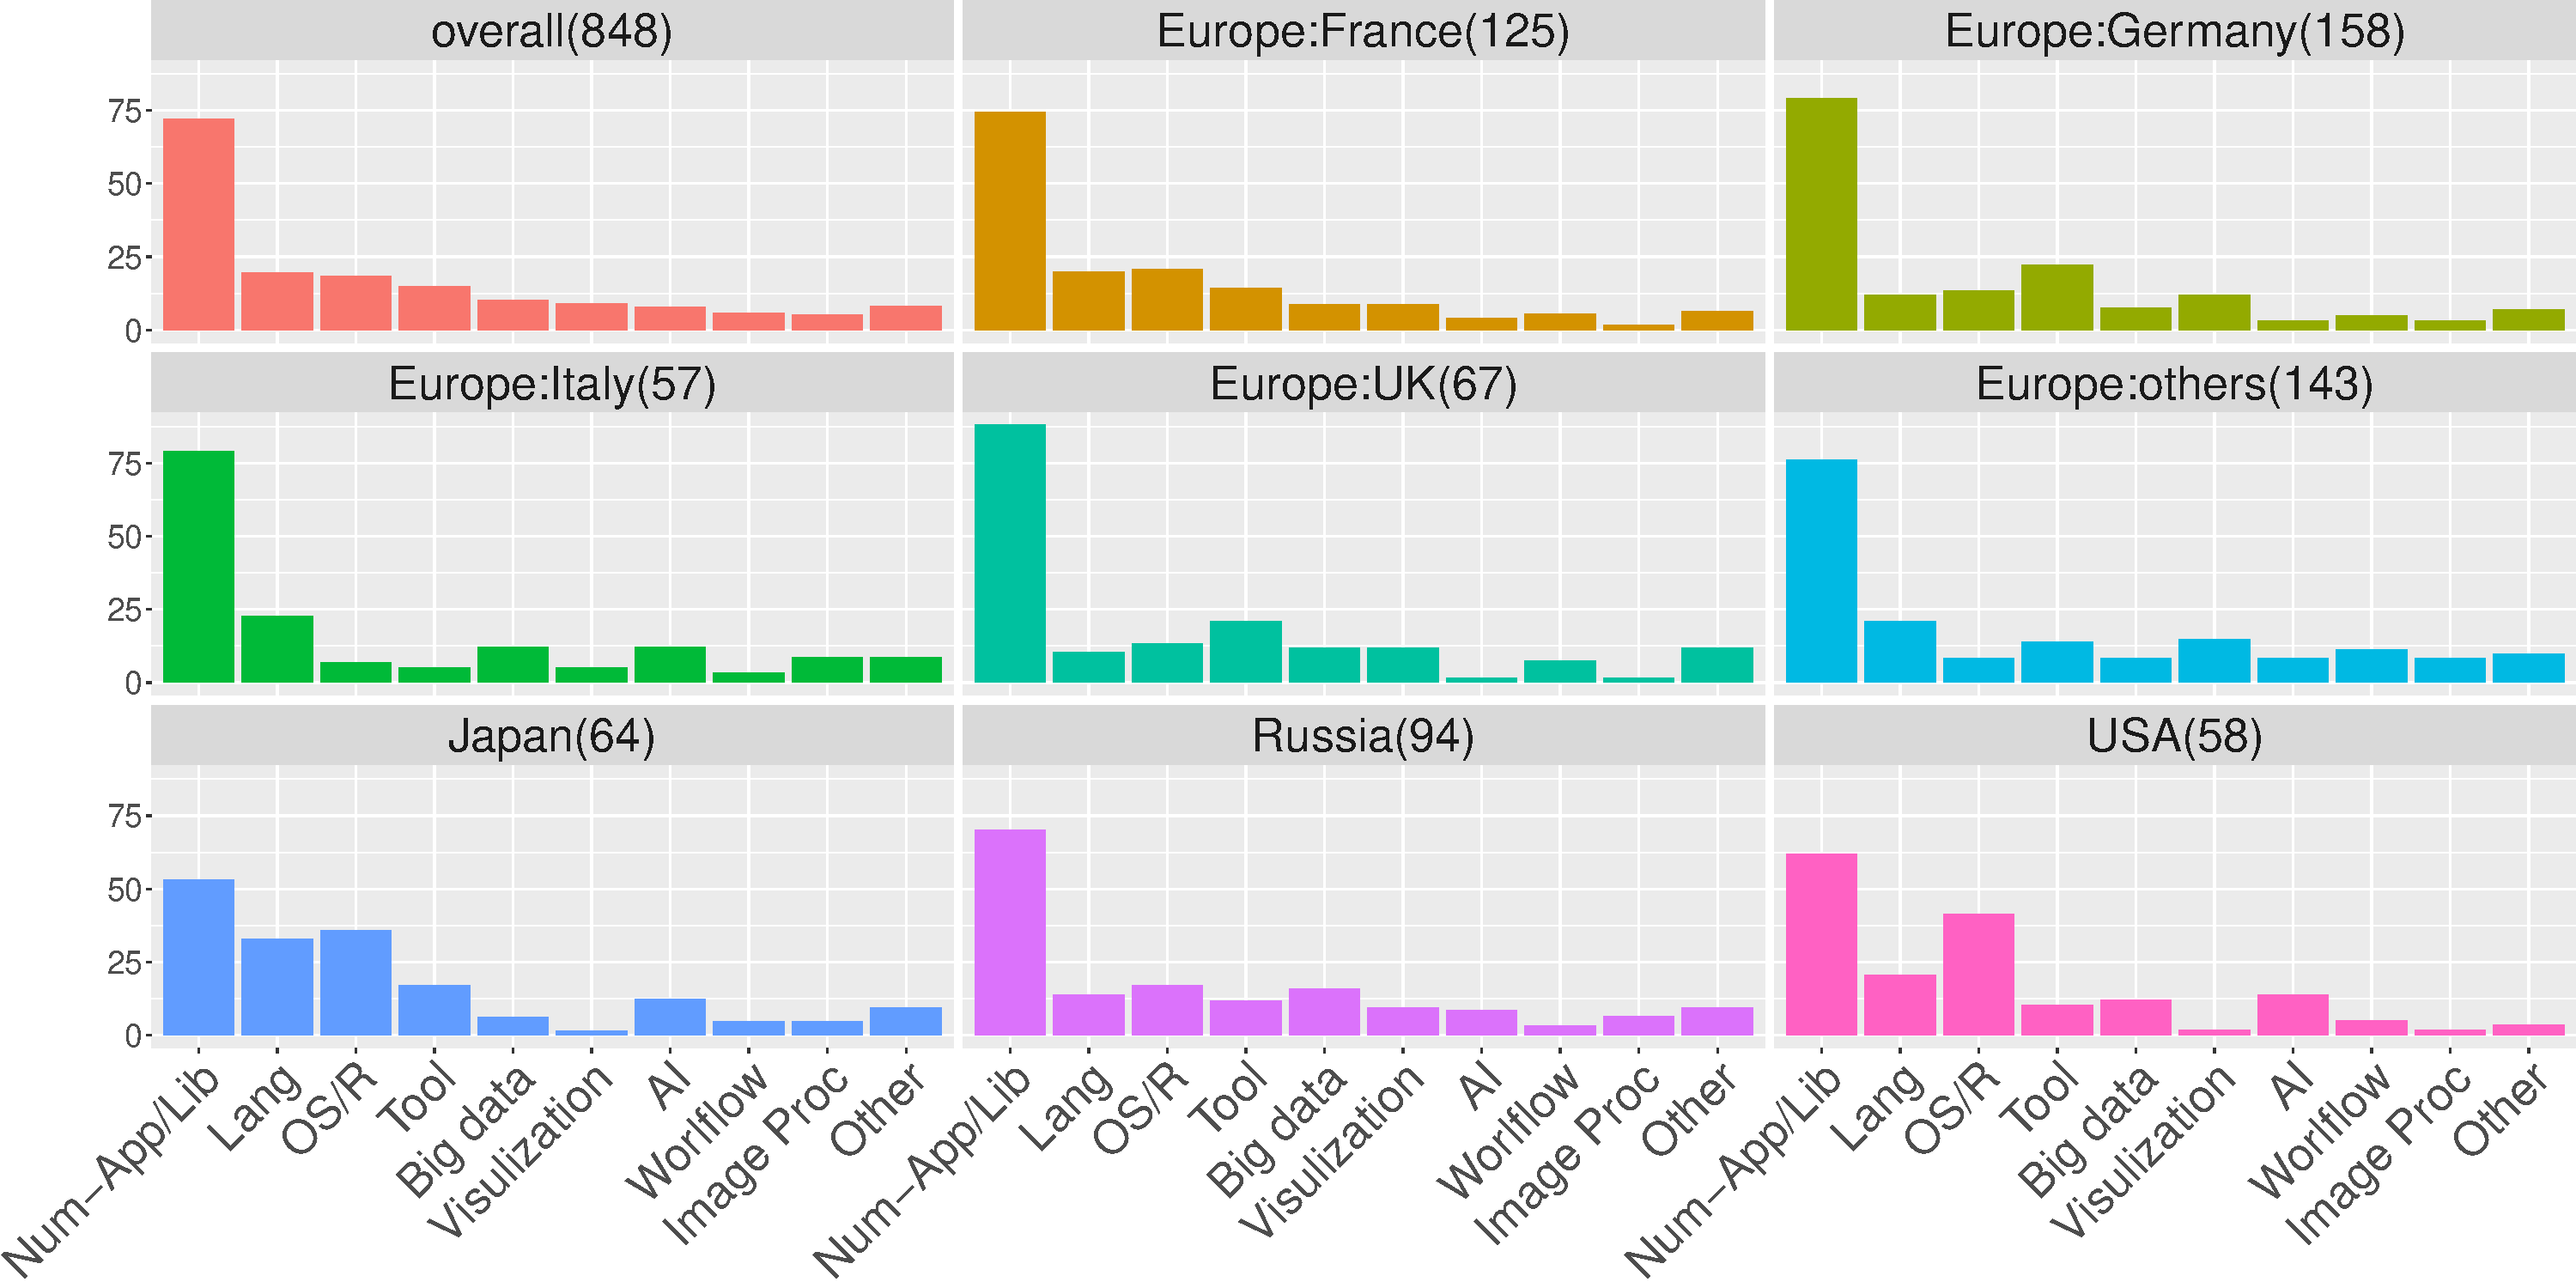
\includegraphics[width=8.7cm]{R-scripts/Q7.pdf}
    \caption{Q7: Working Fields {\it(multiple)}}
    \label{fig:working-fields}
  \end{center}
\end{figure}

\section{Comparison with the ECP survey}\label{sec:ecp}

Although the ECP questionnaire and our questionnaire were designed
independently, there are several questions quite similar. It is also
assumed that some of the participants of our survey
also participated in the ECP survey. However, significant differences
between them can be found. Before going into the details, we clarify
some profiles of the participants in our survey.

\begin{figure}[htb]
  \begin{center}
    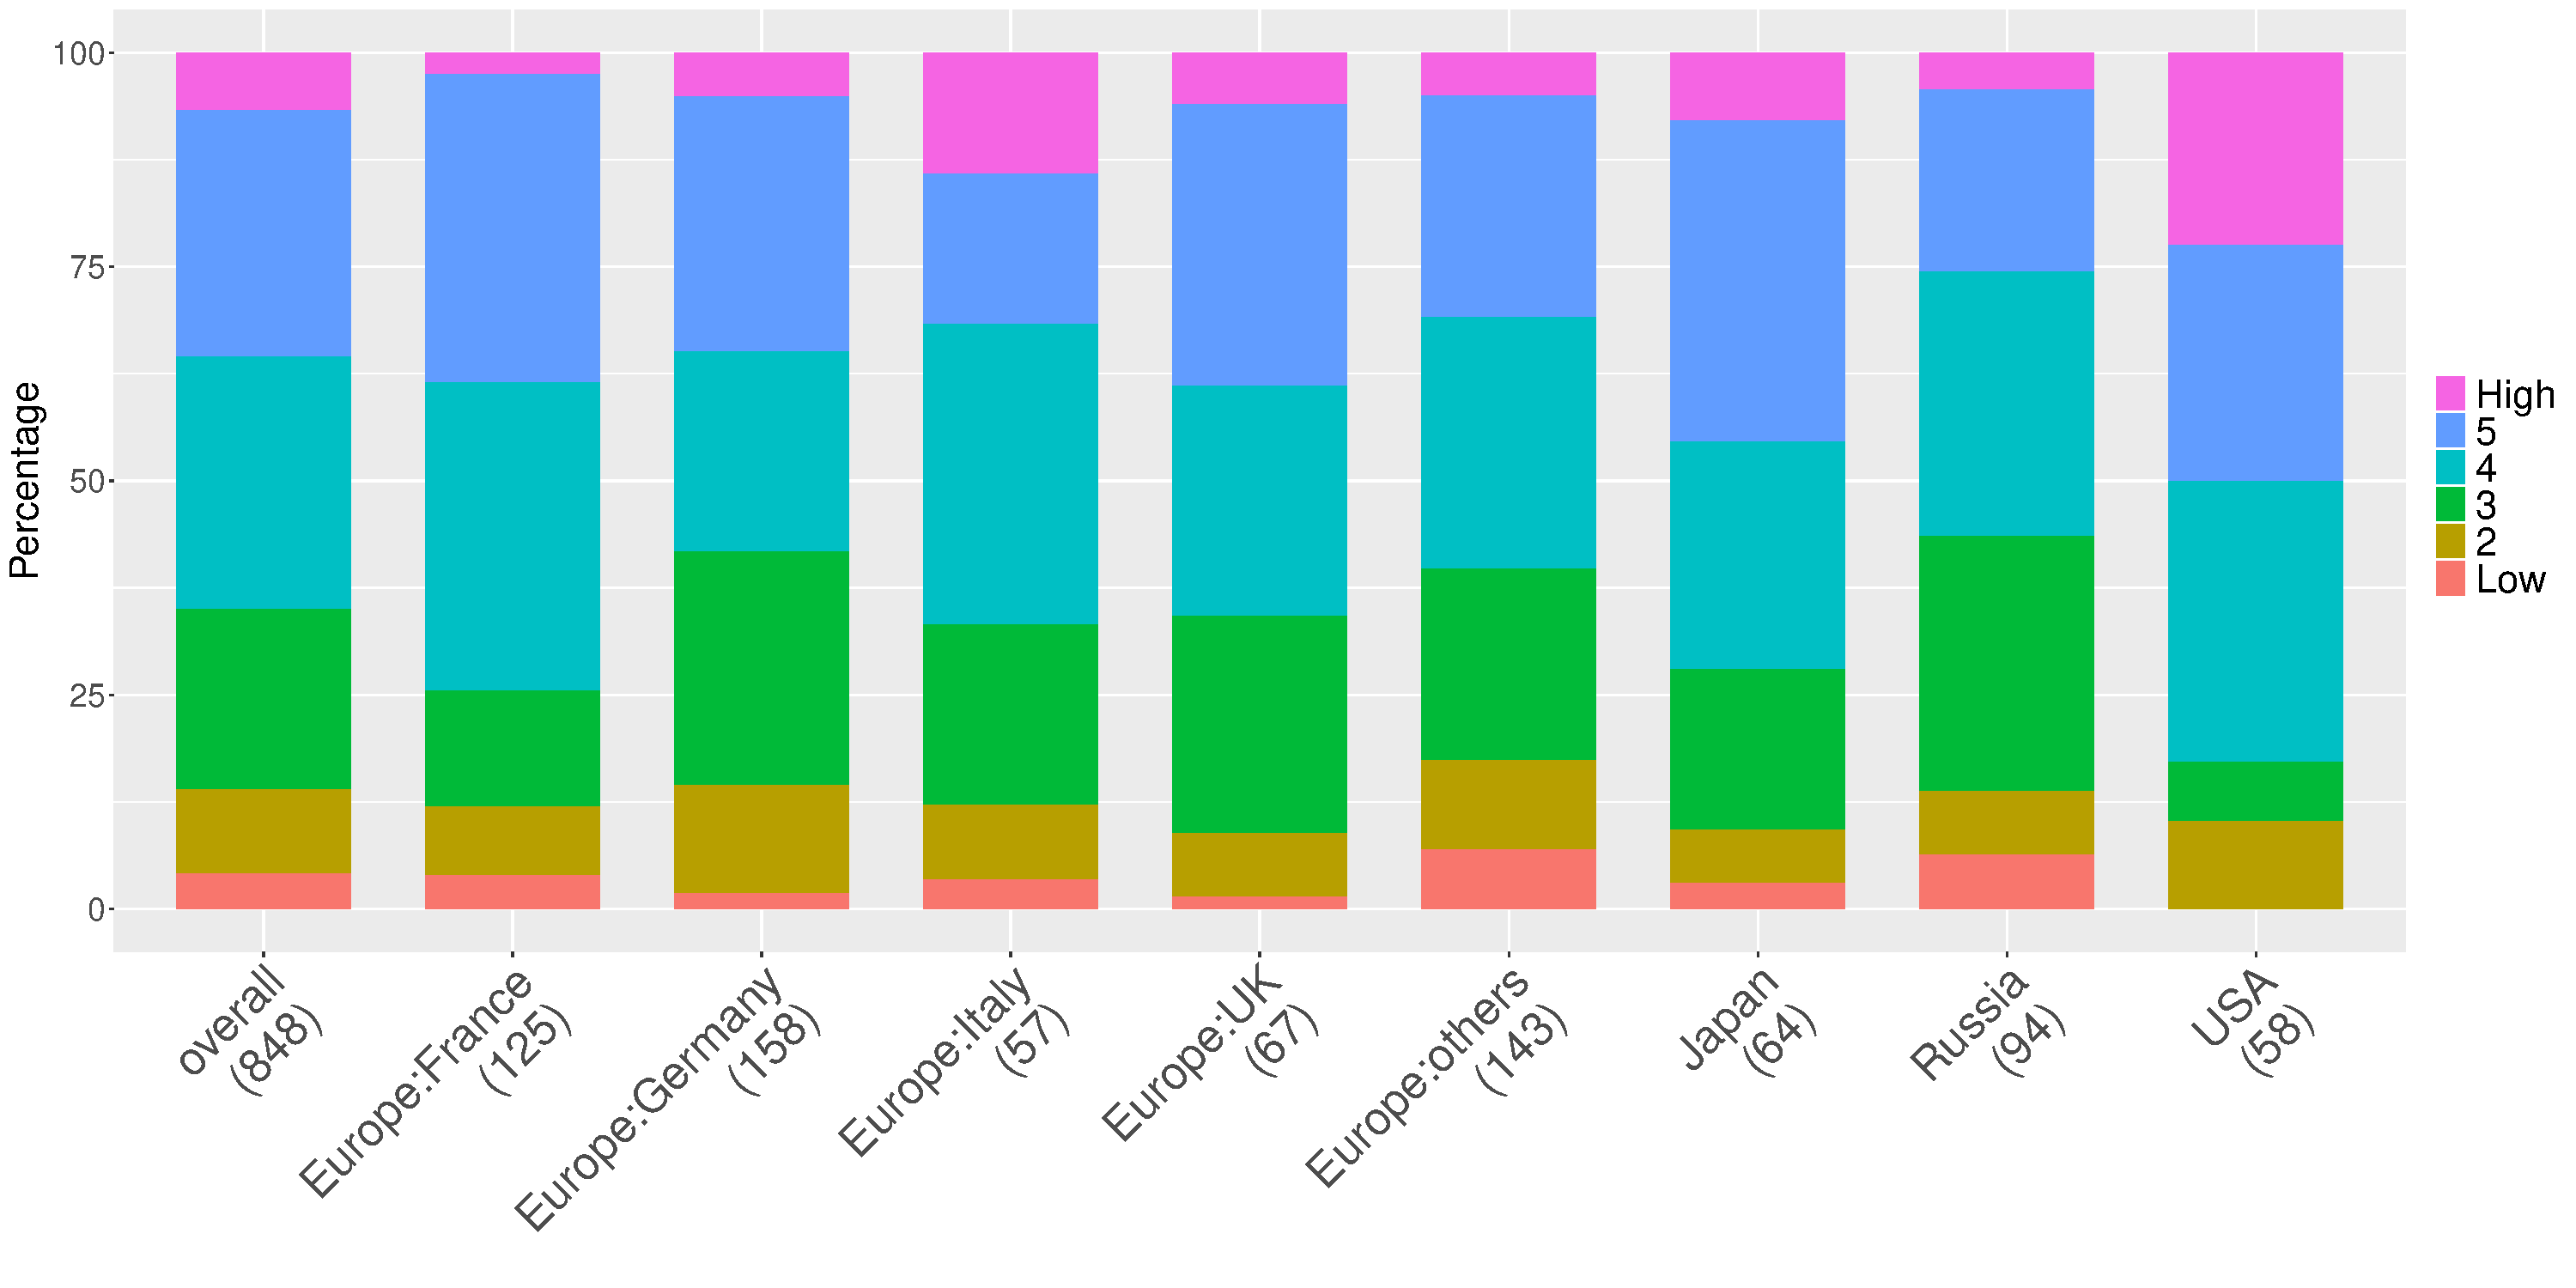
\includegraphics[width=8.7cm]{R-scripts/Q3.pdf}
    \caption{Q3: Self assessment of MPI Skill {\it(single)}}
    \label{fig:mpi-skill}
  \end{center}
\end{figure}

We assumed that the participants in the ECP survey have more
experiences on MPI
programming than the participants of ours. Fig.~\ref{fig:mpi-skill}
shows the results of Q3 asking to rate the participants MPI skill by

themselves in our survey.  In the US case
(right most bar), almost half of participants rate themselves
\myquote{5} or \myquote{High}. This US percentage in having high MPI
skill (\myquote{5} and \myquote{High}) is the highest among
the other countries and nobody in US marked the lowest skill.

\begin{figure}[htb]
  \begin{center}
    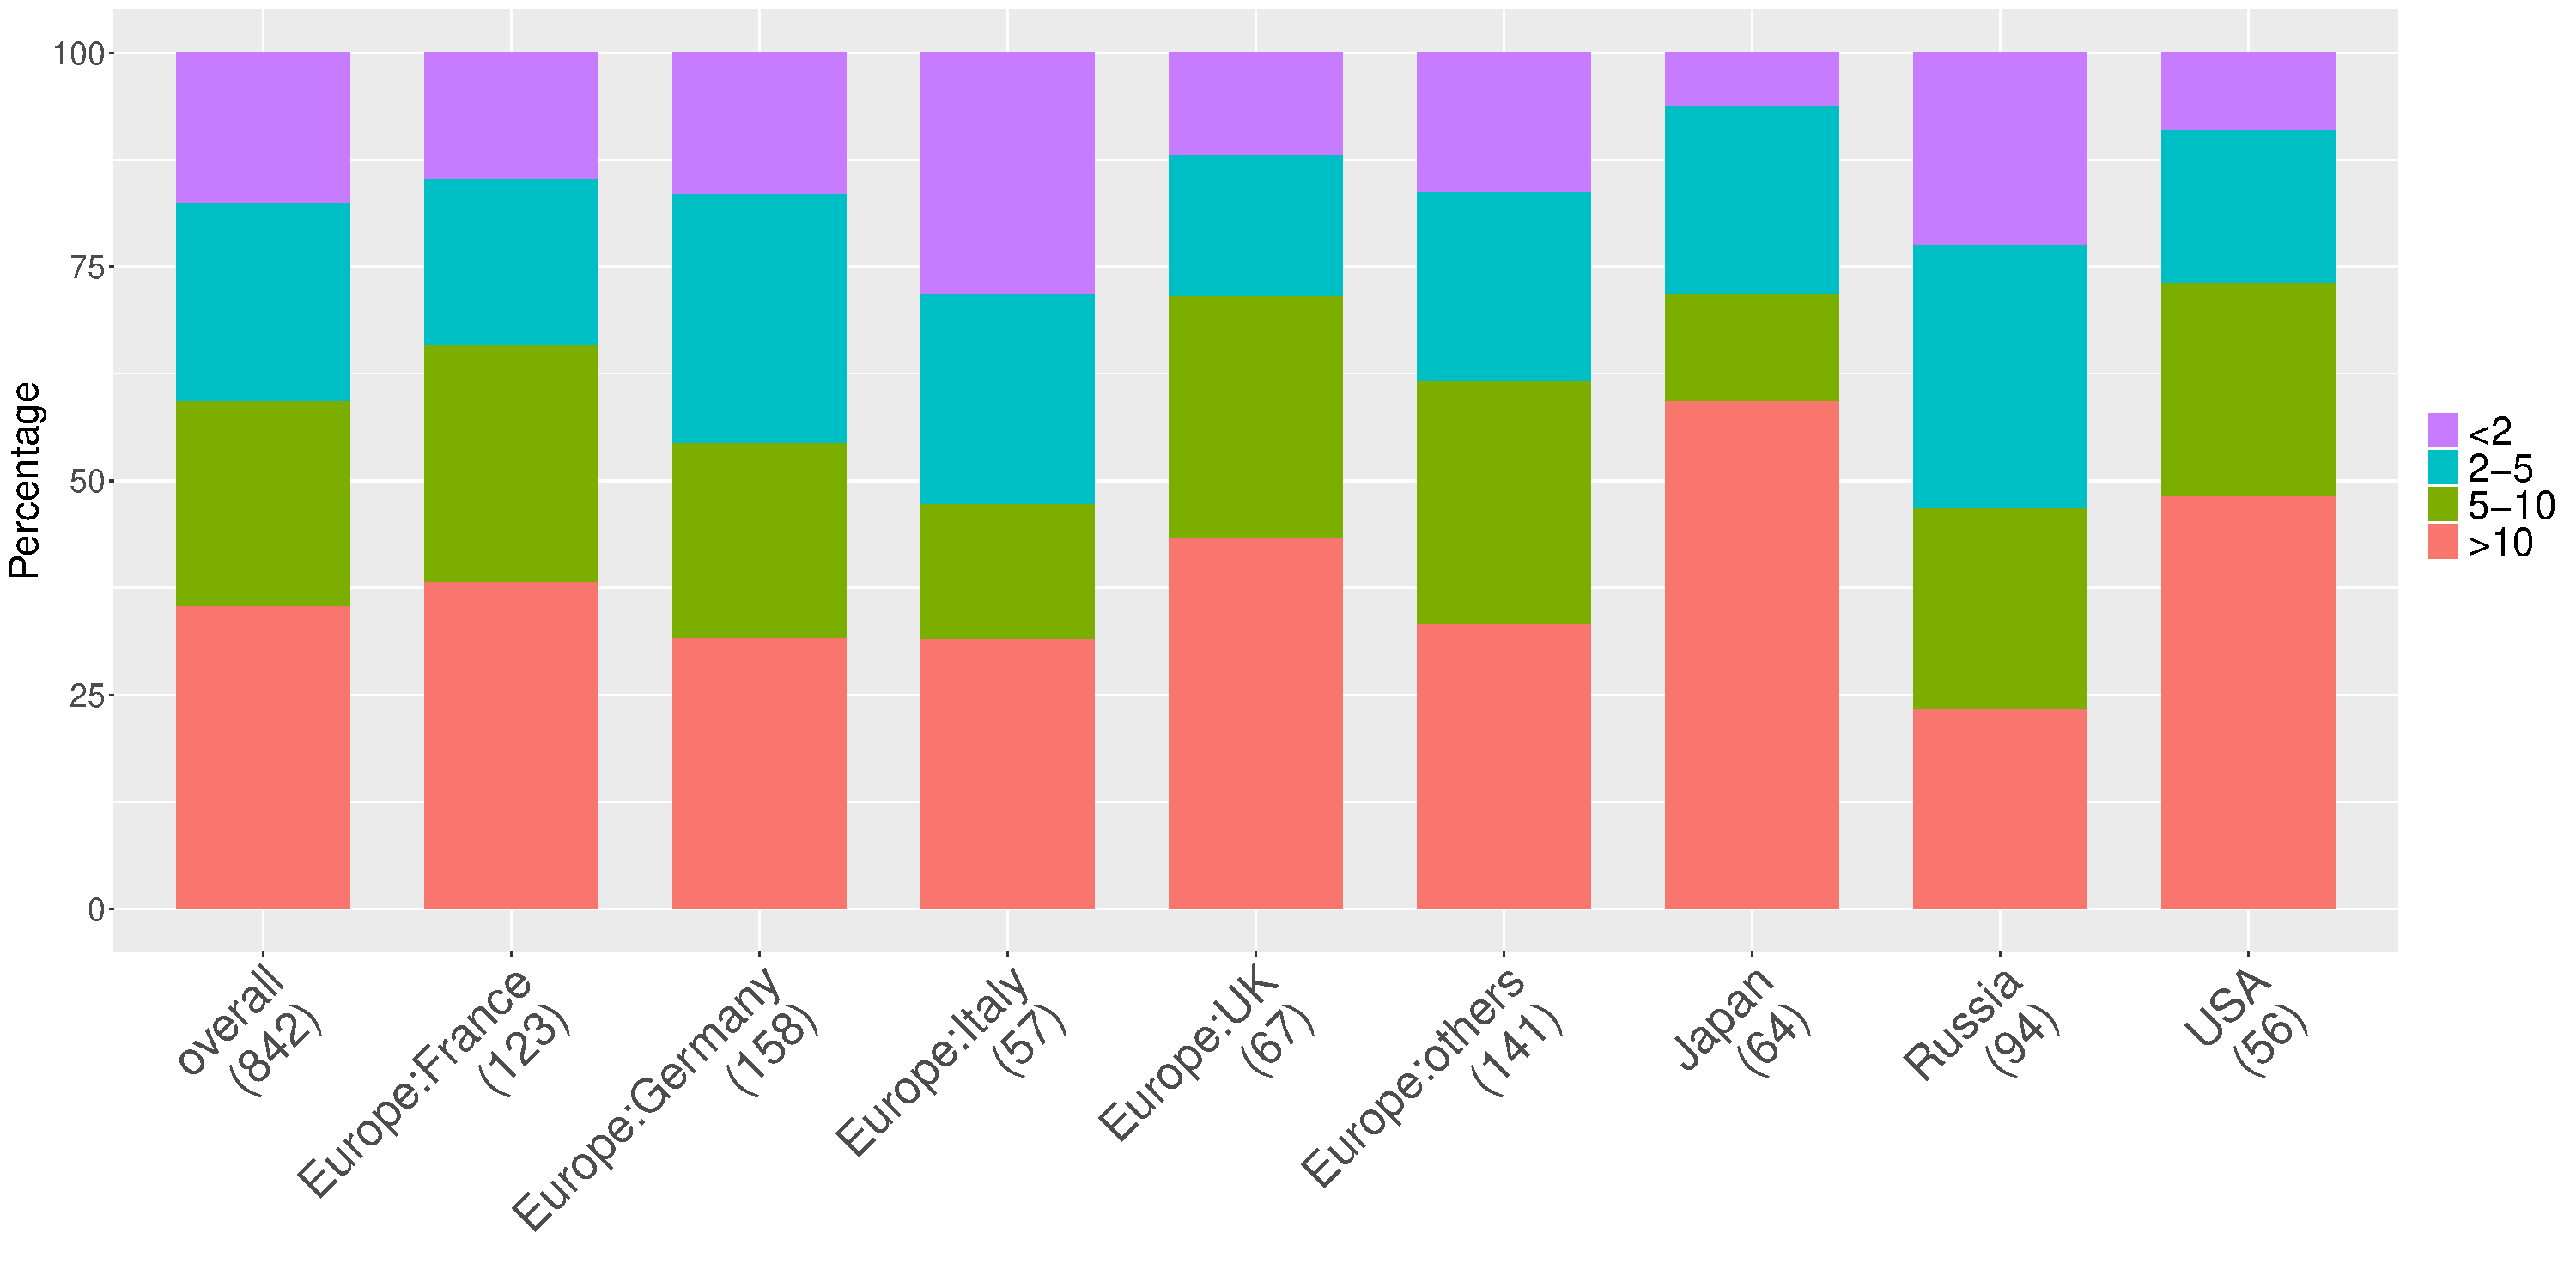
\includegraphics[width=8.7cm]{R-scripts/Q6.pdf}
    \caption{Q6: MPI Experience {\it(single)}}
    \label{fig:mpi-experience}
  \end{center}
\end{figure}

Fig.~\ref{fig:mpi-experience} shows the more interesting result. This
graph is the result of asking {\it How long have you been writing MPI
programs?} and the choices are {\it more than 10 years} (denoted as
\myquote{\textgreater 10}), \myquote{between 5 and 10 years}
(denoted as \myquote{5-10}), \myquote{between 2 and 5 years}
(denoted as \myquote{2-5}) and \myquote{less than 2 years}
(denoted as \myquote{\textless 2}).
Interestingly 9\% of US participants have less than 2 years MPI
experience, but they do no rank their MPI expertise the lowest (Fig.~\ref
{fig:mpi-skill}). Japan followed by USA has the highest percentage in
more than 10 years and has the lowest percentage in less than 2 years
experience. Russia followed by Italy has the highest percentage in
less than 5 years experience (including the less than 2 years
experience case).

We chose three questions from both of out survey and ECP survey that
are very similar and thus the results are comparable
(Table~\ref{tab:comparable-questions}). We will discuss those results
in the following subsections.

\begin{table}[htb]%
  \begin{center}%
    \caption{Comparable Questions}%
    \label{tab:comparable-questions}%
    \begin{tabular}[t]{c|c}
      \hline
      Our Survey & ECP Survey \\
      \hline
      \hline
      \multicolumn{2}{c}{Layering MPI calls (subsection~\ref{sec:mpi-calls})} \\
      \hline
      \begin{minipage}[t]{0.45\hsize}
        Q21: In most of your programs, do you pack MPI function calls into
        their own file or files to have your own abstraction layer for
        communication?  {\it(single)}
      \end{minipage}
      &
      \begin{minipage}[t]{0.45\hsize}
        Q22: Do you have an abstraction layer that hides the MPI calls? Or do
        most of your developers write MPI calls directly? {\it(single)}
      \end{minipage}
      \\
      \hline
      \hline
      \multicolumn{2}{c}{Using MPI Aspects (subsection~\ref{sec:mpi-aspects})} \\
      \hline
      \begin{minipage}[t]{0.45\hsize}
        Q17: What aspects of the MPI standard do you use in your program in its
        current form? {\it(multiple)}
      \end{minipage}
      &
      \begin{minipage}[t]{0.45\hsize}
        Q35: What aspects of the MPI standard do you use in your application in
        its current form? {\it(multiple)}
      \end{minipage}
      \\
      \hline
      \hline
      \multicolumn{2}{c}{Multi-threading (subsection~\ref{sec:mutil-threading})} \\
      \hline
      \begin{minipage}[t]{0.45\hsize}
        Q18: Which MPI thread support are you using? {\it(multiple)}
      \end{minipage}
      &
      \begin{minipage}[t]{0.45\hsize}
        Q59: Which MPI threading option are you using? {\it(single)}
      \end{minipage}
      \\
      \hline
    \end{tabular}%
  \end{center}%
\end{table}%

\subsection{Layering MPI calls}\label{sec:mpi-calls}

\begin{figure}[htb]
  \begin{center}
    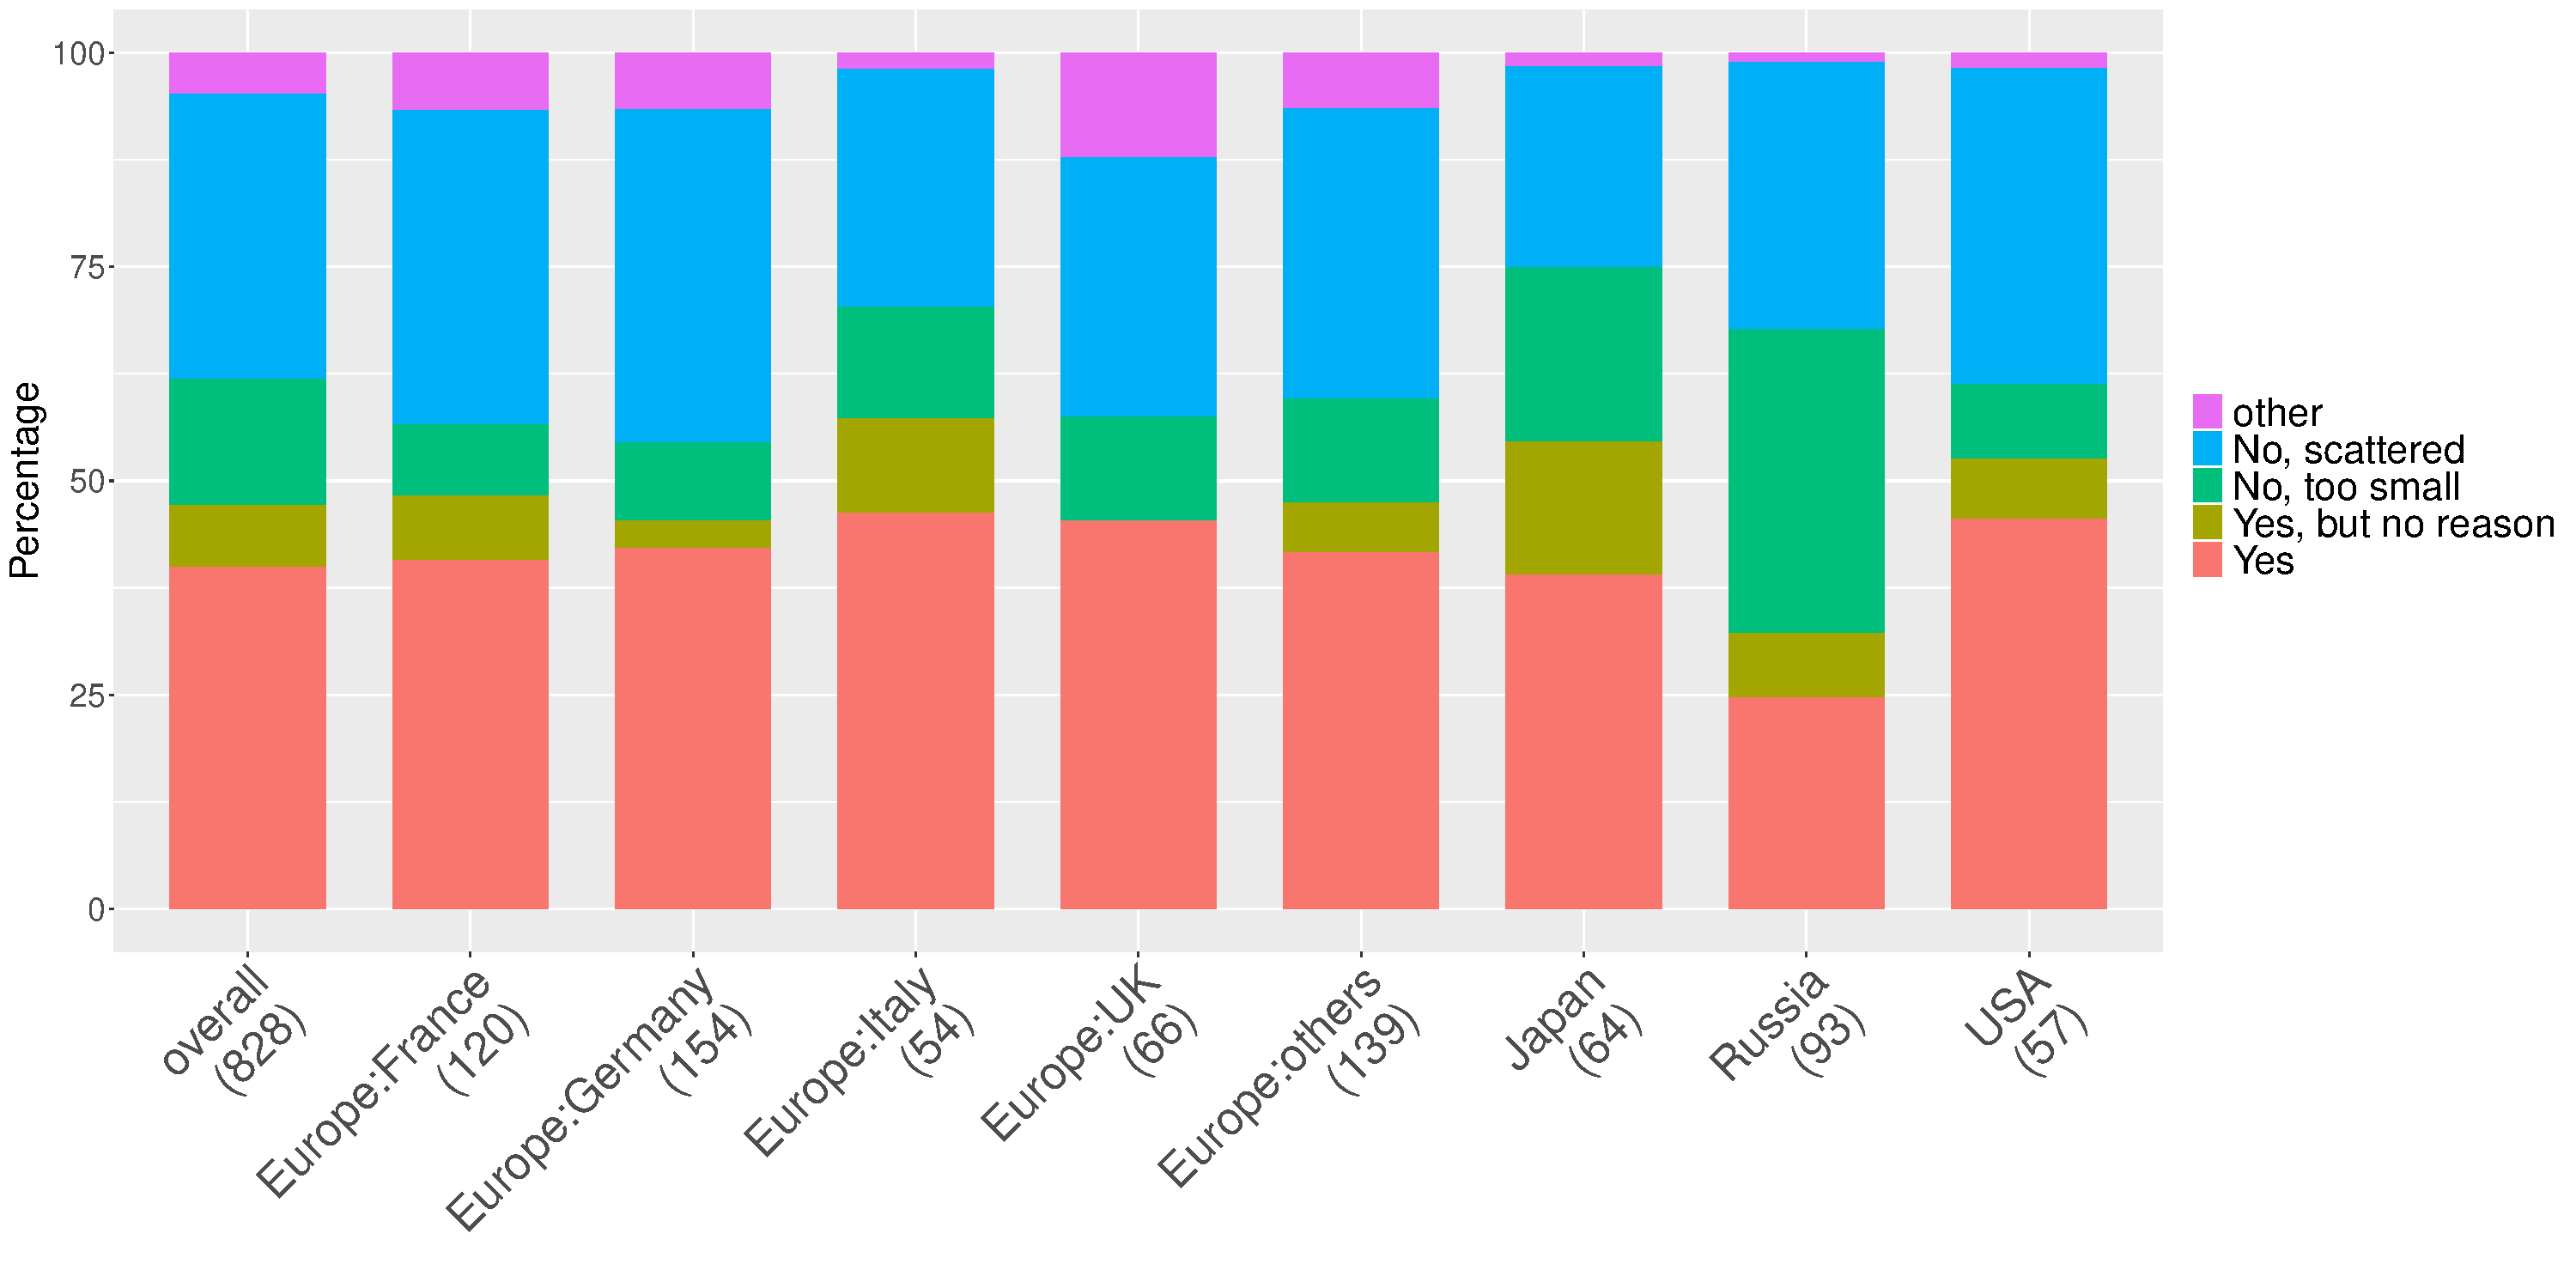
\includegraphics[width=8.7cm]{R-scripts/Q21.pdf}
    \caption{Q21: Layering MPI calls {\it(single)}}
    \label{fig:layering-mpi-calls}
  \end{center}
\end{figure}

Fig.~\ref{fig:layering-mpi-calls} shows the result of our survey and
Table~\ref{tab:layering-mpi-calls} shows the comparison between ours
and the ECP survey. In the ECP survey, the participants are categorized
into two groups; application development (AD) and system technology
(ST). It is interesting that the percentage of the participants having
MPI layer(s) in our survey is roughly 50\% even in the US, whilst the
ratio of yes and no is approximately $6:4$ in the ECP survey.
Having a closer look at Fig.~\ref{fig:layering-mpi-calls}, the answer,
\myquote{No, my program is too small to do that}, dominates in Russia. In
the other countries, the participants having a packing layer occupies
40-50\%.

\begin{table}[htb]%
  \begin{center}%
    \caption{Layering MPI calls}\label{tab:layering-mpi-calls}%
    \begin{tabular}{c|c||c|c||c|c|c}%
      \hline%
      \multicolumn{2}{c||}{Choice} & \multicolumn{2}{c||}{Our Survey [\%]} &
      \multicolumn{3}{c}{ECP [\%]} \\
      \cline{3-7}%
      \multicolumn{2}{c||}{} & overall & USA & AD & ST & AD+ST \\
      \hline%
      \hline%
      Yes & - & 40 & 46 & & & \\
      & no reason & 7 & 7 & & & \\
      \cline{2-4}%
      & (sum) & 47 & 53 &  79 & 46 & 62 \\
      \hline%
      \hline%
      No & too small & 15 & 9 & & & \\
      & - & 33 & 37 & & & \\
      \cline{2-4}%
      & (sum) & 48 & 46 & 21 & 54 & 38 \\
      \hline%
      \hline%
      Other & - & 5 & 2 & - & - & - \\
      \hline%
    \end{tabular}%
  \end{center}%
\end{table}%

\subsection{Using MPI Aspects}\label{sec:mpi-aspects}

The Q35 in the ECP survey and Q17 in our survey are almost equivalent
questions, although choices are somewhat
different. Fig.~\ref{fig:using-mpi-aspects} shows the result of our
survey and Table~\ref{tab:using-mpi-aspects} shows the comparison
between ECP's and ours on the same choices. As shown in
Fig.\ref{fig:using-mpi-aspects}, the
using aspects can be categorixed in three groups; A) more frequently
used (point-to-point and collectives), B) second frequently used
(\myquote{Datatypes}, \myquote{with OpenMP}, \myquote{Communicator}, and \myquote{One-sided}), and C) less
frequently used (\myquote{PMPI}, \myquote{Persistent}, and
\myquote{dyn. process} (dynamic process).
It should be noted that all these less frequently used features were
already introduced and standardized in MPI 2.2 which was release in
2009. Despite the 10-year appearance, those features failed to get
popular.

\begin{figure}[htb]
  \begin{center}
    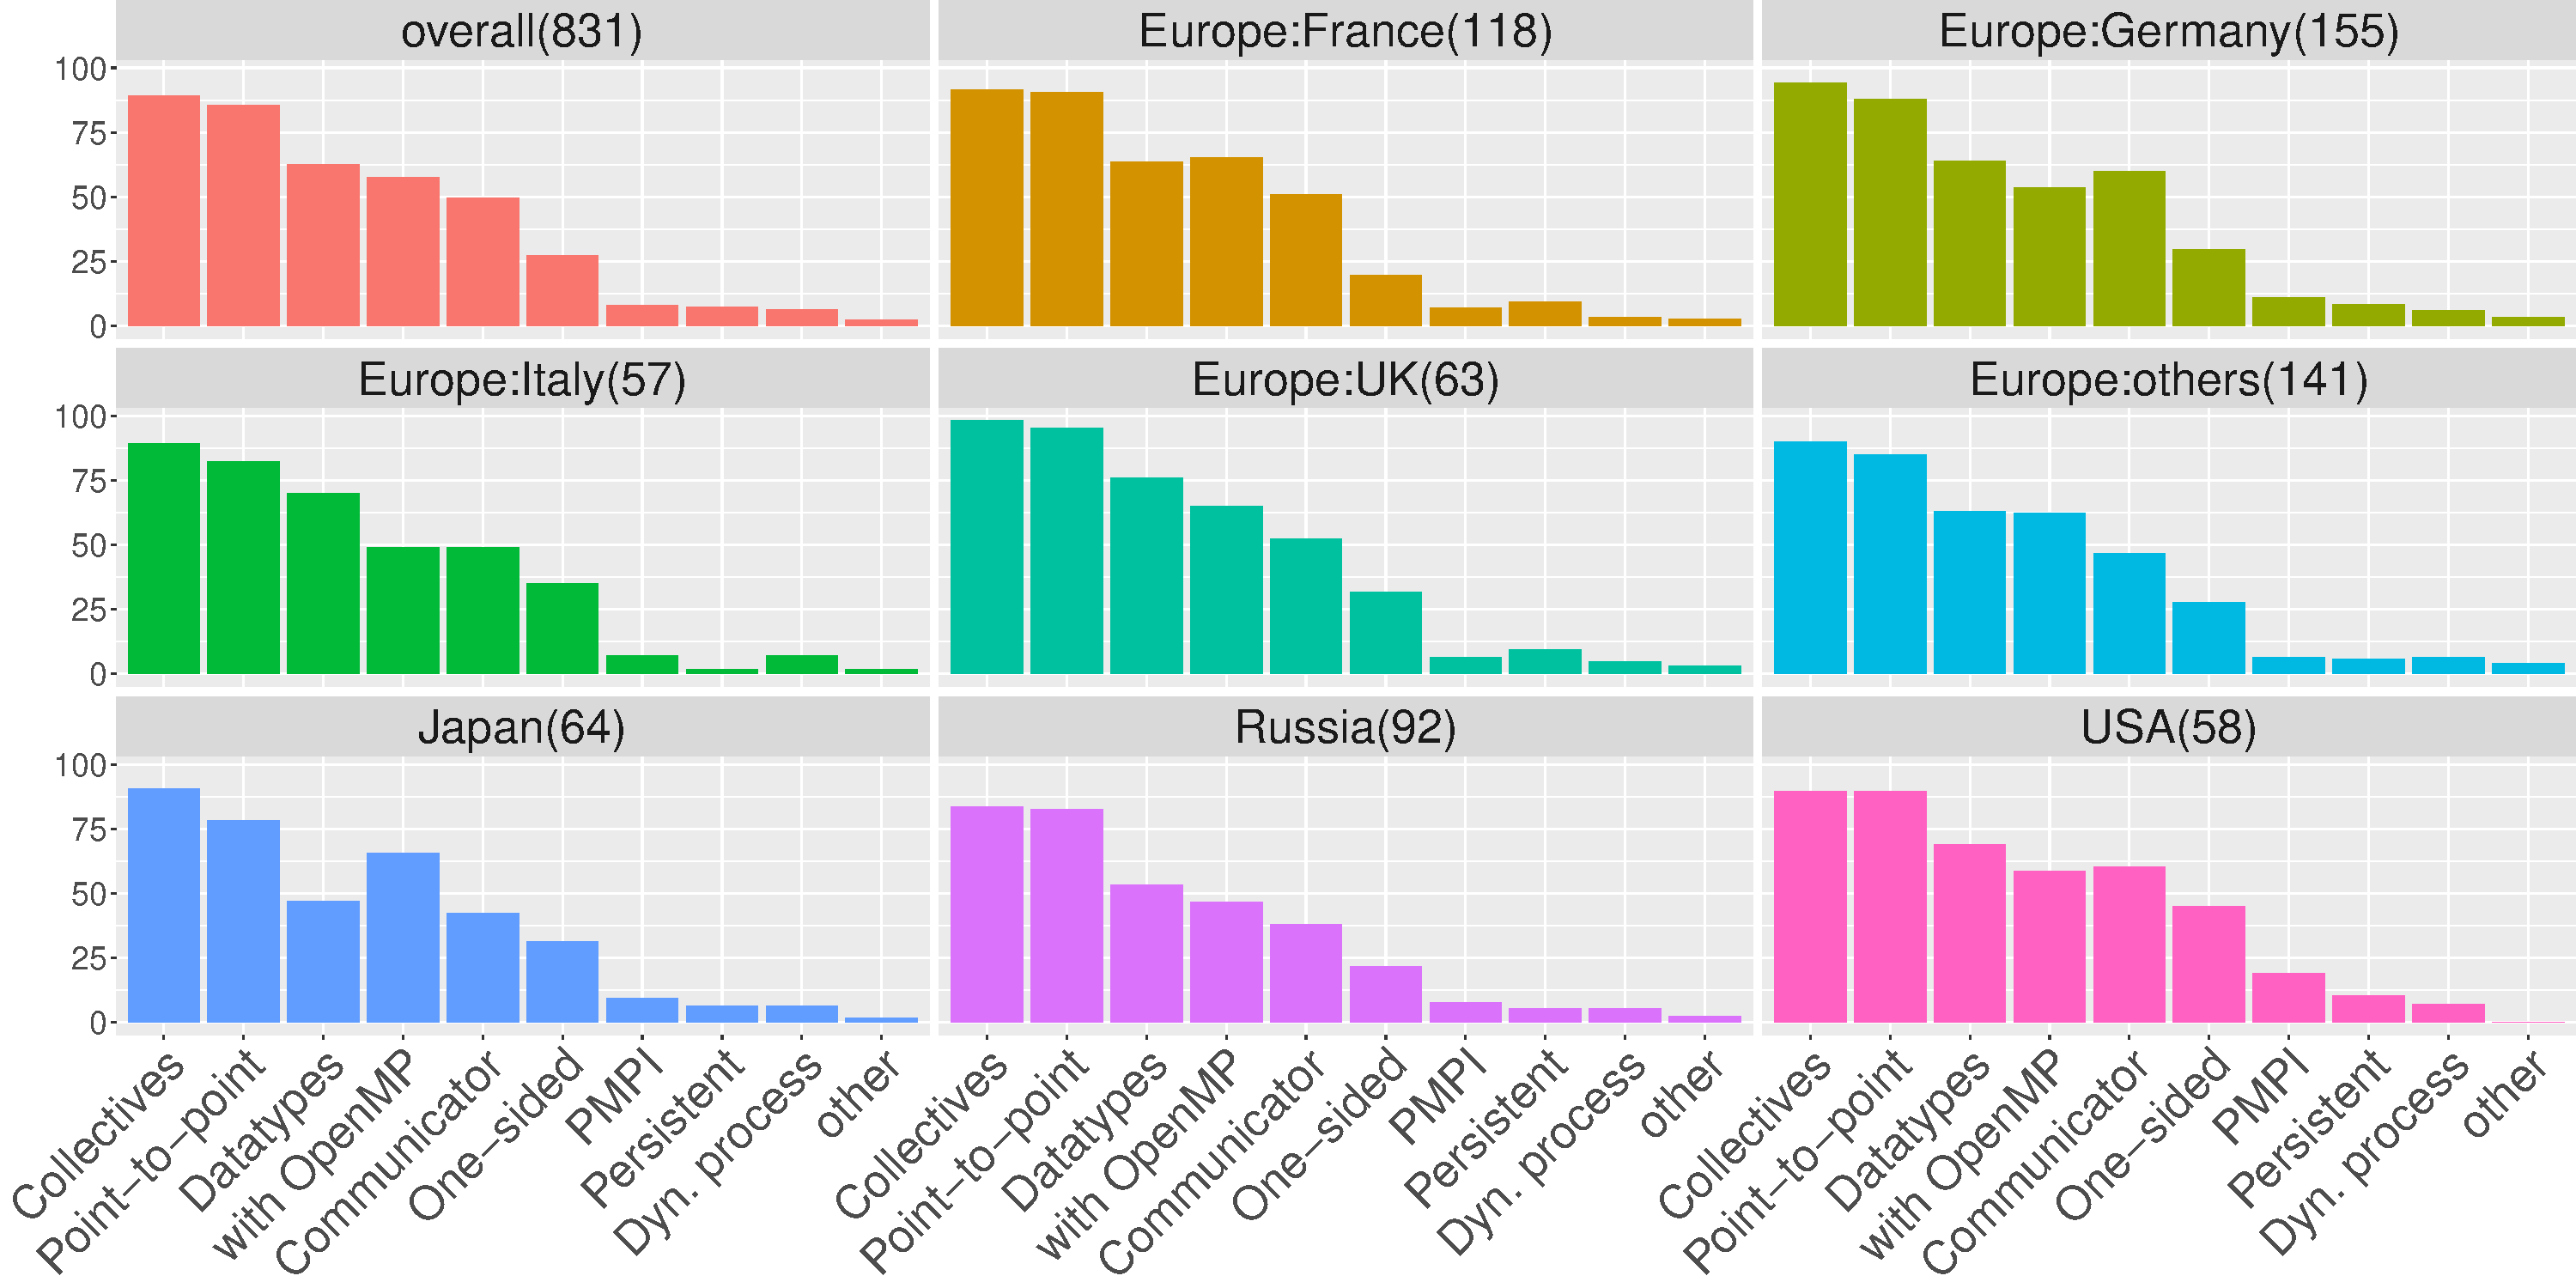
\includegraphics[width=8.7cm]{R-scripts/Q17.pdf}
    \caption{Q17: Using MPI Aspects {\it(multiple)}}
    \label{fig:using-mpi-aspects}
  \end{center}
\end{figure}

Most notable difference between our survey and the ECP survey is the
datatype (Table~\ref{tab:using-mpi-aspects}). The percentage in
datatype in ECP is 23\% and the percentage in our survey is more
than 60\% in both overall and USA. In the ECP survey, there are three
questions asking using MPI aspects in different usage scenarios;
\begin{enumerate*}
\item current,
\item exascale, and
\item performance critical
\end{enumerate*}.%
In all three questions, the percentages of using datatype are low.

\begin{table}[htb]%
  \begin{center}%
    \caption{Using MPI Aspects}\label{tab:using-mpi-aspects}%
    \begin{tabular}{c||c|c||c|c|c}%
      \hline%
      Choice & \multicolumn{2}{c||}{Ours [\%]} &
      \multicolumn{3}{c}{ECP {\scriptsize (current usage)} [\%]} \\
      \cline{2-6}%
      & overall & USA & AD & ST & {\small AD+ST} \\
      \hline%
      Collectives & 89 & 90 & 86 & 75 & 80 \\
      Point-to-point & 85 & 90 & 96 & 79 & 88 \\
      Datatype & 63 & 69 & 25 & 21 & 23 \\
      Communicator & 50 & 60 & 68 & 54 & 61 \\
      {\small One-sided (RMA)} & 27 & 45 & 36 & 7 & 21 \\
      PMPI & 8 & 19 & 11 & 0 & 14 \\
      \hline%
      \multicolumn{6}{r}{\small * Both are multiple answer questions} \\
      \multicolumn{6}{r}{\small ** Common choices in both surveys are shown}\\
    \end{tabular}%
  \end{center}%
\end{table}%

Fig.~\ref{fig:skill-and-aspects} is the addition. This graph is a
heatmap of the cross-tab analysis between Q3 asking MPI skill and Q16
asking unknown MPI features. The darker the color of a cell, the
higher the frequency (Legend combined with color bar can be found at
the bottom of the figure. The numbers in the legend cells are
percentages). Less frequent rows (1 is the lowest skill and 6 is the
highest skill) in this figure are
omitted to increase readability. Natural thinking may conclude
that the higher the MPI skill, lesser the unknown MPI features. The
result is quite interesting, the less used features in
Fig.~\ref{fig:using-mpi-aspects}, PMPI, persistent, and dynamic
process, are almost independent from the MPI skill.

\begin{figure}[htb]
  \begin{center}
    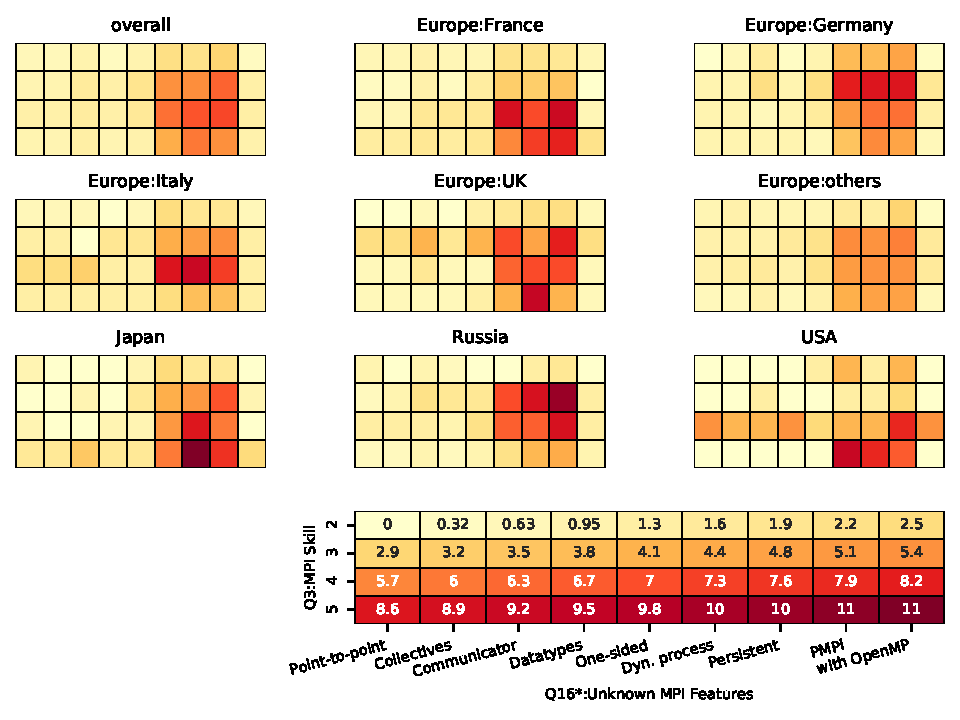
\includegraphics[width=8.7cm]{Figs/Q3-Q16.pdf}
    \caption{Q3-Q16: MPI Skill {\it(single)} and Unknown MPI Features {\it(multiple)}}
    \label{fig:skill-and-aspects}
  \end{center}
\end{figure}

The similar situation can be seen in the cross-tab analysis between Q6
and Q16 (Fig.~\ref{fig:experience-and-aspects}). It would be plausible,
the longer the MPI experience, the less unknown features. However,
some countries (France, UK and Japan) in these heatmaps show that the
longer the experience, the higher the percentage of having unknown
features. This may indicate that the long experienced MPI users may
not catch up the newly introduced MPI features.

\begin{figure}[htb]
  \begin{center}
    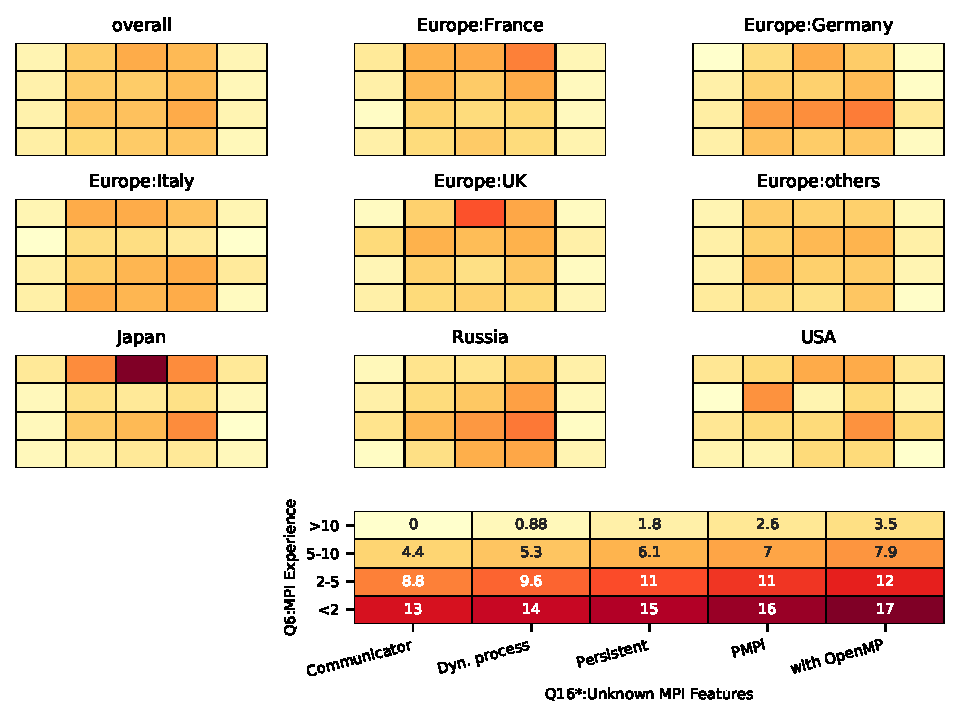
\includegraphics[width=8.7cm]{Figs/Q6-Q16.pdf}
    \caption{Q6-Q16: MPI Experience {\it(single)} and Unknown MPI Features {\it(multiple)}}
    \label{fig:experience-and-aspects}
  \end{center}
\end{figure}

This may indicate
that the MPI standard is very profound. Even the most basic
send/receive functions, although they look very simple and natural,
they require deep knowledge such as possibility of deadlock, timing of
buffer access, blocking and non-blocking, and so on.

Fig.~\ref{fig:useless-features} is the result of Q27 asking \myquote{What MPI
feature(s) are NOT useful for your application?}. Although many
participants think MPI has no {\it not useful features}, fairly amount of
participants think the dynamic process feature not useful. Thinking
of the fact that the dynamic process feature is not used by the most
participants (Q17, Fig.~\ref{fig:using-mpi-aspects}), this result is
quite interesting.
This tendency is also reported in \cite{10.1145/3295500.3356176}.

\begin{figure}[htb]
  \begin{center}
    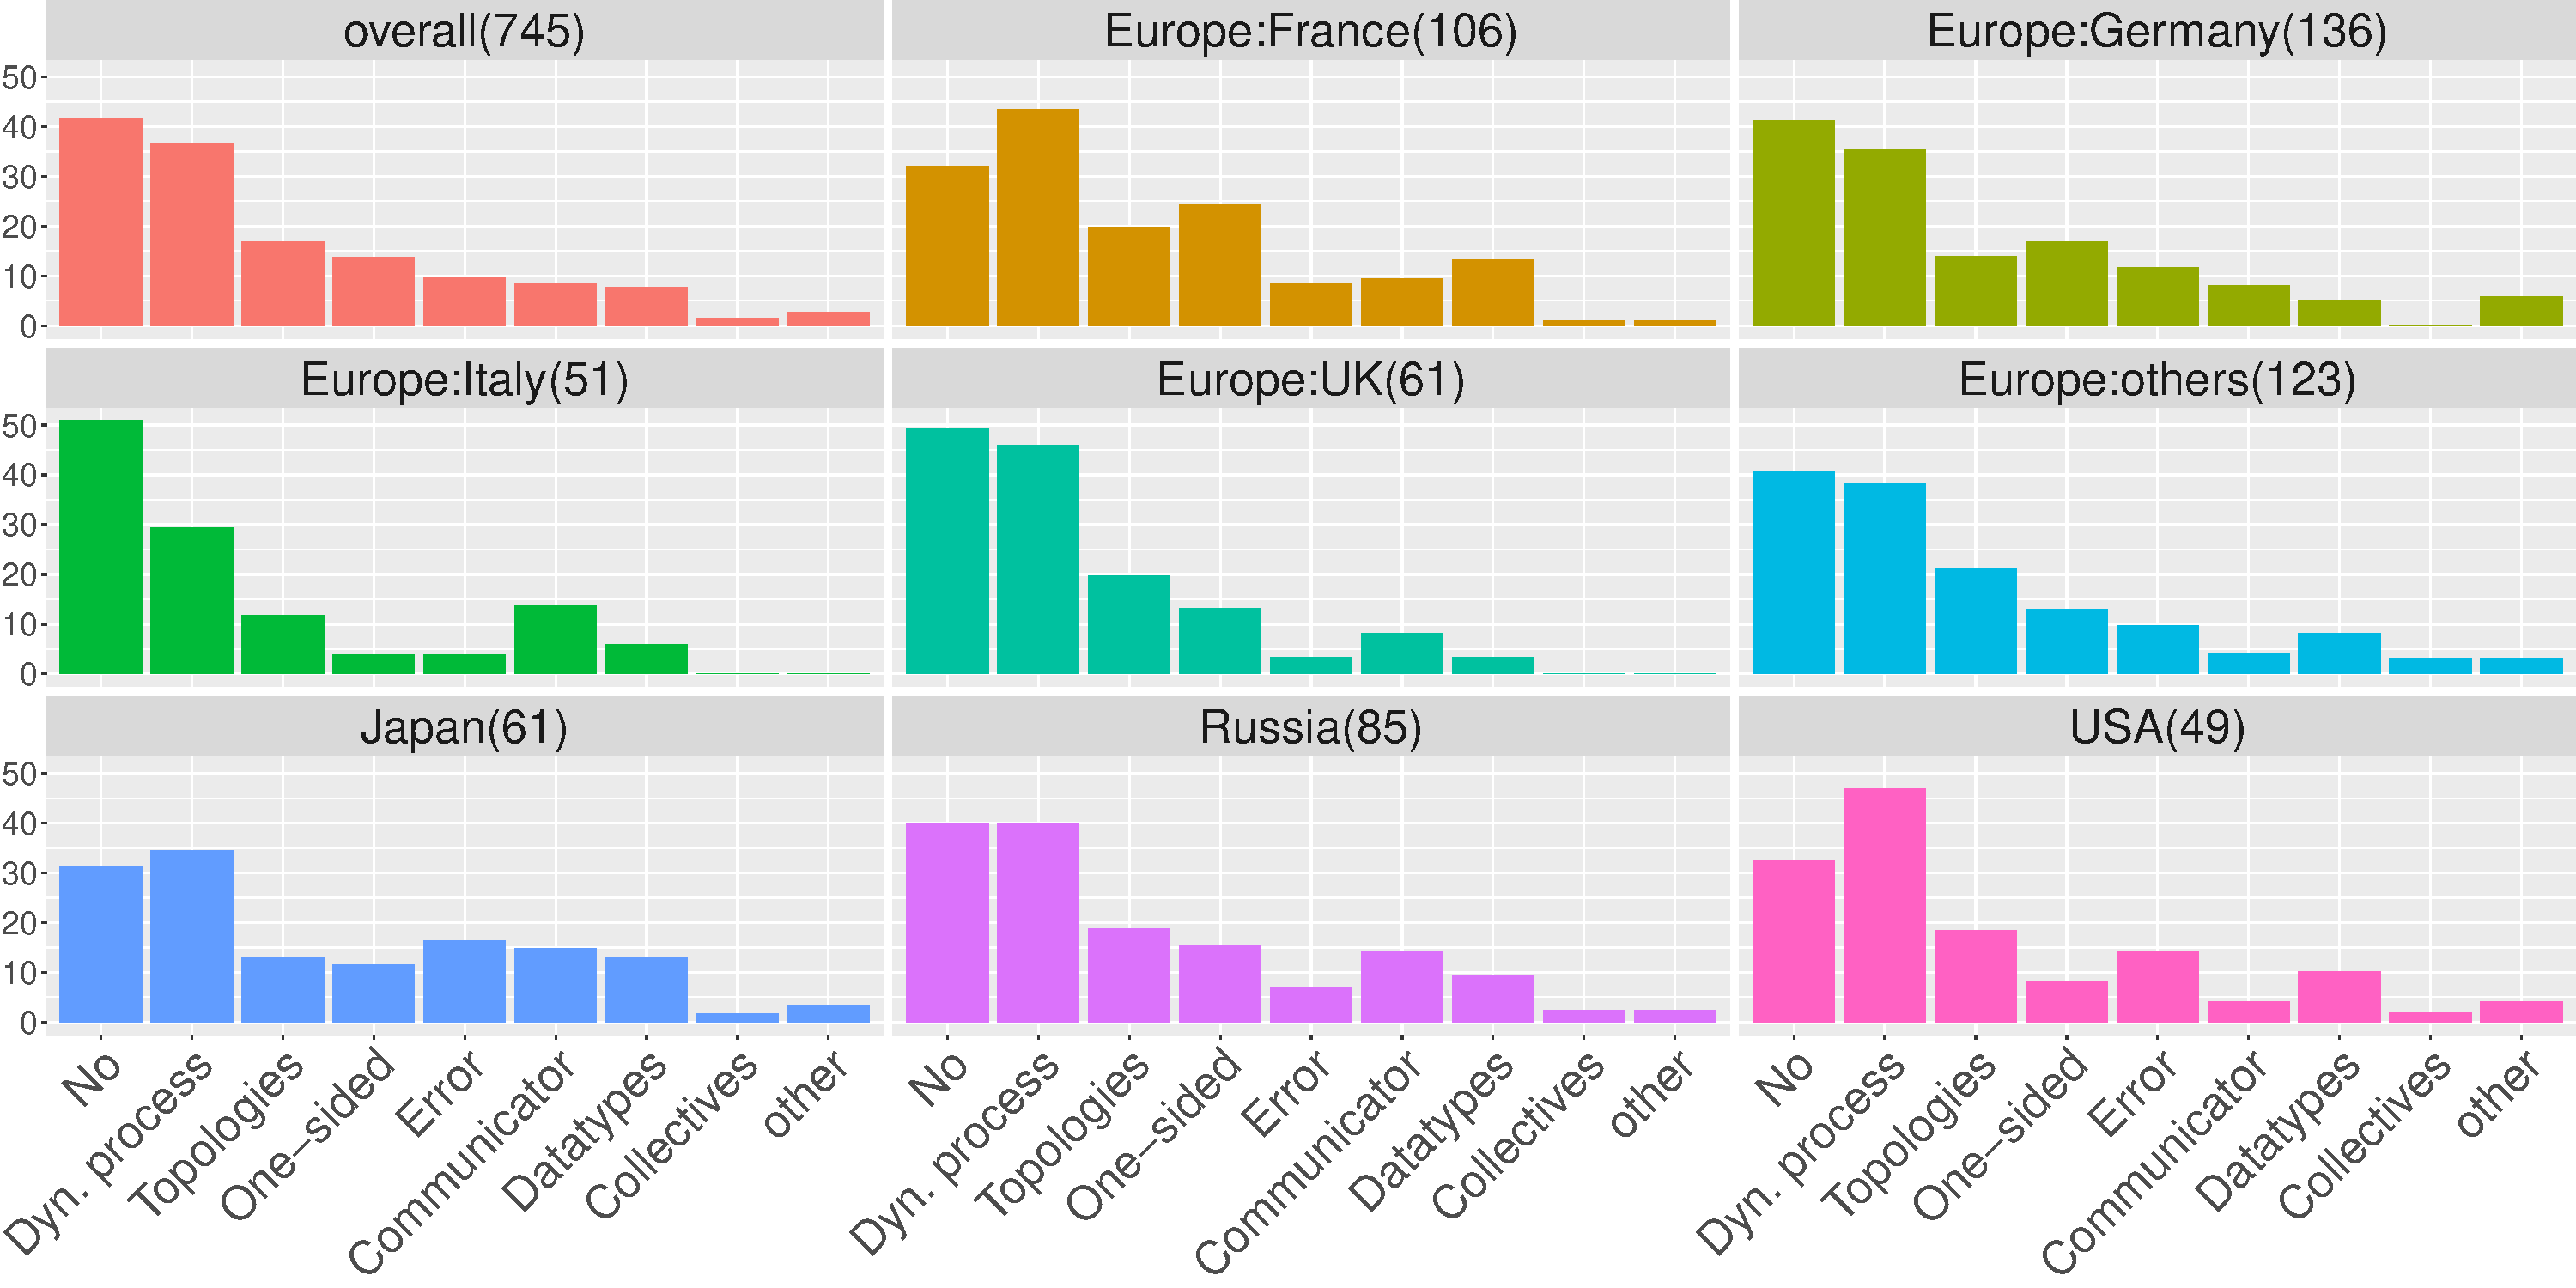
\includegraphics[width=8.7cm]{R-scripts/Q27.pdf}
    \caption{Q27: Useless Features {\it(multiple)}}
    \label{fig:useless-features}
  \end{center}
\end{figure}

The dynamic process feature is on the
border of process management and communication, since the process
creation itself is obviously out of the scope of the MPI standard,
while the communication between the existing (MPI) processes and newly
create (MPI) processes must be defined in the standard. Indeed, the
implementation of dynamic process creation spreads many parts of a
computing system: MPI library, process manager, job scheduling system
and system operation. This complexity might make the use of the
dynamic process creation hard and impractical for MPI users and the
un-usefulness of dynamic process may not come from the MPI standard.

\subsection{Multi-threading}\label{sec:mutil-threading}

The difference between our survey and the ECP survey can also be found on
the question asking multi-threading support. Fig.~\ref{fig:multi-thread}
shows the result of our survey and Table~\ref{tab:multi-thread} shows
the difference. Note that our question is multiple-answer and the ECP
question is single-answer. In both surveys (USA and ECP), the
percentage of using {\tt MULTIPLE} is the highest excepting the AD
case. However, the percentage of the choice \myquote{I don't know}
is fairly larger than ours. This may sound contradictory because the
ECP participants would be more experienced MPI users.

\begin{table}[htb]%
  \begin{center}%
    \caption{Multi-threading}\label{tab:multi-thread}%
    \begin{tabular}{c||c|c||c|c|c}%
      \hline%
      Choice & \multicolumn{2}{c||}{Our Survey [\%]} &
      \multicolumn{3}{c}{ECP {\it(single)} [\%]} \\
      \cline{2-6}%
      & overall & USA & AD & ST & AD+ST \\
      \hline%
      SINGLE & 29 & 22 & \multicolumn{3}{c}{\scriptsize (no corresponding choice)} \\
      FUNNELED & 18 & 13 & 18 & 18 & 18 \\
      SERIALIZED & 12 & 10 & 18 & 18 & 18 \\
      MULTIPLE & 22 & 31 & 18 & 32 & 25 \\
      never used & 23 & 16 & \multicolumn{3}{c}{\scriptsize (no corresponding choice)} \\
      not know & 14 & 8 & 25 & 25 & 25\\
      \hline%
    \end{tabular}%
  \end{center}%
\end{table}%

The usage of {\tt MULTIPLE} in US is also the highest among the major
regions (Fig.~\ref{fig:multi-thread}). France and Germany have the
same trend. In Italy, Japan, Russia and the
other European countries, the percentages of \myquote{I don't know}
are the highest. In UK, the percentage of using {\tt SINGLE} is the
highest.

\begin{figure}[htb]
  \begin{center}
    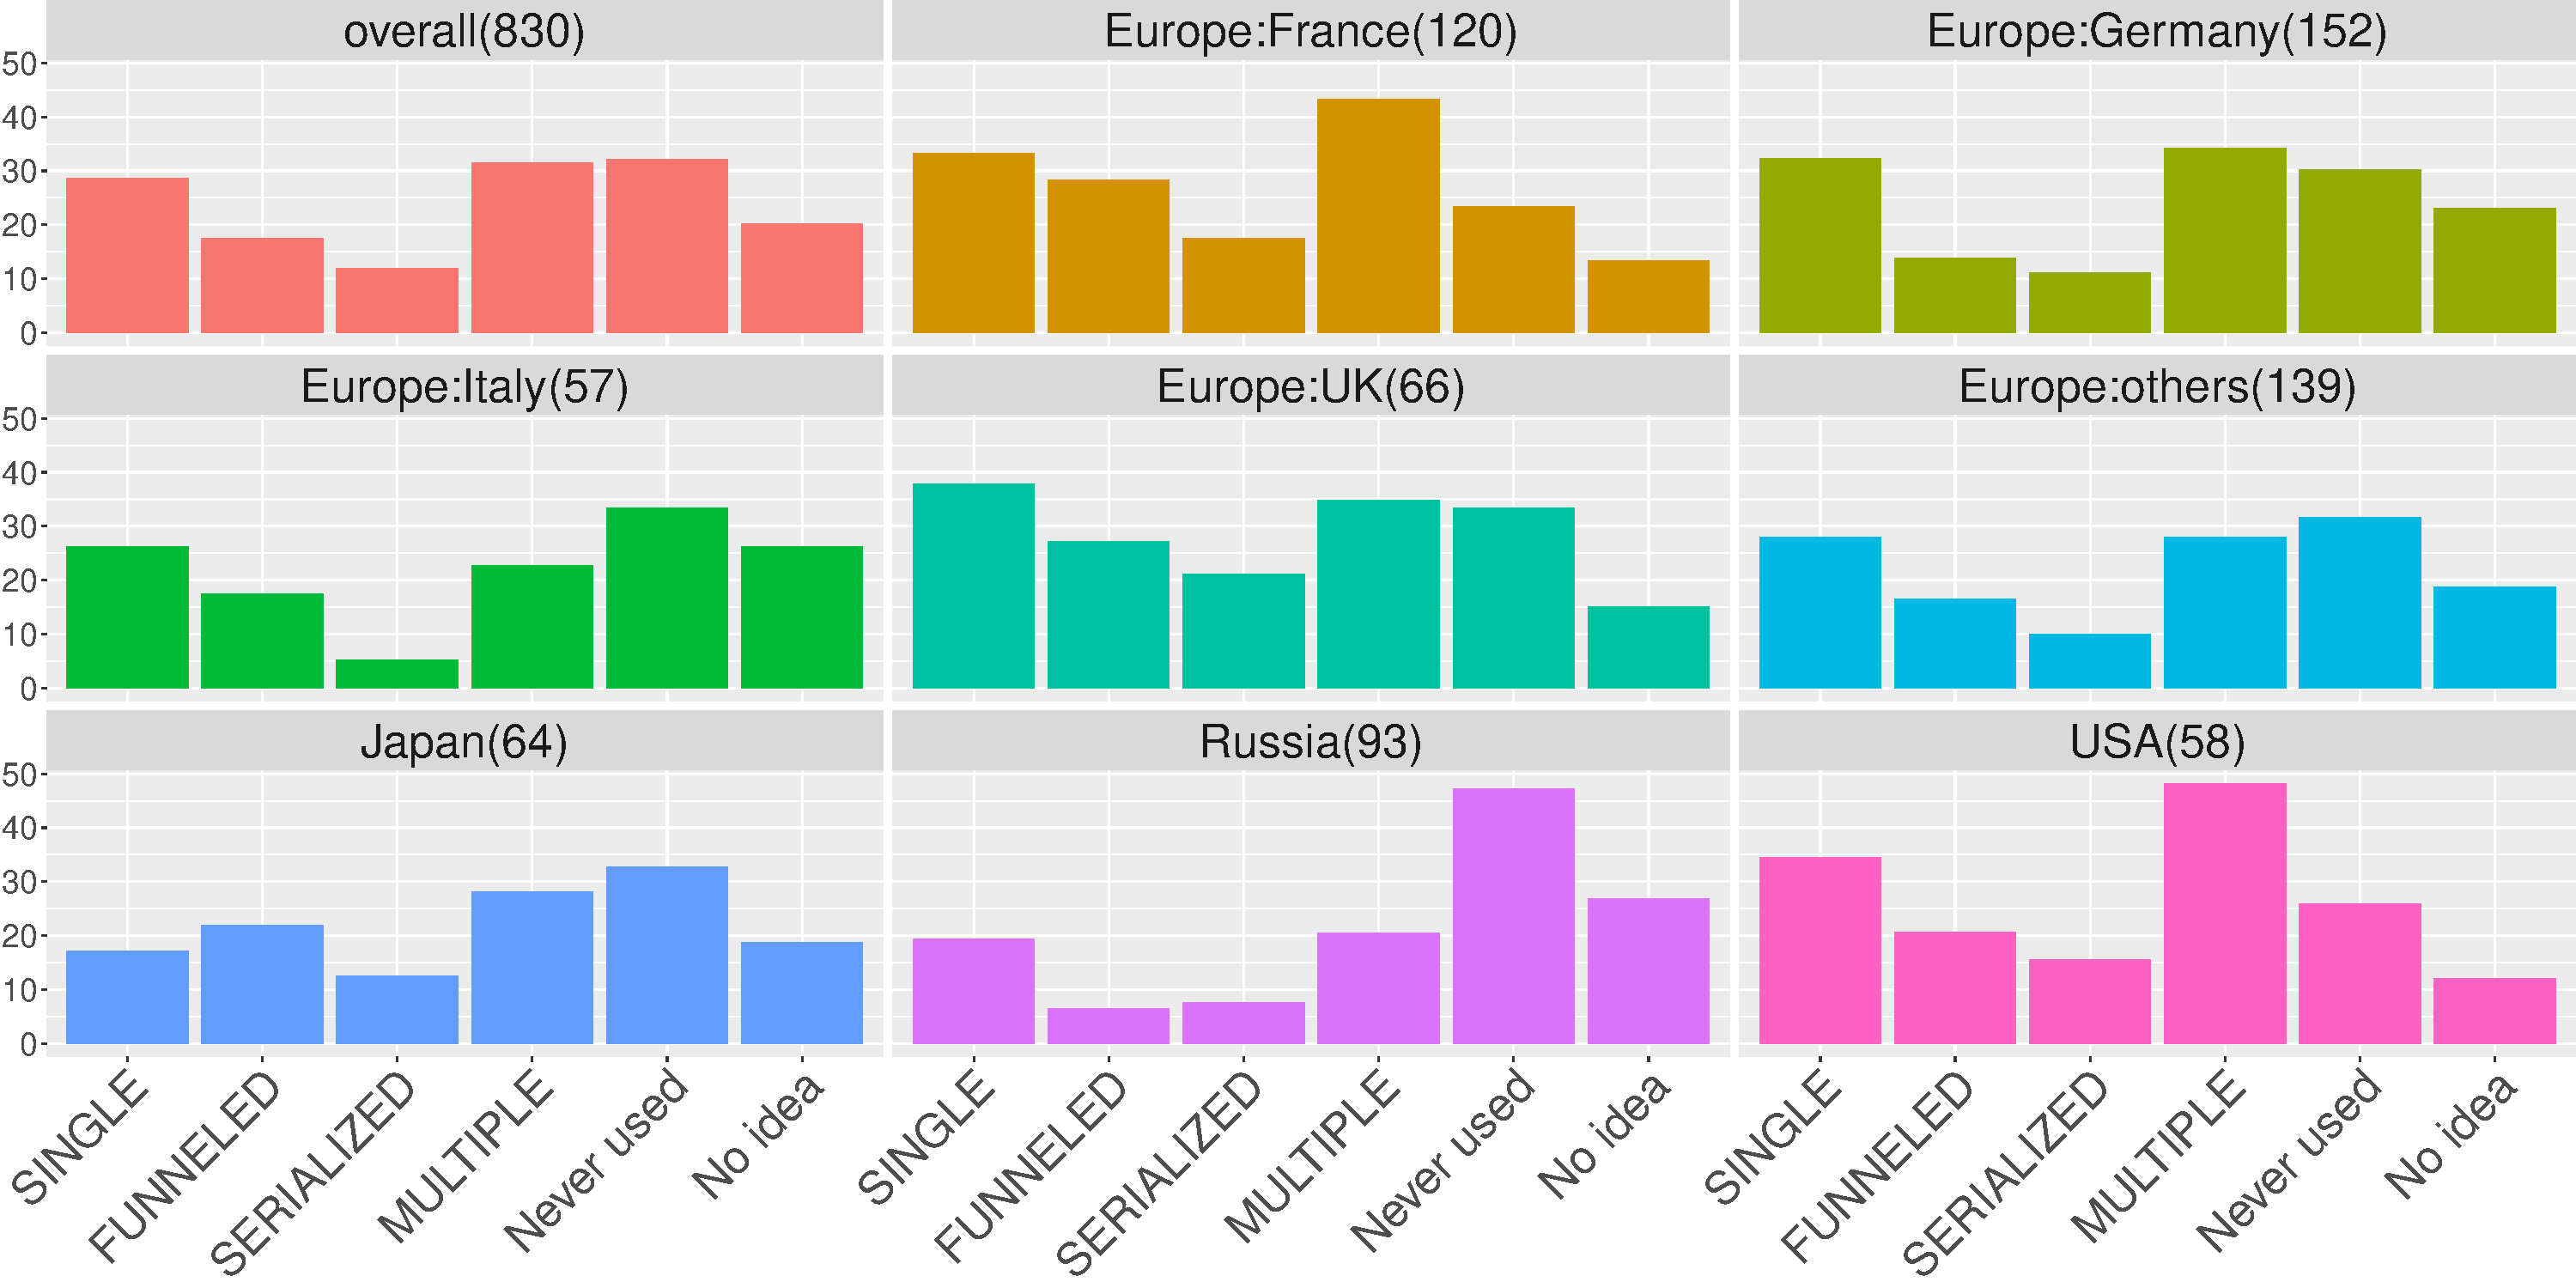
\includegraphics[width=8.7cm]{R-scripts/Q18.pdf}
    \caption{Q18: Multi-threading {\it(multiple)}}
    \label{fig:multi-thread}
  \end{center}
\end{figure}

Remember this is a multiple answer
question. Table~\ref{tab:multi-thread-raw} shows the top 7 of the
percentages of raw answers (combined answers) of the
overall. These top 7 percentages occupy about 85\% in
total. Nearly half
participants answered \myquote{never used} or \myquote{no idea.} The
numbers in parenthesis in this table are the percentage of
participants excluding those who answered \myquote{never used} or
\myquote{no idea}. Half of threading-aware participants are using {\tt
  SINGLE}
and/or {\tt MULTIPLE}. Although many participants ignore the thread
mode, some participants use a particular thread support ({\tt
  SINGLE} or {\tt MULTIPLE}) and some other participants select one of
supported thread capabilities positively.

\begin{table}[htb]%
  \begin{center}%
    \caption{Multi-threading - Raw Answers}\label{tab:multi-thread-raw}%
    \begin{tabular}{c|c}%
      \hline%
      Threading Support & Overall \\
      & Percentage \\
      \hline%
      \myquote{never used} + \myquote{no idea} & 48 \\
              {\tt MULTIPLE} & 12 (23) \\
              {\tt SINGLE, MULTIPLE} & 8 (16) \\
              {\tt SINGLE} & 7 (14) \\
              {\tt SINGLE, FUNNELED, SERIALIZED, MULTIPLE} & 4 (8) \\
              {\tt SINGLE, FUNNELED} & 3 (7) \\
              {\tt SERIALIZED} & 3 (5) \\
              \hline%
              \multicolumn{2}{c}{\footnotesize Numbers in parenthesis are
                percentages excluding \myquote{never used} and \myquote{no
                  idea}}
    \end{tabular}%
  \end{center}%
\end{table}%

In~\cite{8665758}, approximately 75\% of their target
executables (not number of jobs) on Mira (total of 68) are using {\tt
  SINGLE}, 15\% use {\tt FUNNELED} and 4\% use {\tt
  MULTIPLE}. In \cite{10.1145/3295500.3356176}, approximately 60\% of
their target programs use {\tt FUNNELED}, 30\% use {\tt MULTIPLE}, 20\%
use {\tt SINGLE} and only few percent use {\tt SERIALIZED}. Thus, the
thread support usage varies on each survey and further investigation
is needed to state a result.

\section{Other Findings}

\subsection{MPI Implementations}

  Fig.~\ref{fig:using-implementations} shows the Q12 result asking
  which MPI implementation(s) using. The top 3
  implementations, Open MPI, Intel MPI and MPICH, dominates in all
  countries and regions, followed by MVAPICH. A large disparity can be
  seen on the other implementations. Taking a
  look at the \myquote{other} choice, there are four (4) answers raising the
  \myquote{bullx MPI} and another four (4) using MadMPI~\cite{madmpi} in
  France, and 10
  answers raising ParaStation MPI in Germany. The frequency of using
  Fujitsu MPI, ParaStation MPI, bullx MPI and others heavily depend on
  countries of participants and the countries where the MPI was
  developed.

  \begin{figure}[htb]
    \begin{center}
      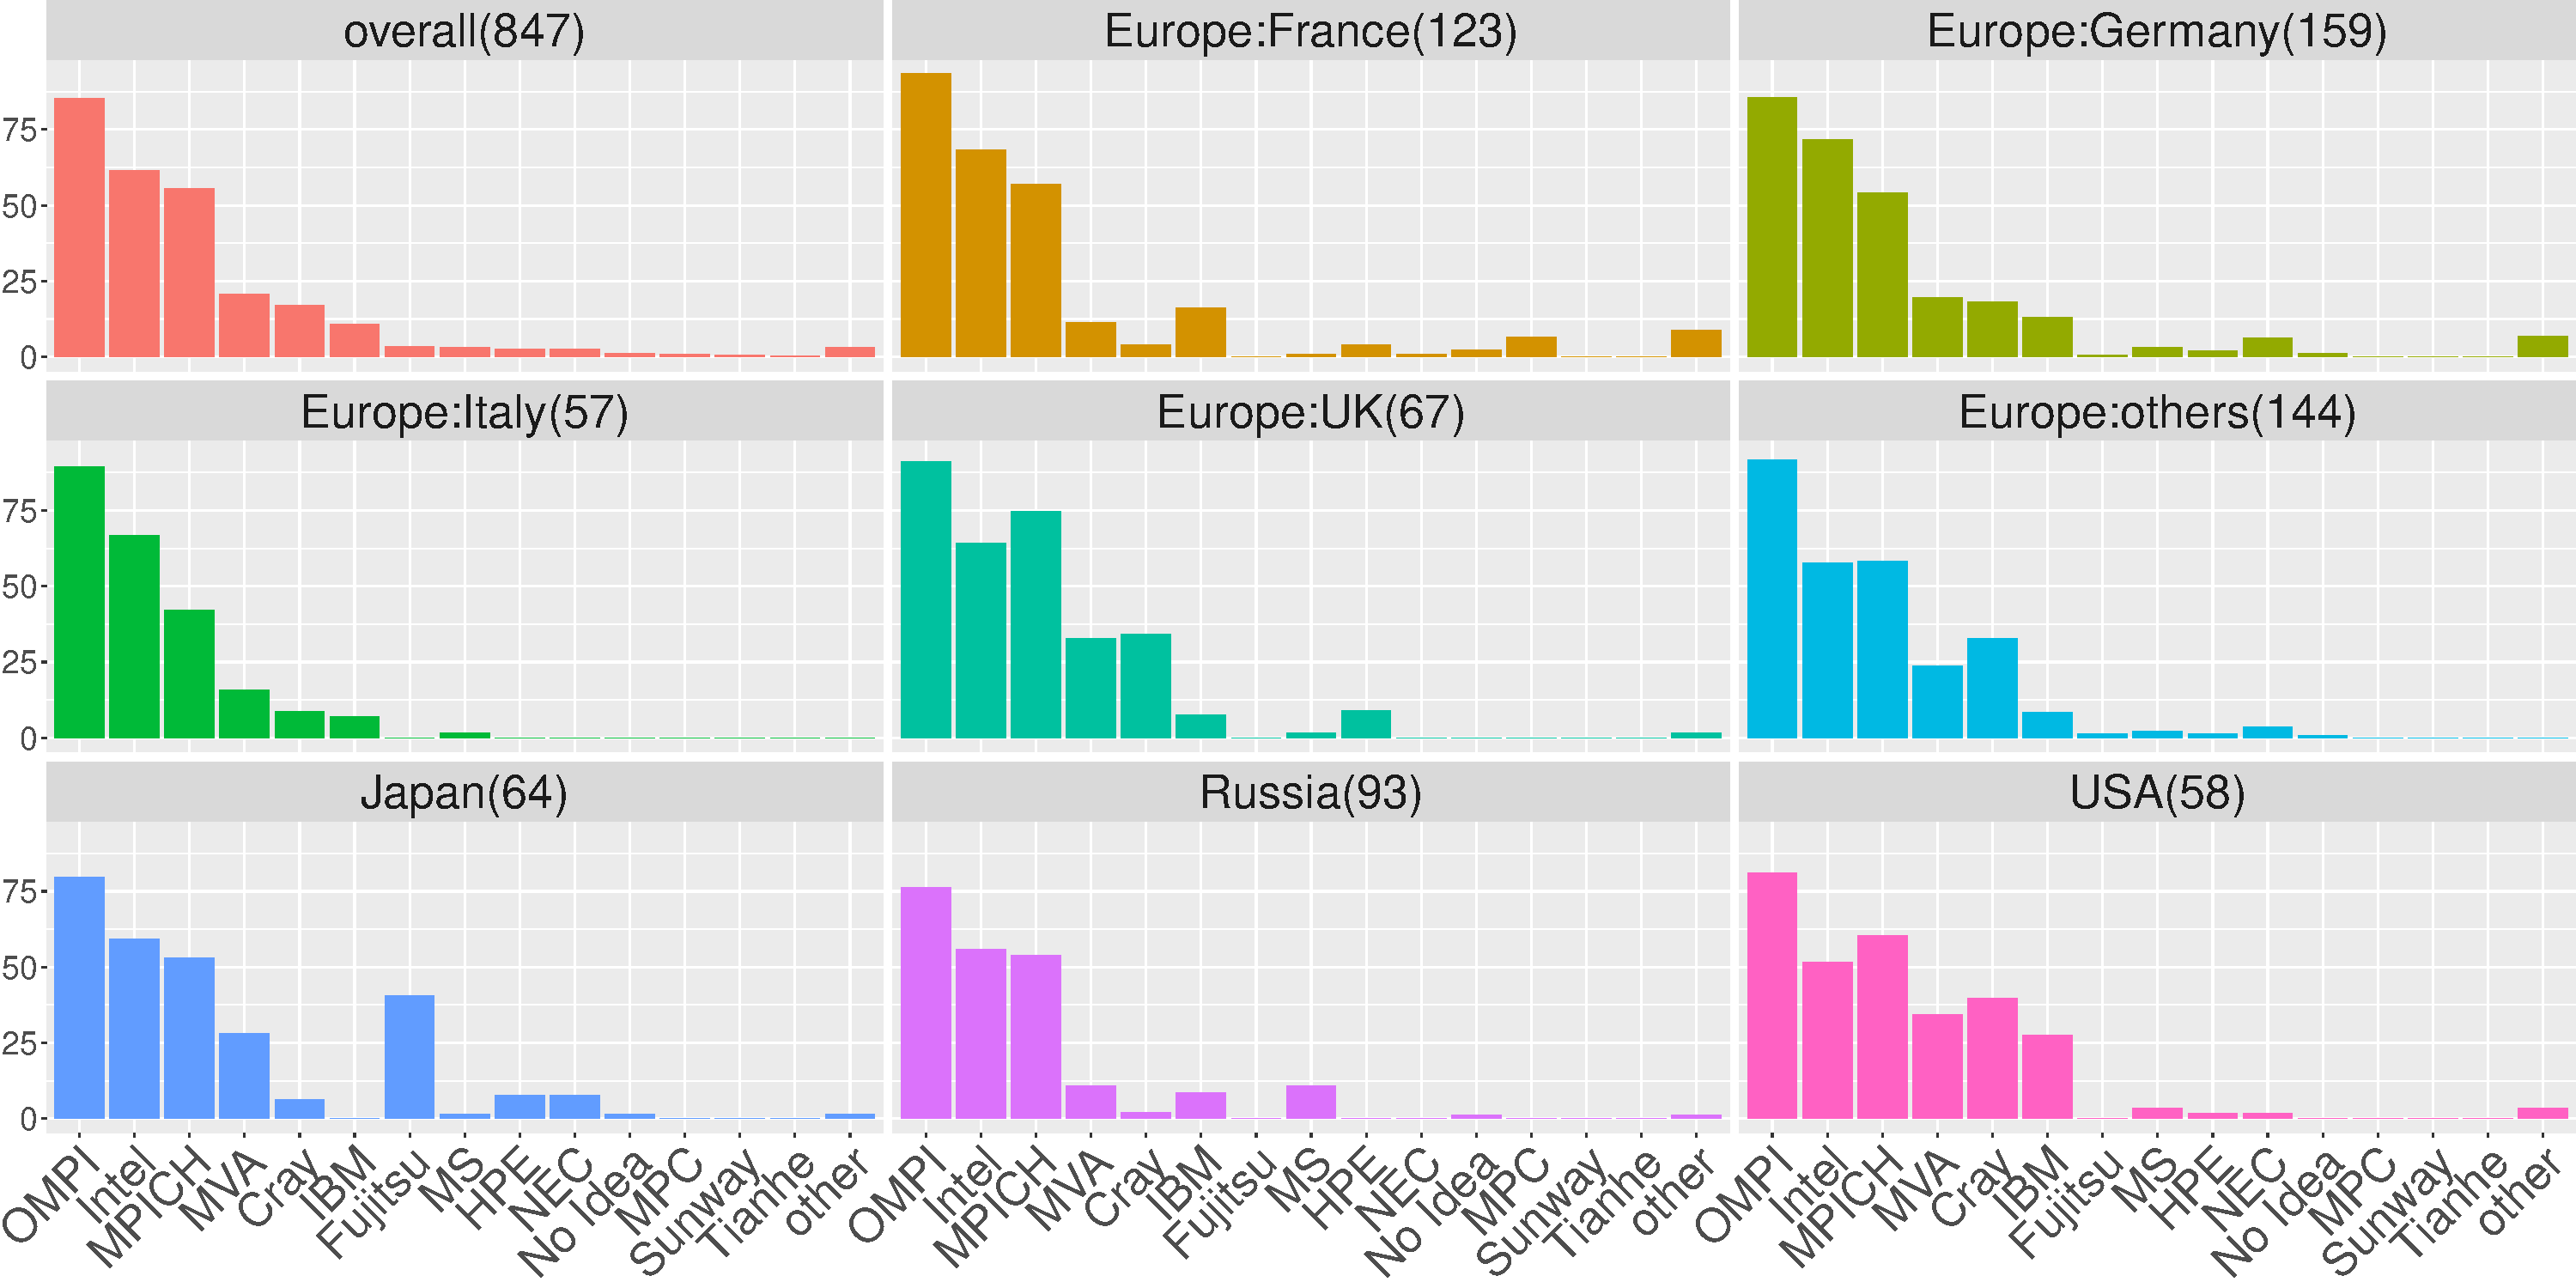
\includegraphics[width=8.7cm]{R-scripts/Q12.pdf}
      \caption{Q12: Using MPI Implementations {\it(multiple)}}
      \label{fig:using-implementations}
    \end{center}
  \end{figure}

  Q13 is asking \myquote{why did you choose the MPI implementation(s)} and its
  answers are shown in Fig.~\ref{fig:choosing-implementation}. The highest
  percentage of US participants selected \myquote{Familiar}. Many Italian
  participants also selected \myquote{Familiar.} Many Russian
  participants selected \myquote{No reason.} The largest part of UK and Germany
  participants selected \myquote{No choice.}
  In general, more than half of participants excepting US select MPI
  implementation(s) without any reason nor freedom of choice.

  \begin{figure}[htb]
    \begin{center}
      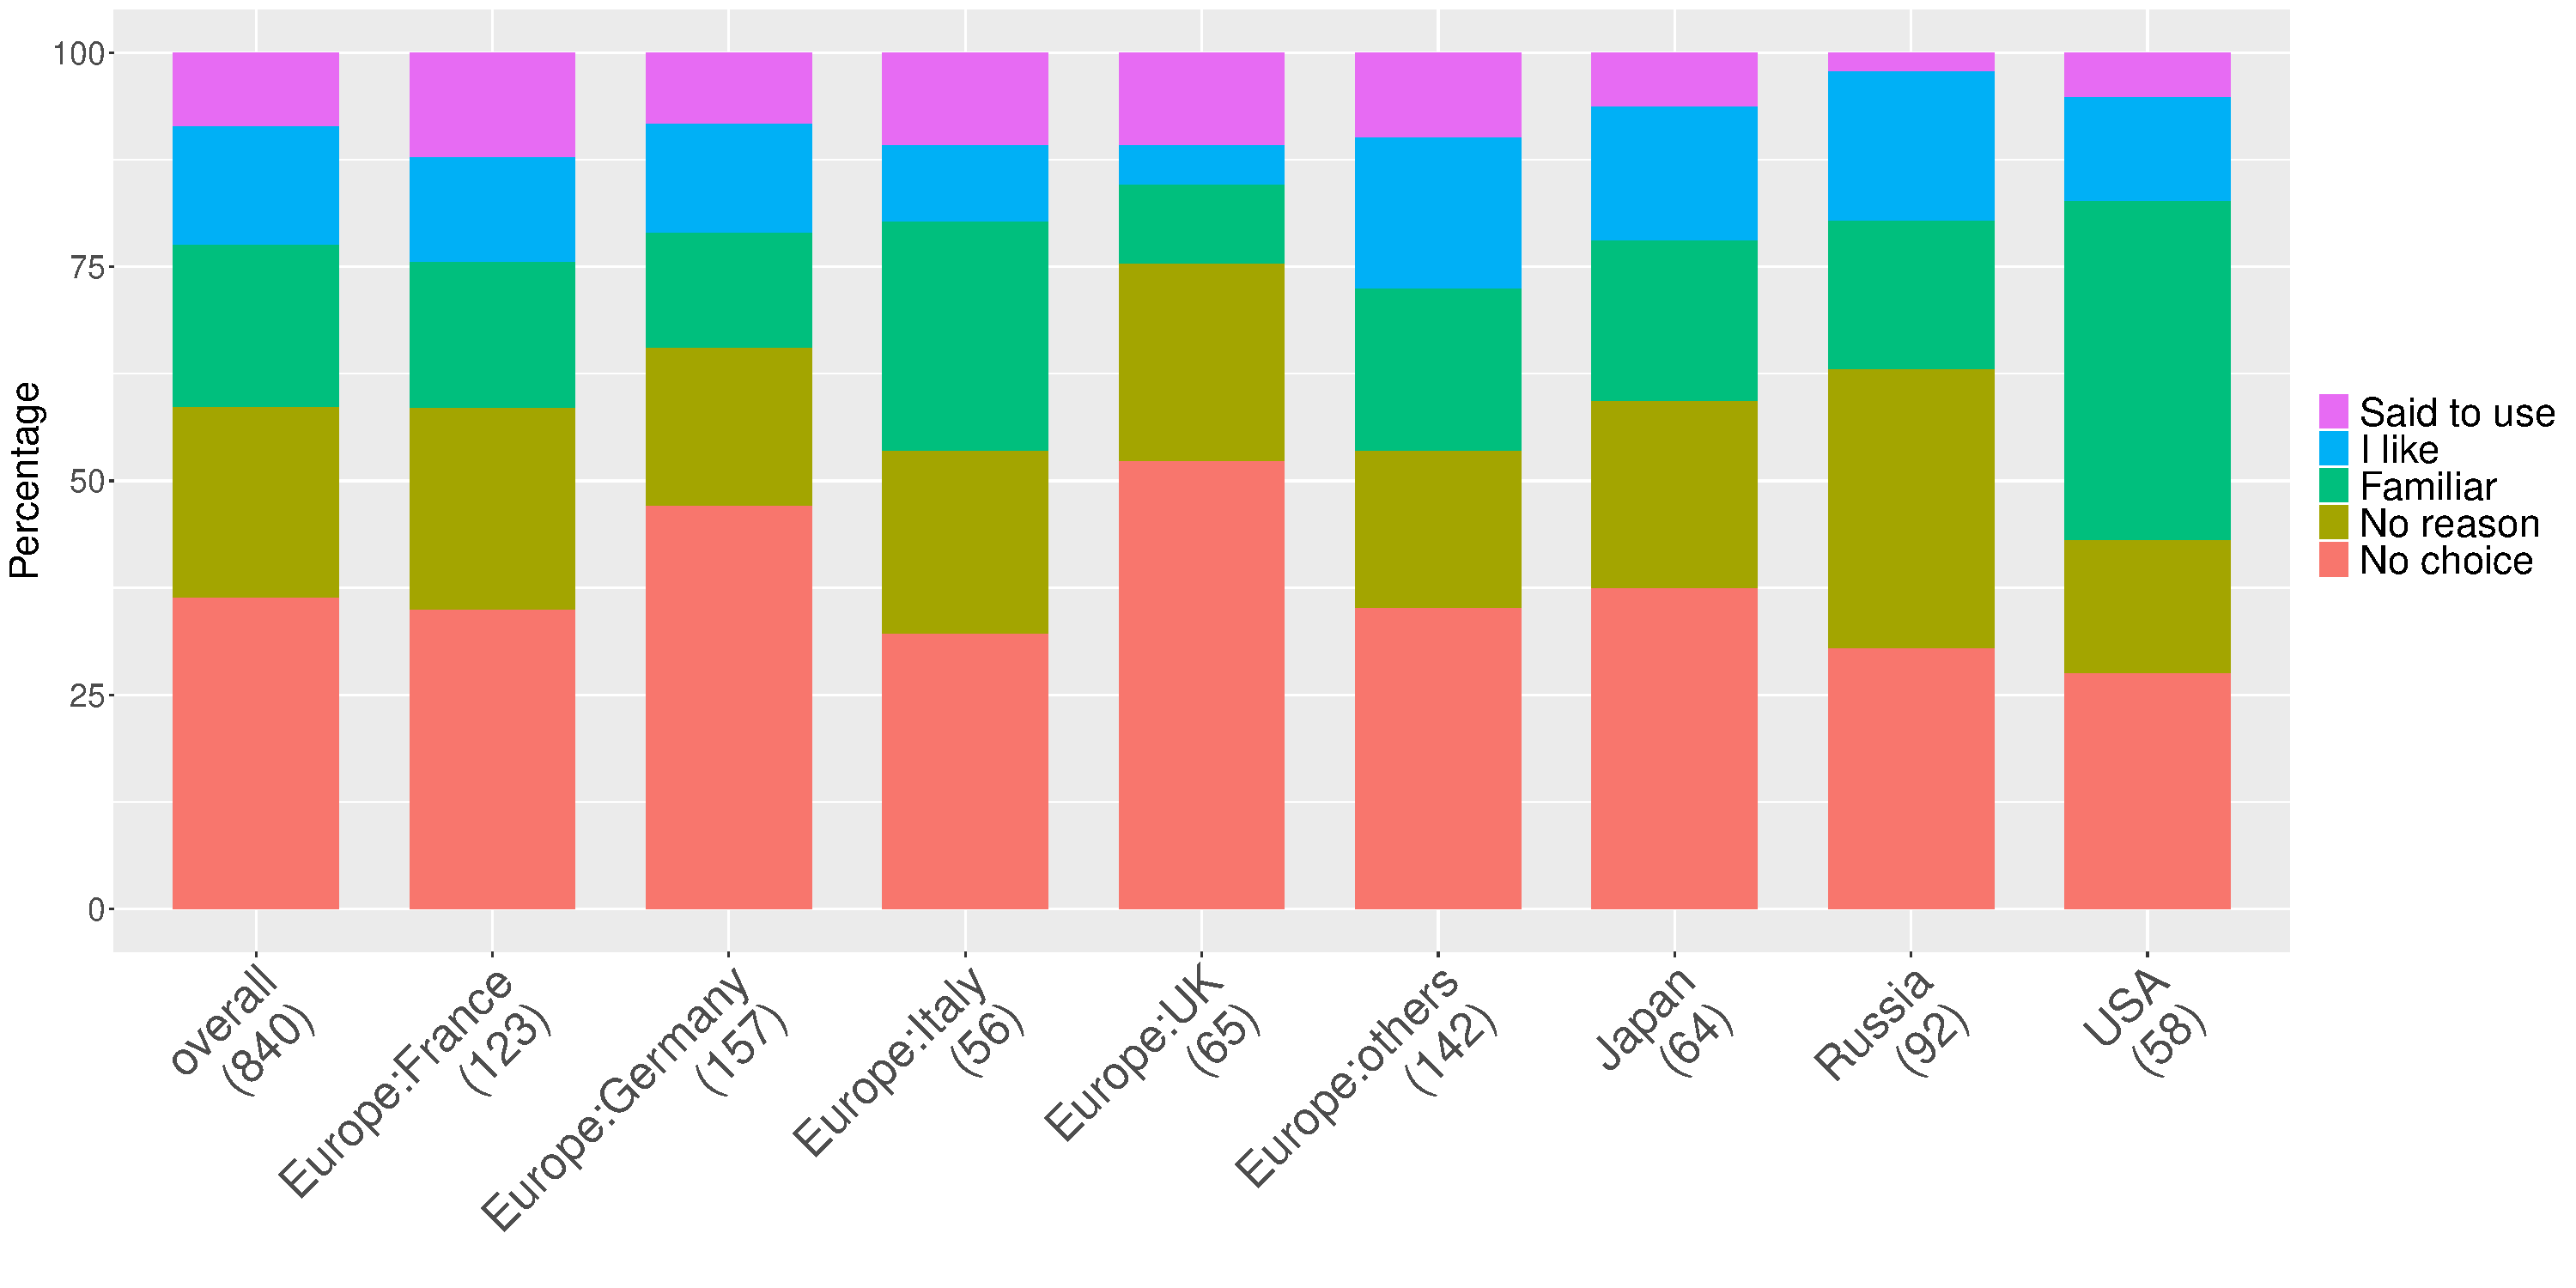
\includegraphics[width=8.7cm]{R-scripts/Q13.pdf}
      \caption{Q13: Choosing MPI Implementations {\it(single)}}
      \label{fig:choosing-implementation}
    \end{center}
  \end{figure}

\subsection{MPI+X and Alternatives}

Fig.~\ref{fig:mpi-x} shows the result of Q22 asking \myquote{Have you ever
written MPI+''X'' programs?}. Most participants have the experiences of
writing MPI+OpenMP programs. In US, \myquote{CUDA} is the second
largest and the percentage of \myquote{No} is the lowest among the
others. Considering the low percentage of \myquote{No} in overall (approx.
25\%), 3/4 participants using MPI with something else.
\cite{10.1145/3295500.3356176} also reported that the approximately 3/4 of
the target programs use the hybrid model of MPI+OpenMP.

\begin{figure}[htb]
\begin{center}
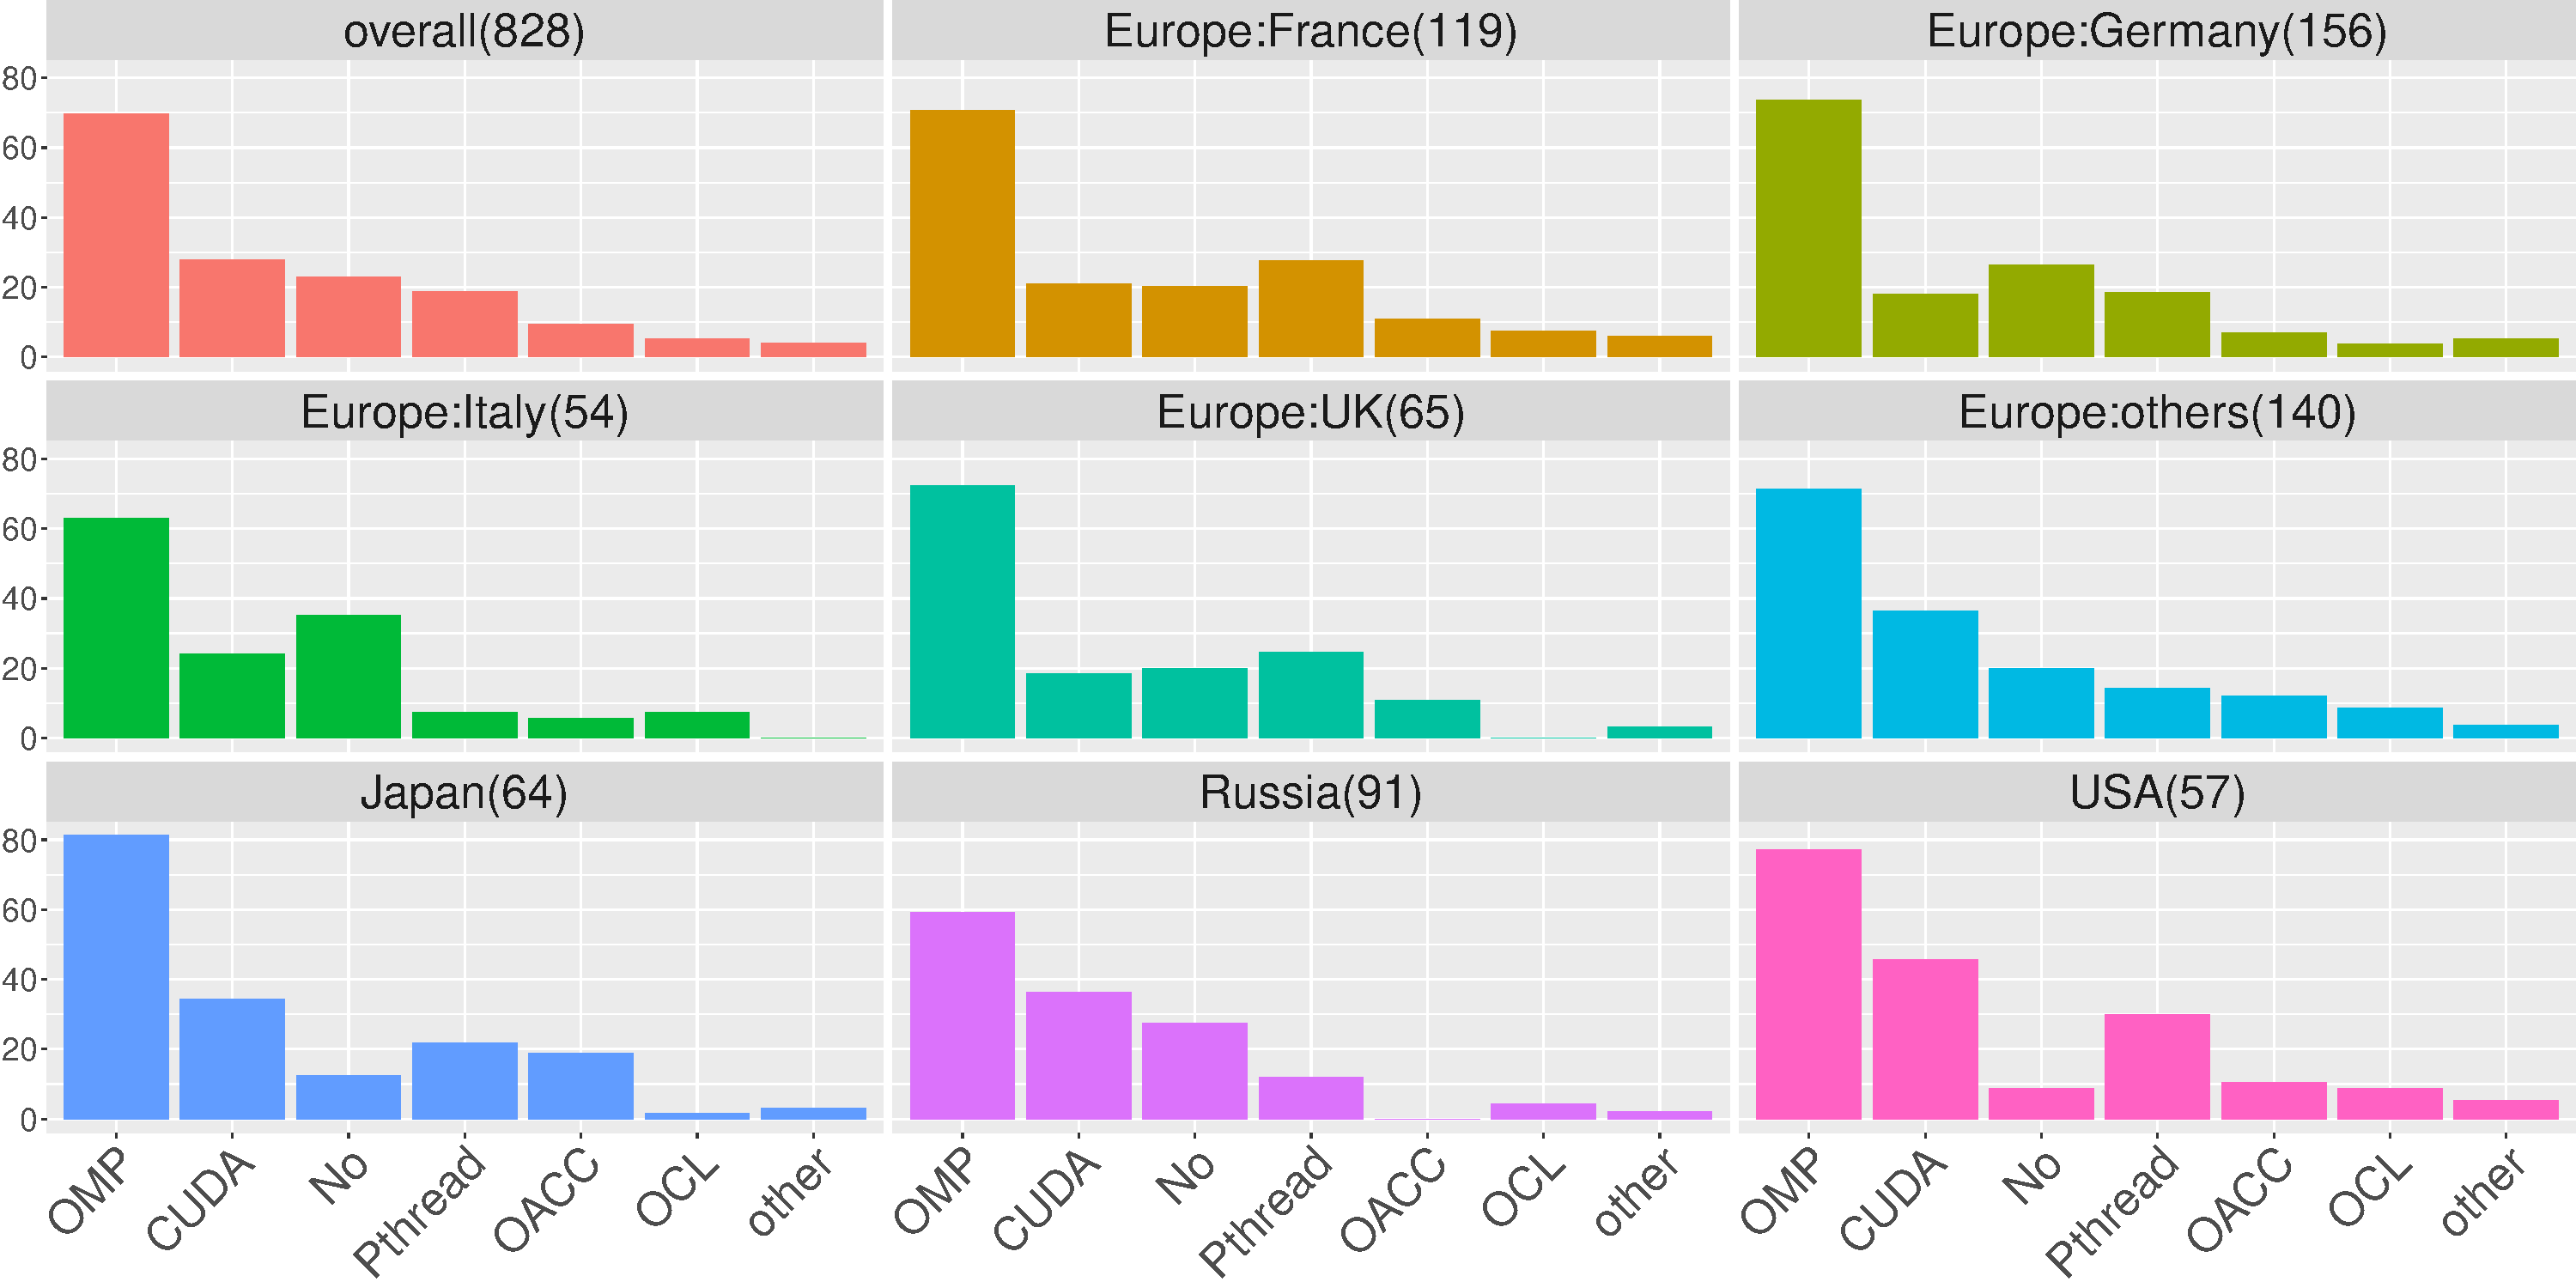
\includegraphics[width=8.7cm]{R-scripts/Q22.pdf}
\caption{Q22: MPI+X {\it(multiple)}}
\label{fig:mpi-x}
\end{center}
\end{figure}

\begin{figure}[htb]
\begin{center}
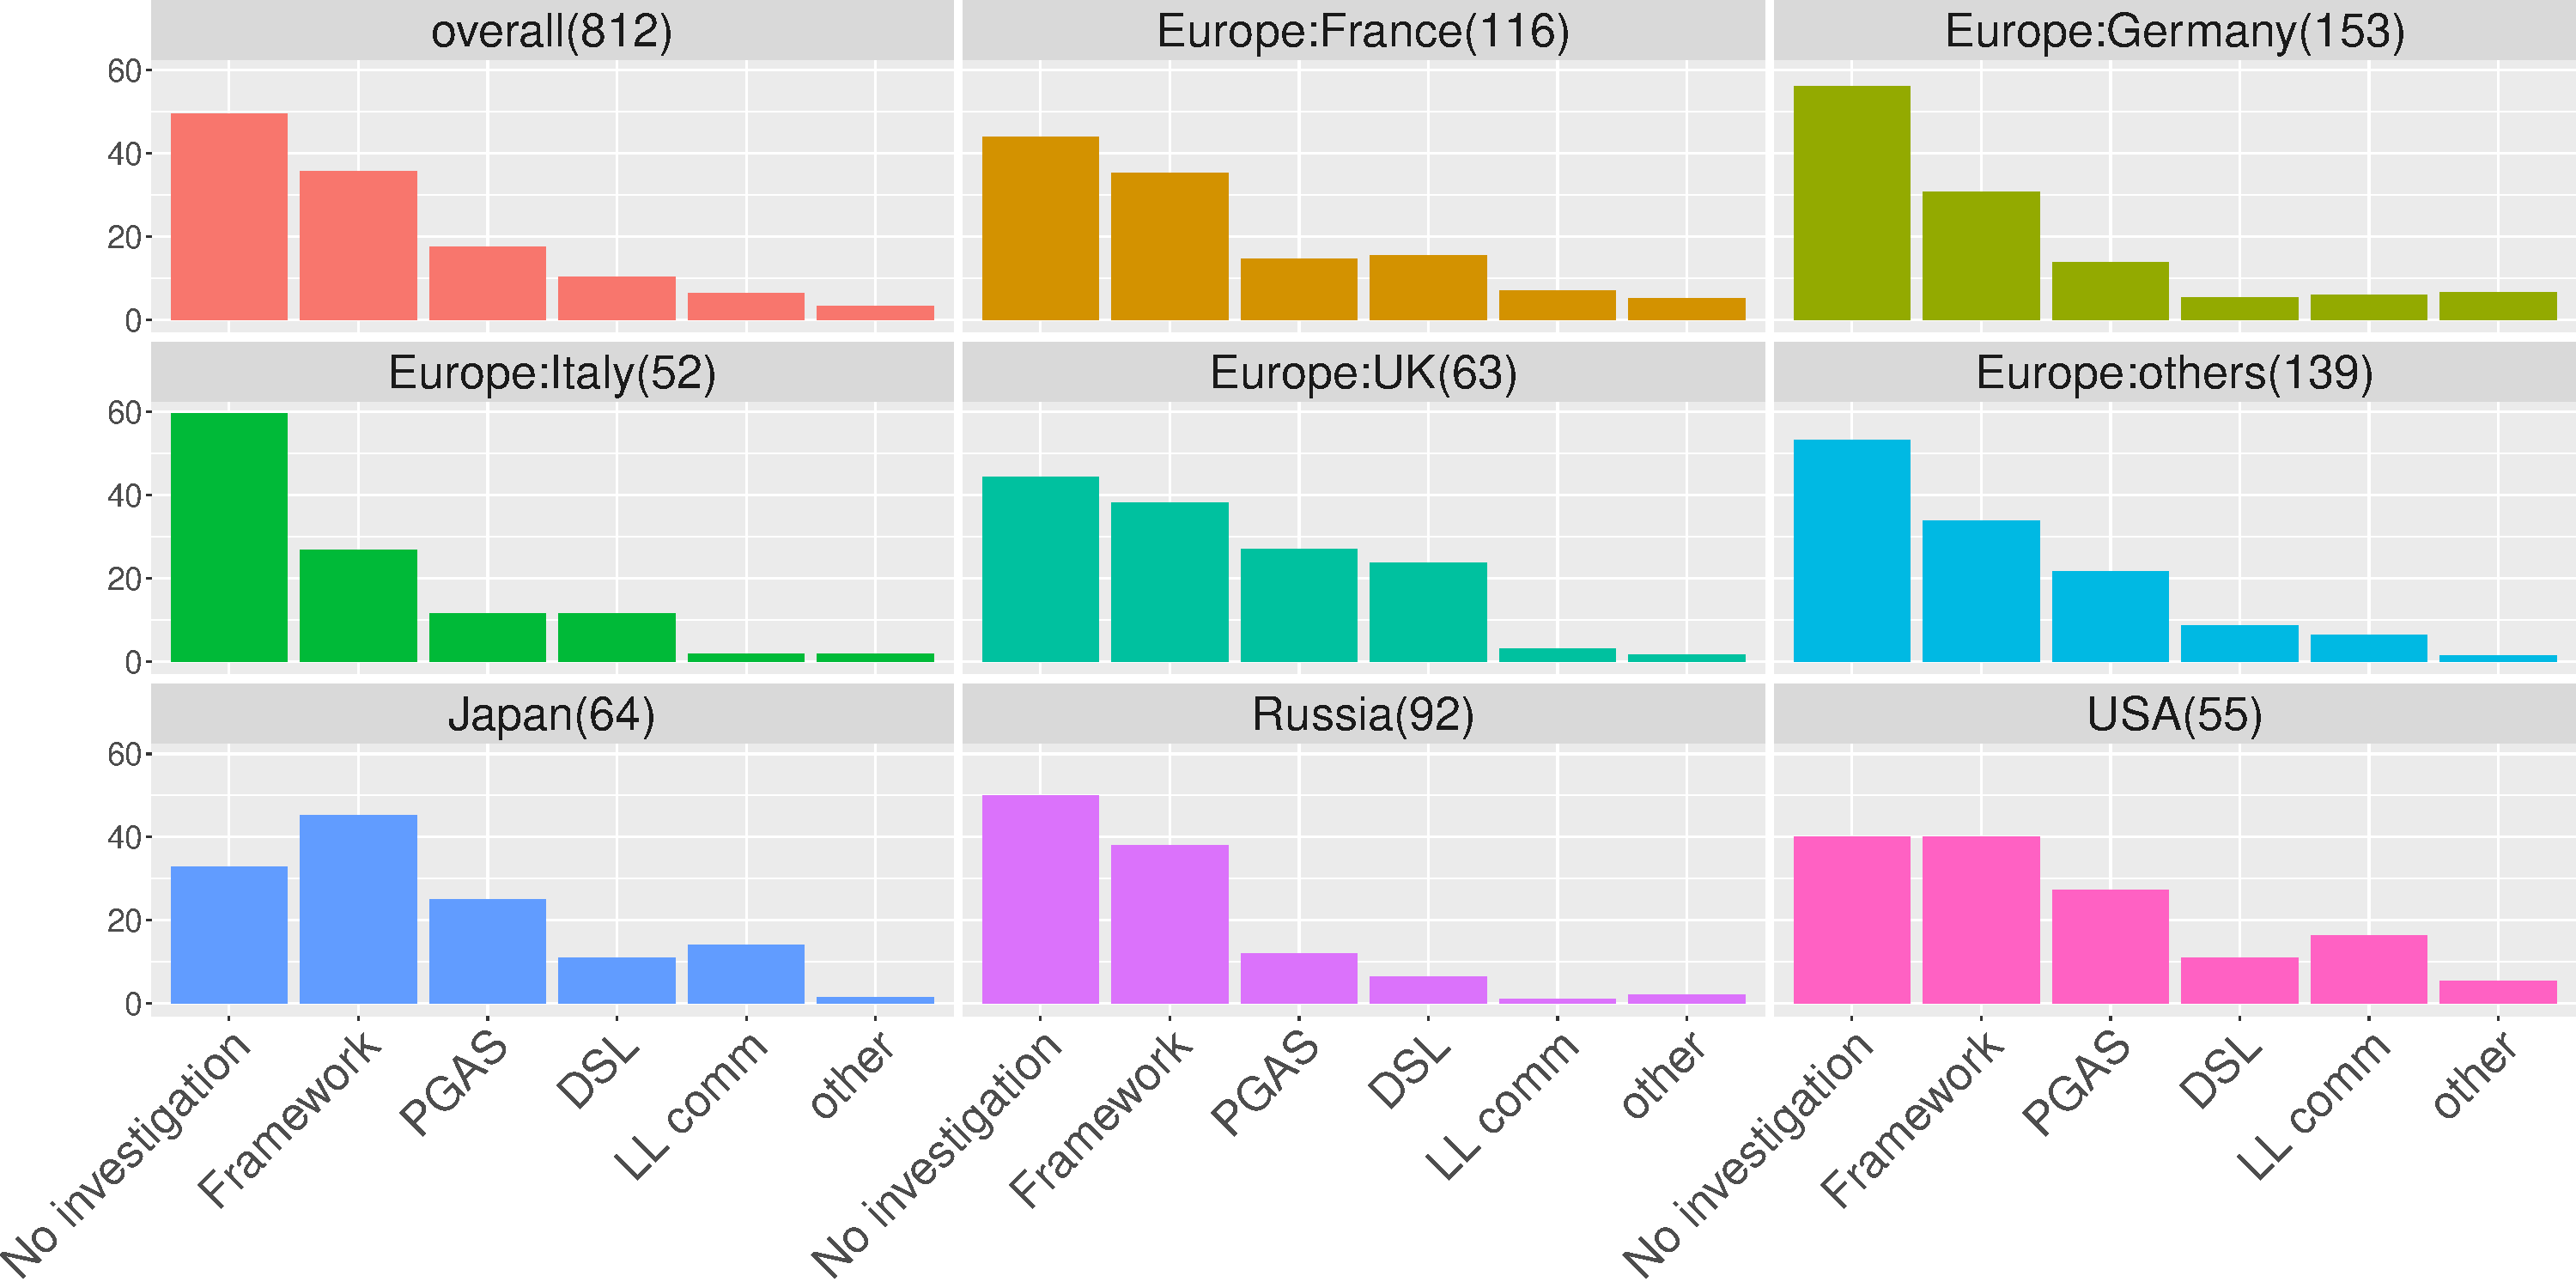
\includegraphics[width=8.7cm]{R-scripts/Q24.pdf}
\caption{Q24: MPI Alternatives {\it(multiple)}}
\label{fig:mpi-alternatives}
\end{center}
\end{figure}

When the participants were asked the question \myquote{What, if any,
alternatives are you investigating to indirectly call MPI or another
communication layer by using another parallel language~/ library?}, they
exhibited as shown in Fig.~\ref{fig:mpi-alternatives}. In overall,
almost half participants do not investigate the alternatives. The second
largest answer was \myquote{Framework} (i.e. a framework or library
using MPI) followed by \myquote{PGAS}. The
differences over the countries and regions are not so big.

\begin{figure}[htb]
\begin{center}
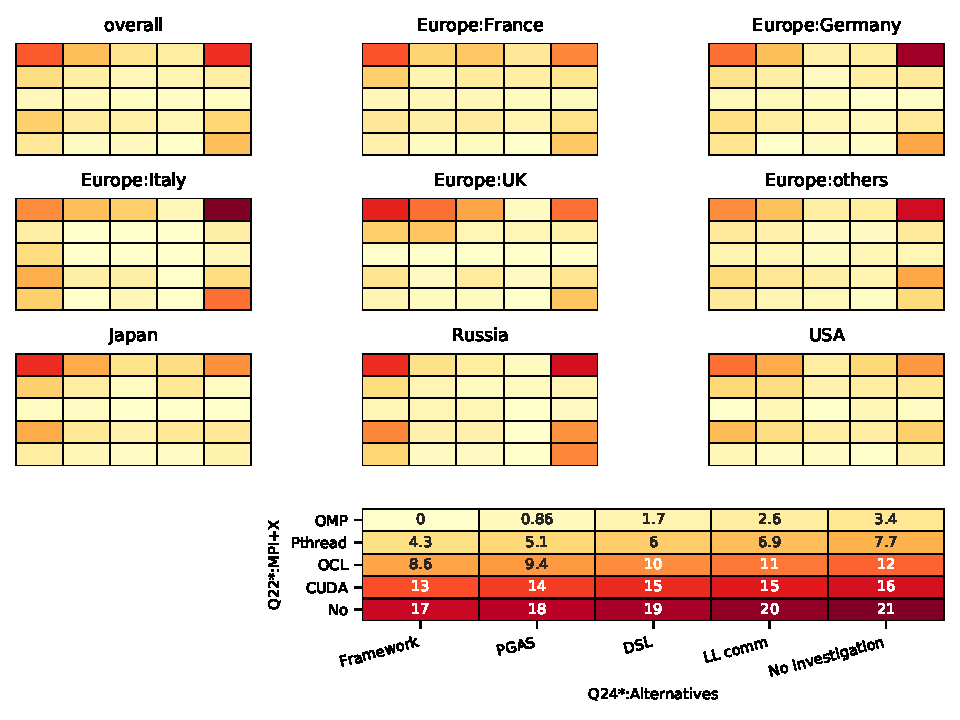
\includegraphics[width=8.7cm]{Figs/Q22-Q24.pdf}
\caption{Q22-Q24: MPI+X {\it(multiple)} and MPI Alternatives {\it(multiple)}}
\label{fig:mpi-x-and-alternatives}
\end{center}
\end{figure}

Fig.~\ref{fig:mpi-x-and-alternatives} shows the cross-tab analysis of
the above Q22 and Q24. A certain percentage of participants of
Germany, Italy, Russia and other European countries using MPI+OpenMP
without investigating the MPI alternative (upper right corners of the
heatmaps).

\subsection{Compatibility vs. Performance}

In somewhat long history of MPI, maintaining the backward
compatibility can be obstacles when introducing new features to
enhance MPI capabilities. Fig.~\ref{fig:performance-vs-compatibility}
shows the result of the question asking which is more important,
performance or compatibility. Fig.~\ref{fig:compatibility} shows the
percentages of Q28 asking backward compatibility.

\begin{figure}[htb]
\begin{center}
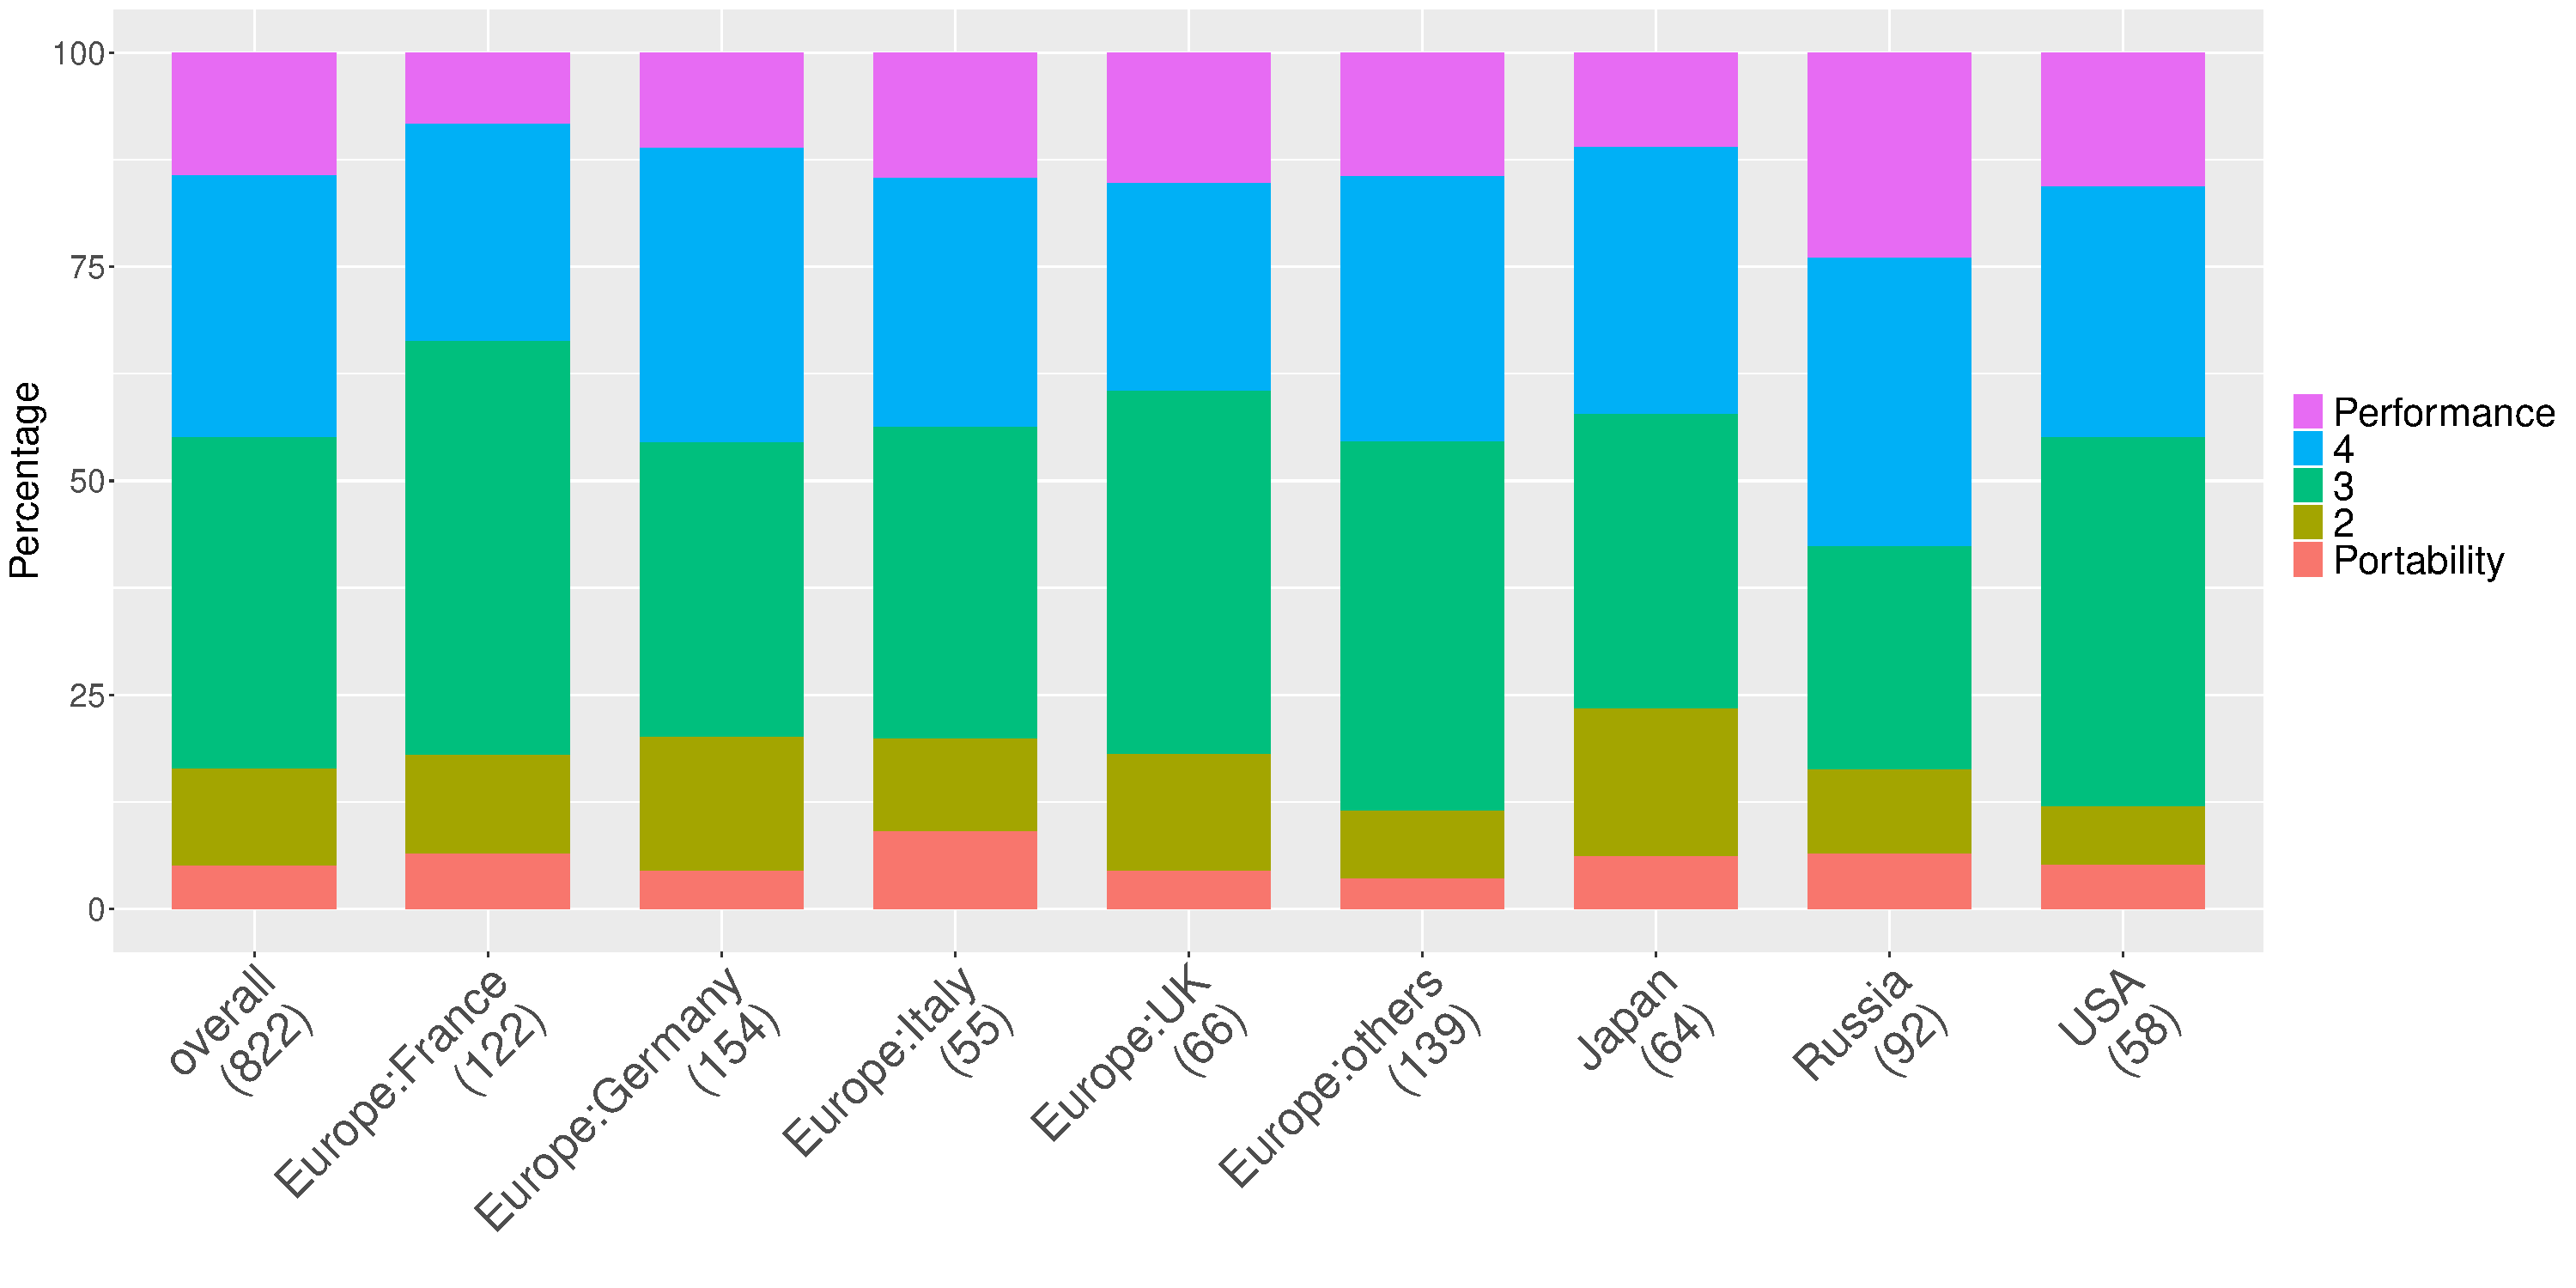
\includegraphics[width=8.7cm]{R-scripts/Q29.pdf}
\caption{Q29: Performance vs. Compatibility {\it(single)}}
\label{fig:performance-vs-compatibility}
\end{center}
\end{figure}

In Fig~\ref{fig:performance-vs-compatibility}, let's consider three
groups; {\it performance group} choosing \myquote{Performance} or
\myquote{4}, {\it compatibility group} choosing \myquote{Portability} or
\myquote{2}), and {\it grey group} who chose \myquote{3}. Apparently the grey
group dominates in most countries and regions (excepting Russia),
however, the performance group occupies more percentage. Regarding to
Russia, a certain percentage of Russian participants answered
\myquote{my program is too small} in Q21
(Fig.~\ref{fig:layering-mpi-calls}). If program is small enough, then
the compatibility does not cause a big problem.

\begin{figure}[htb]
\begin{center}
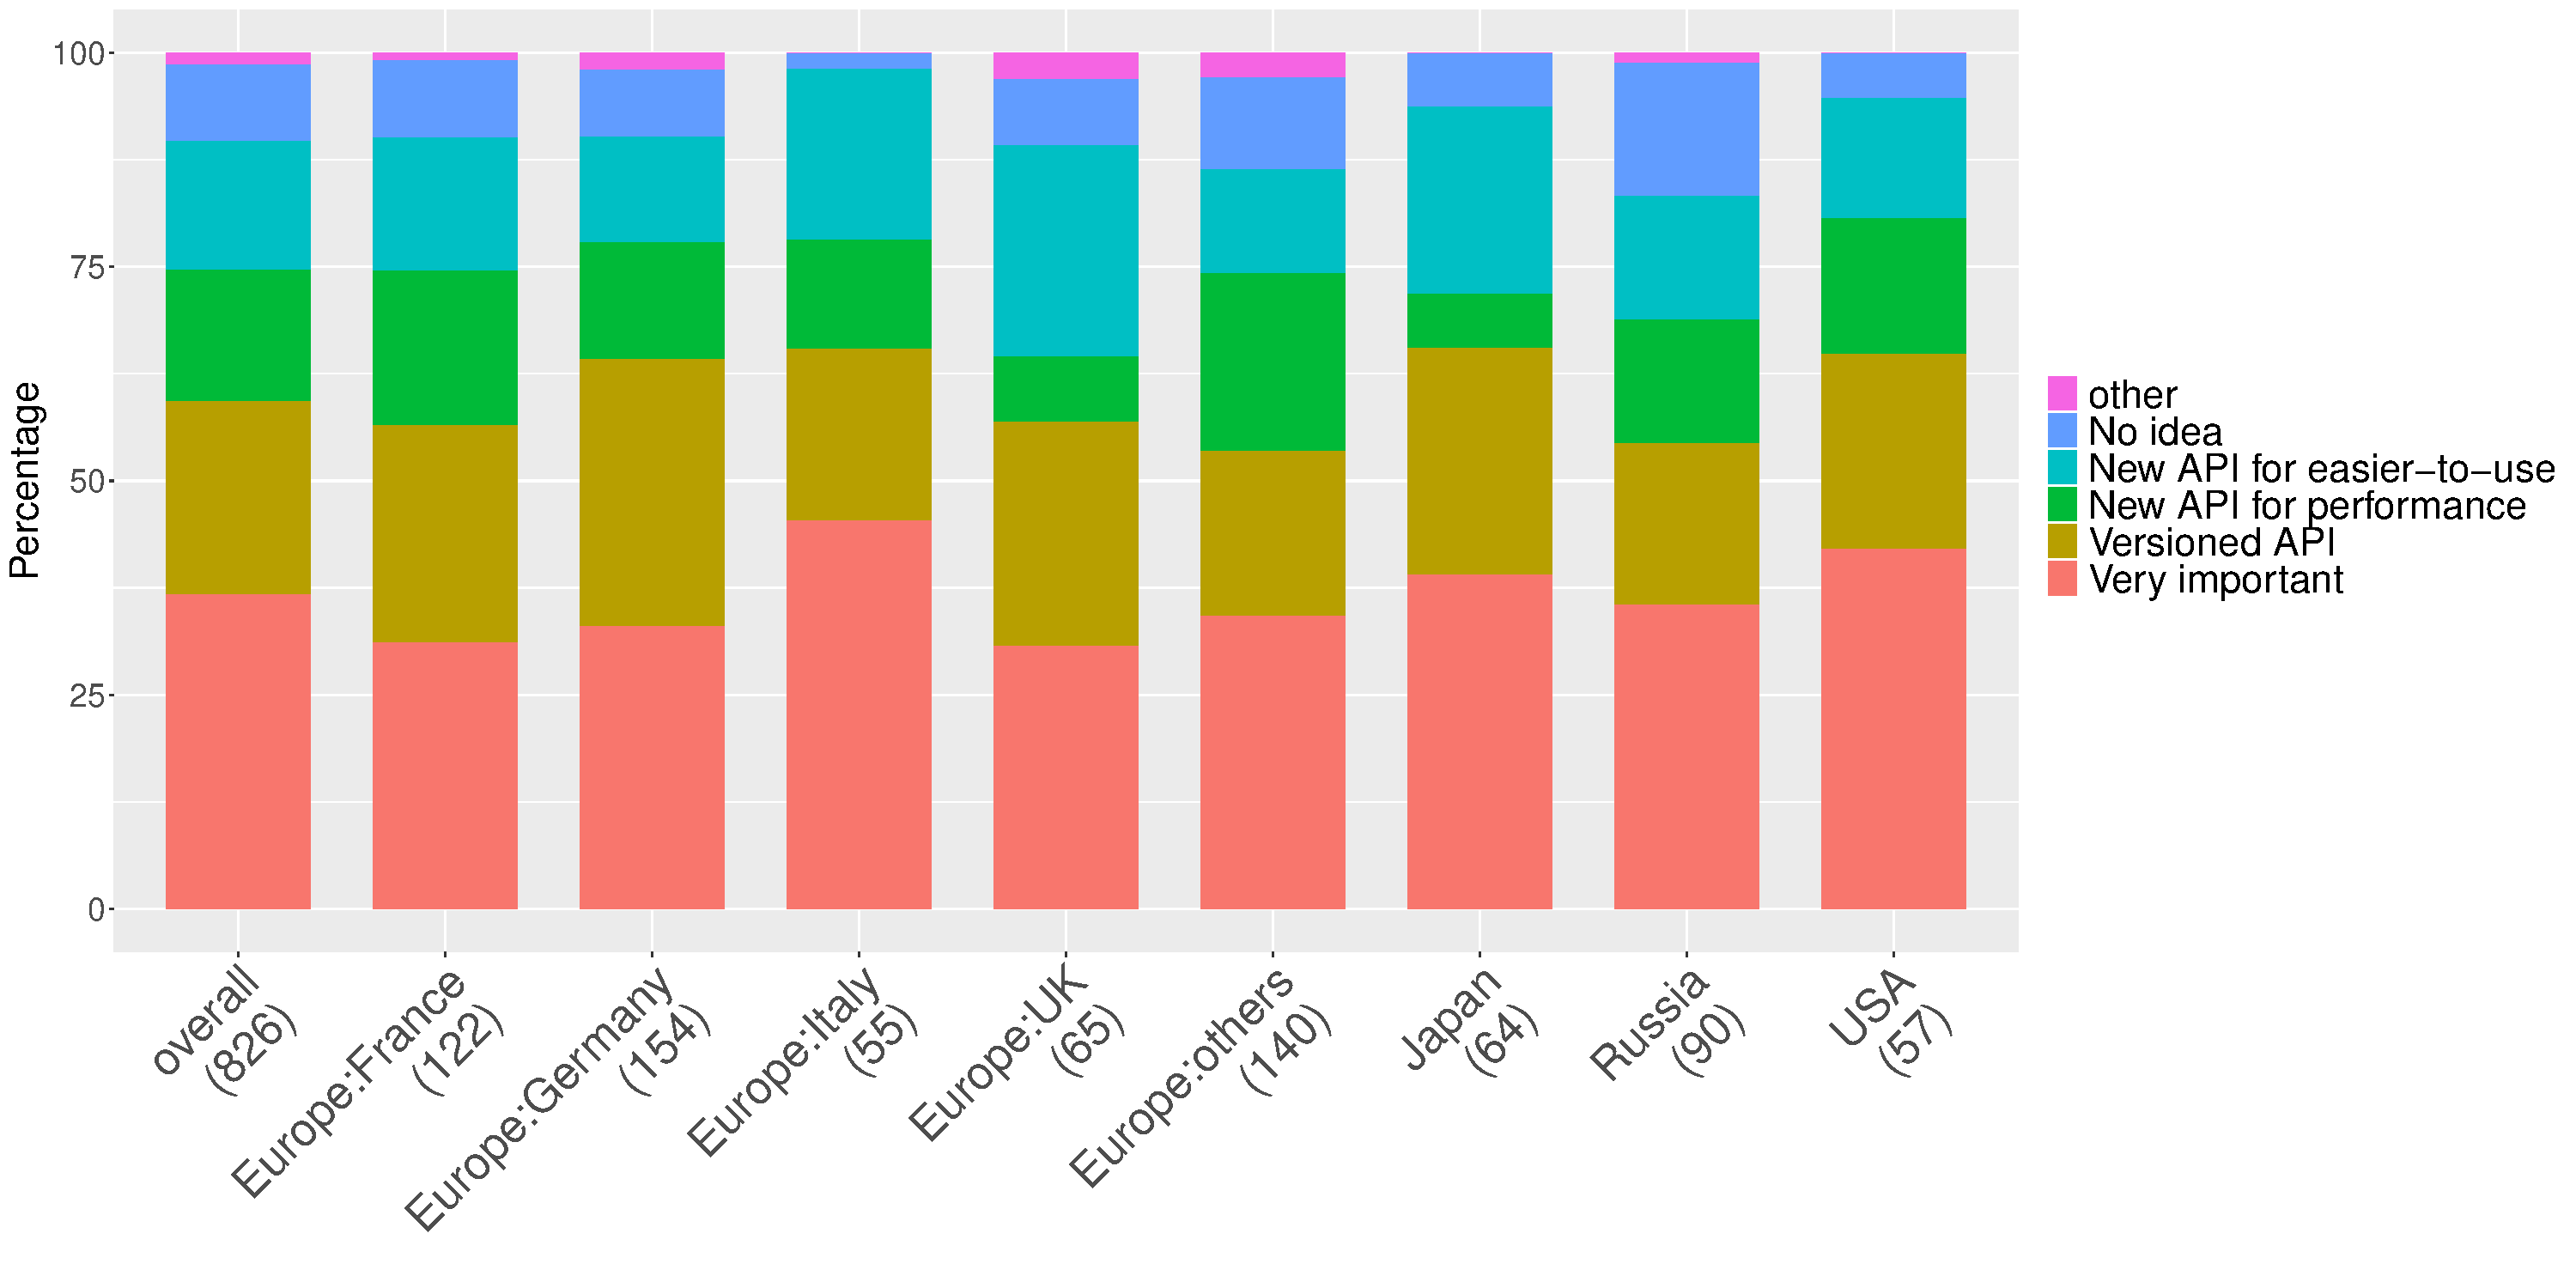
\includegraphics[width=8.7cm]{R-scripts/Q28.pdf}
\caption{Q28: Backward Compatibility {\it(single)}}
\label{fig:compatibility}
\end{center}
\end{figure}

As shown in Fig.~\ref{fig:compatibility}, around 40\% of participants
answered that the compatibility is very important, while the rest of
participants may accept the incompatibility conditionally. The
incompatibility forces users to update their programs. The result of
Q28 may suggests that users would accept incompatibility if the users
could get some kind of benefit from the incompatible updates of MPI
specification.

\subsection{Learning MPI}\label{sec:learning-mpi}

Fig.~\ref{fig:learning-mpi} shows the percentages of how participants
learned MPI. In this graph, \myquote{Other lec.} indicates the choice
\myquote{Other lectures or tutorials (workplace, conference)}. The
UK and Russia participants preferred to learn by Internet. The
participants of Germany and other European countries preferred to have
other lectures. The percentage of reading \myquote{Books} in US is the
highest. Taking a look at the other answers, 18 participants learned
by reading existing code and 8 participants learned by
doing\footnote{One participant answered \myquote{reverse engineering!}}.

\begin{figure}[htb]
\begin{center}
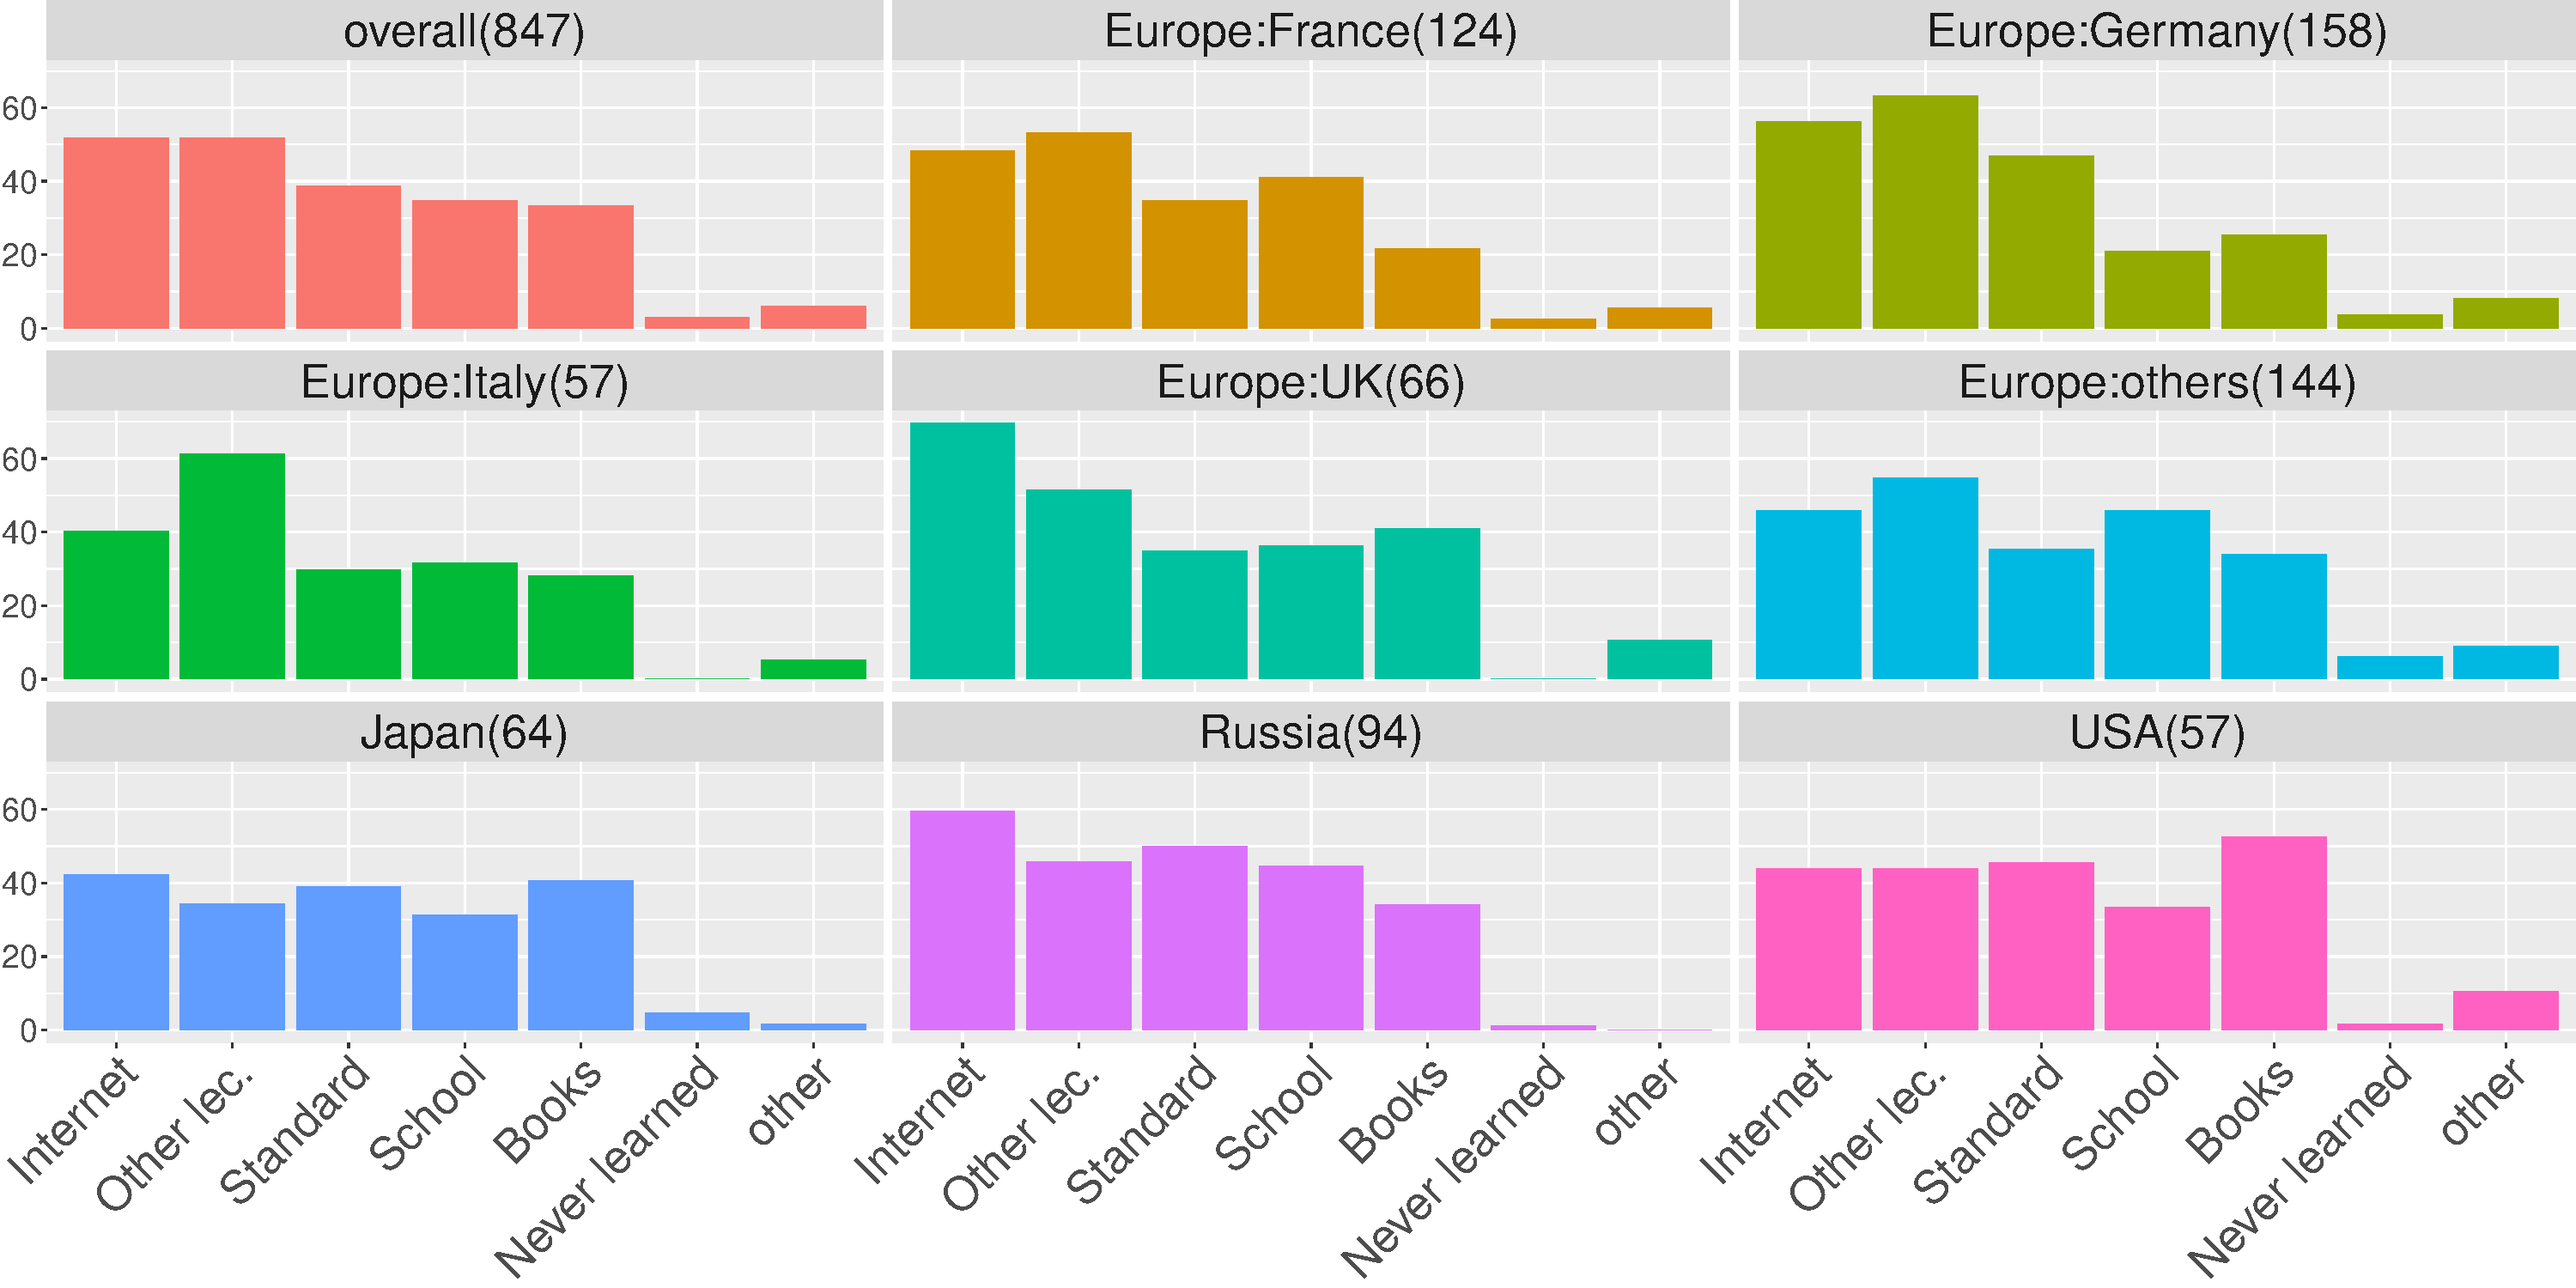
\includegraphics[width=8.7cm]{R-scripts/Q10.pdf}
\caption{Q10: Learning MPI {\it(multiple)}}
\label{fig:learning-mpi}
\end{center}
\end{figure}

Fig.~\ref{fig:reading-standard} shows the graph of Q9, asking if
participants have read the MPI standard document. Not surprisingly,
around 60\% of participants, independent from countries, read the
standard partly. Most interesting country is UK, where the percentage
of participants reading all document and, at the same time, the
percentage of the answer \myquote{No} are the highest among the
countries and regions.

\begin{figure}[htb]
\begin{center}
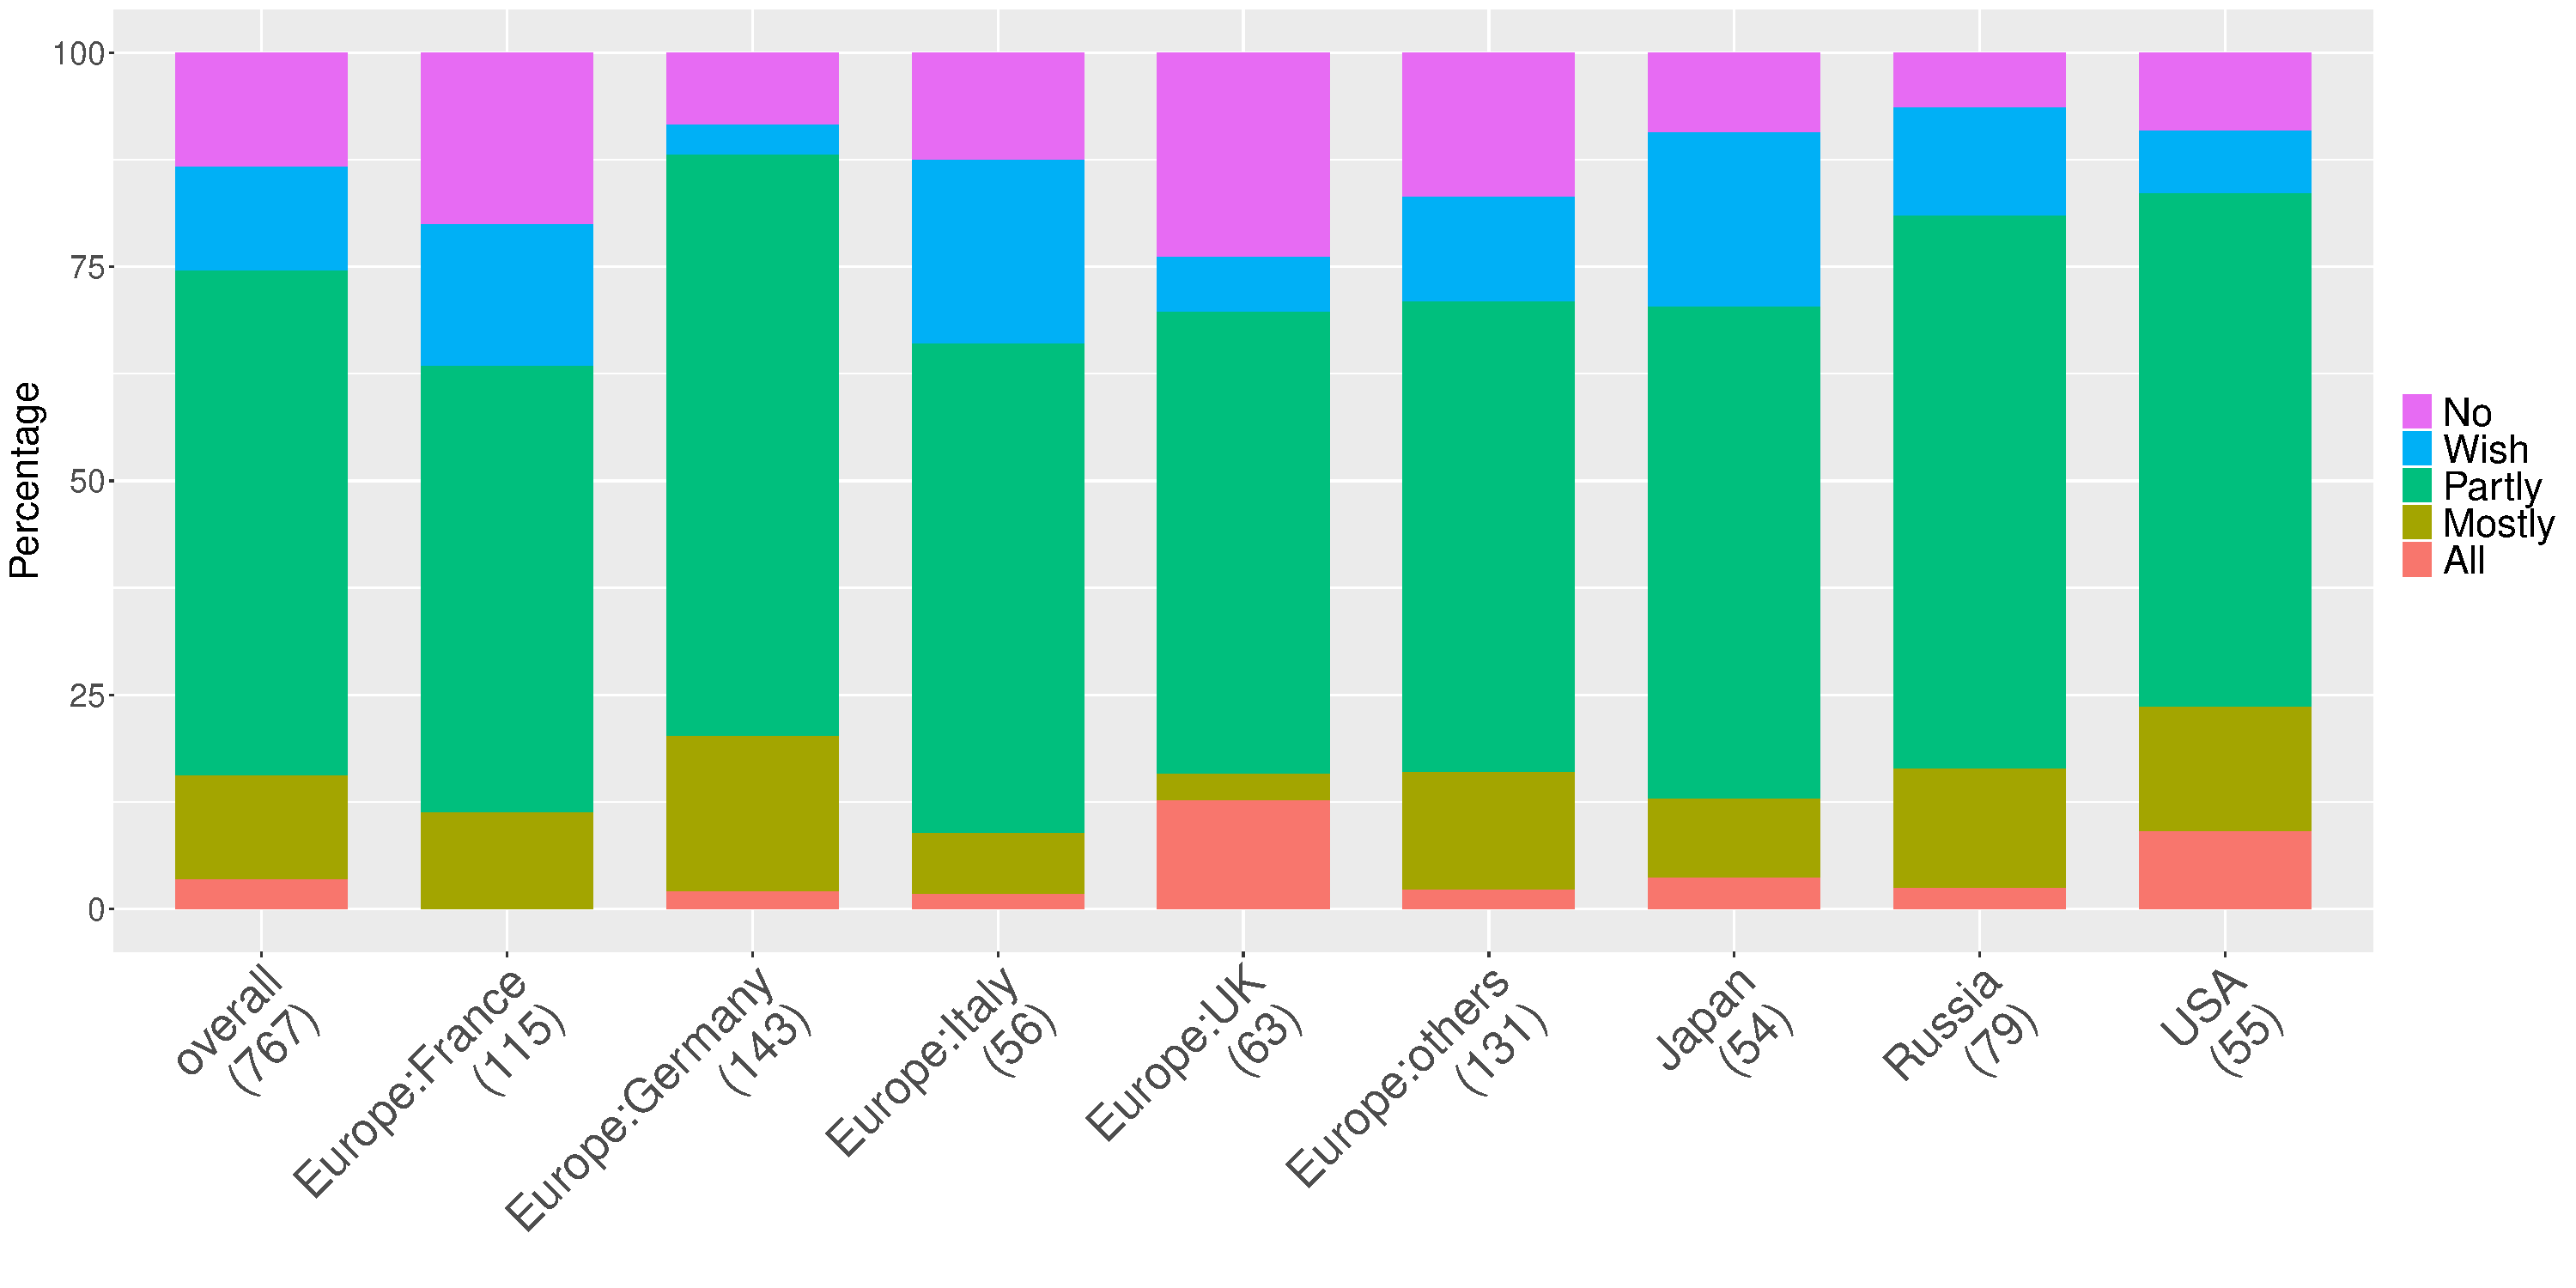
\includegraphics[width=8.7cm]{R-scripts/Q9.pdf}
\caption{Q9: Reading MPI Standard {\it(single)}}
\label{fig:reading-standard}
\end{center}
\end{figure}

Now let's see how people are writing MPI
programs. Fig.~\ref{fig:checking-spec} shows the percentages of Q14
asking \myquote{How do you check MPI specifications when your are writing MPI
programs?} Most users are checking MPI specifications by reading online
documentations (e.g., man pages), searching Internet, and reading the
standard. As shown in the previous figure
(Fig.~\ref{fig:reading-standard}), users are reading the standard
partly because of checking the MPI specifications.

\begin{figure}[htb]
\begin{center}
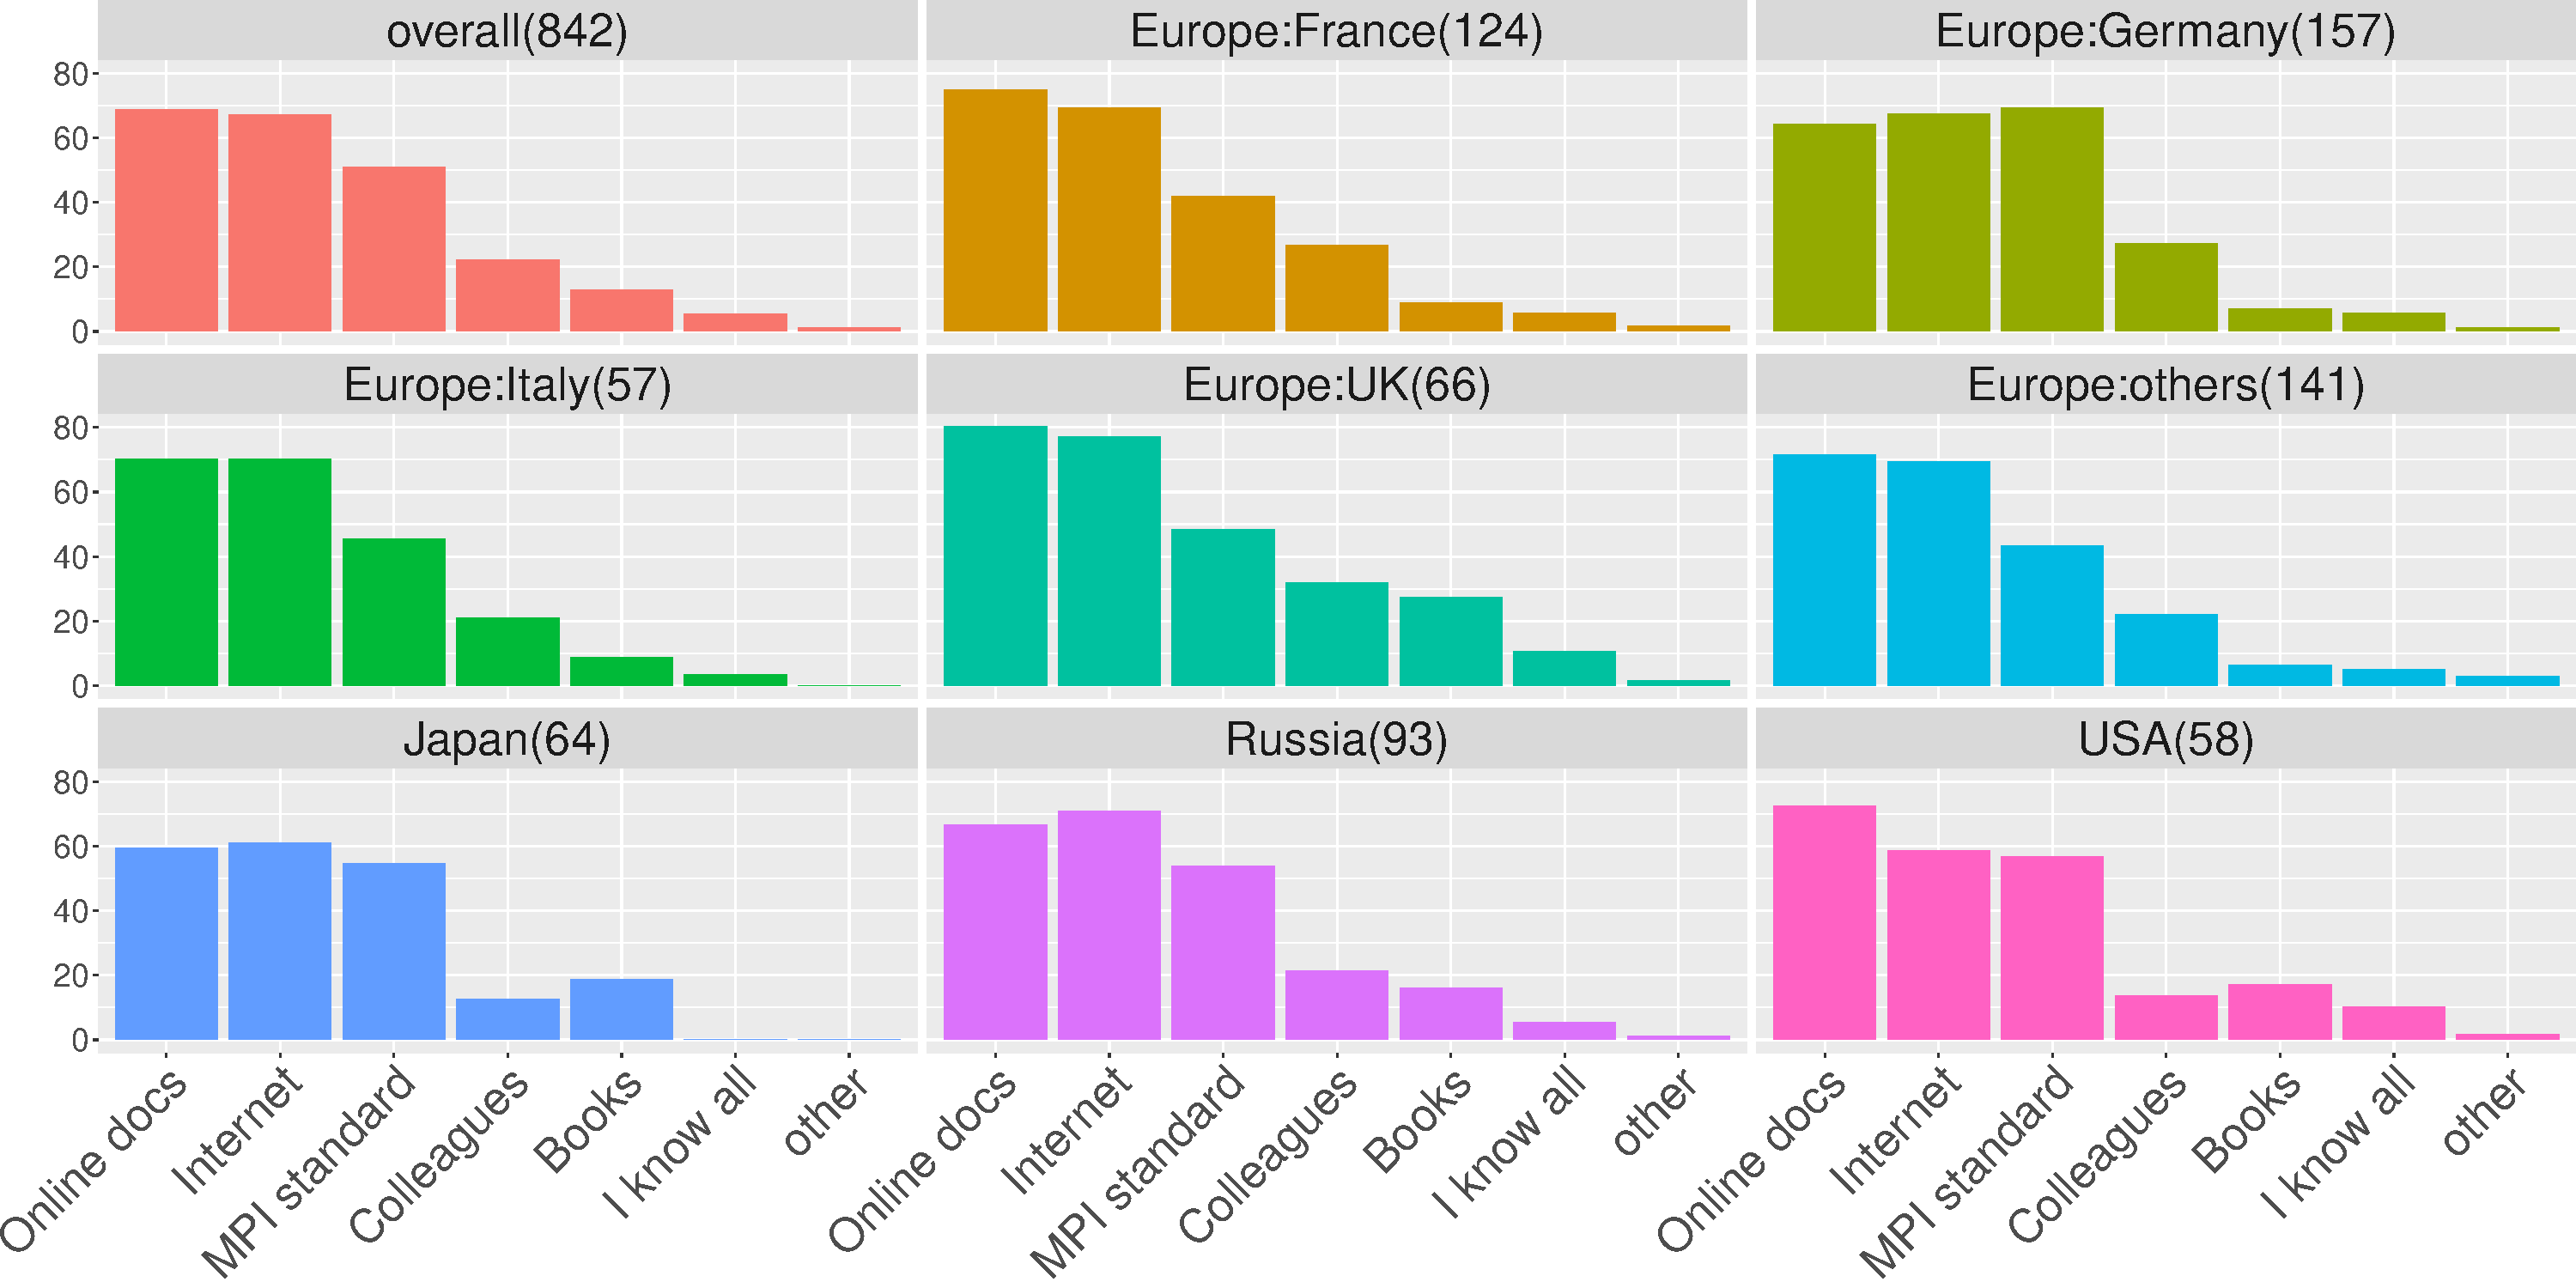
\includegraphics[width=8.7cm]{R-scripts/Q14.pdf}
\caption{Q14: Checking Specification {\it(multiple)}}
\label{fig:checking-spec}
\end{center}
\end{figure}

It would be nice to have the cross-tab analysis between Q3 (MPI skill)
and Q9 (reading MPI standard). Unfortunately the participants reading
the standard partly dominates the answer and the cross-tab analysis
between them did not give us any clear evidence.  Instead here we have
Fig.~\ref{fig:reading-standard-and-checking-spec}, cross-tab
heatmaps between Q3 and above Q14. There can be seen a a weak
correlation, those who check MPI standard have higher MPI skill,
between those two questions in some countries (France, Germany, and
Japan).

\begin{figure}[htb]
\begin{center}
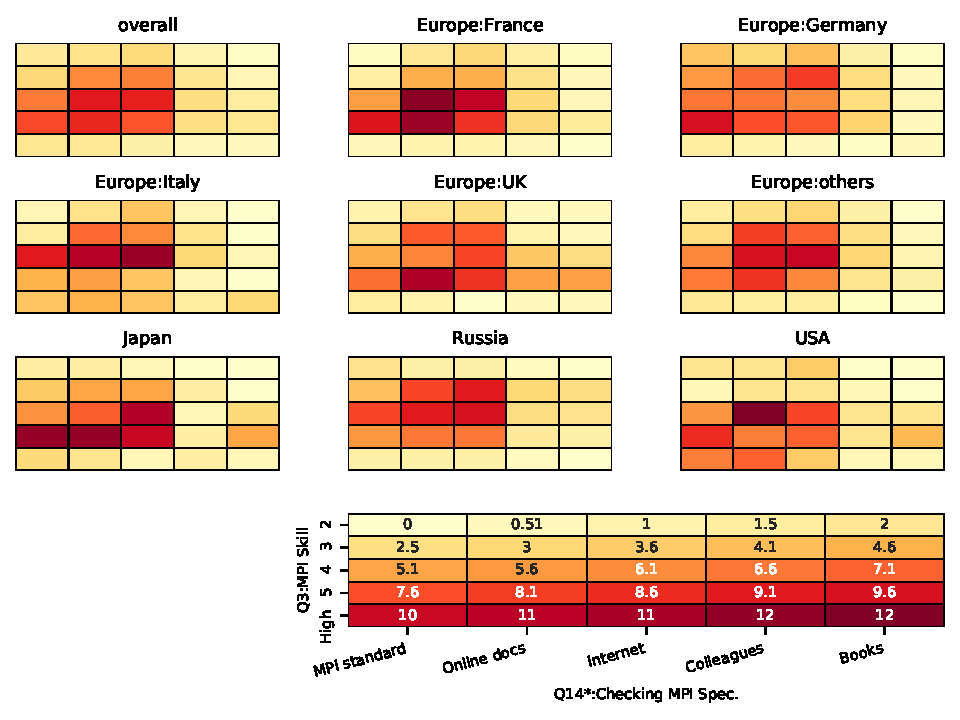
\includegraphics[width=8.7cm]{Figs/Q3-Q14.pdf}
\caption{Q3-Q14: MPI Skill {\it(single)} and Checking Specification {\it(single)}}
\label{fig:reading-standard-and-checking-spec}
\end{center}
\end{figure}

Another interesting result can be seen in Fig.~\ref{fig:prog-skill}
asking \myquote{Rate your overall programming skill (non-MPI
  programs)}. People with high programming skills who chose 4 or more
account for more than 90\%. This indicates that
people with high program skills shown interest in our survey and/or
that program beginners do not use MPI. This might indicate that MPI
programming requires specific skills whom basic developers do not
necessarily master. By country comparison, Russia shows a different
tendency from other countries.

\begin{figure}[htb]
\begin{center}
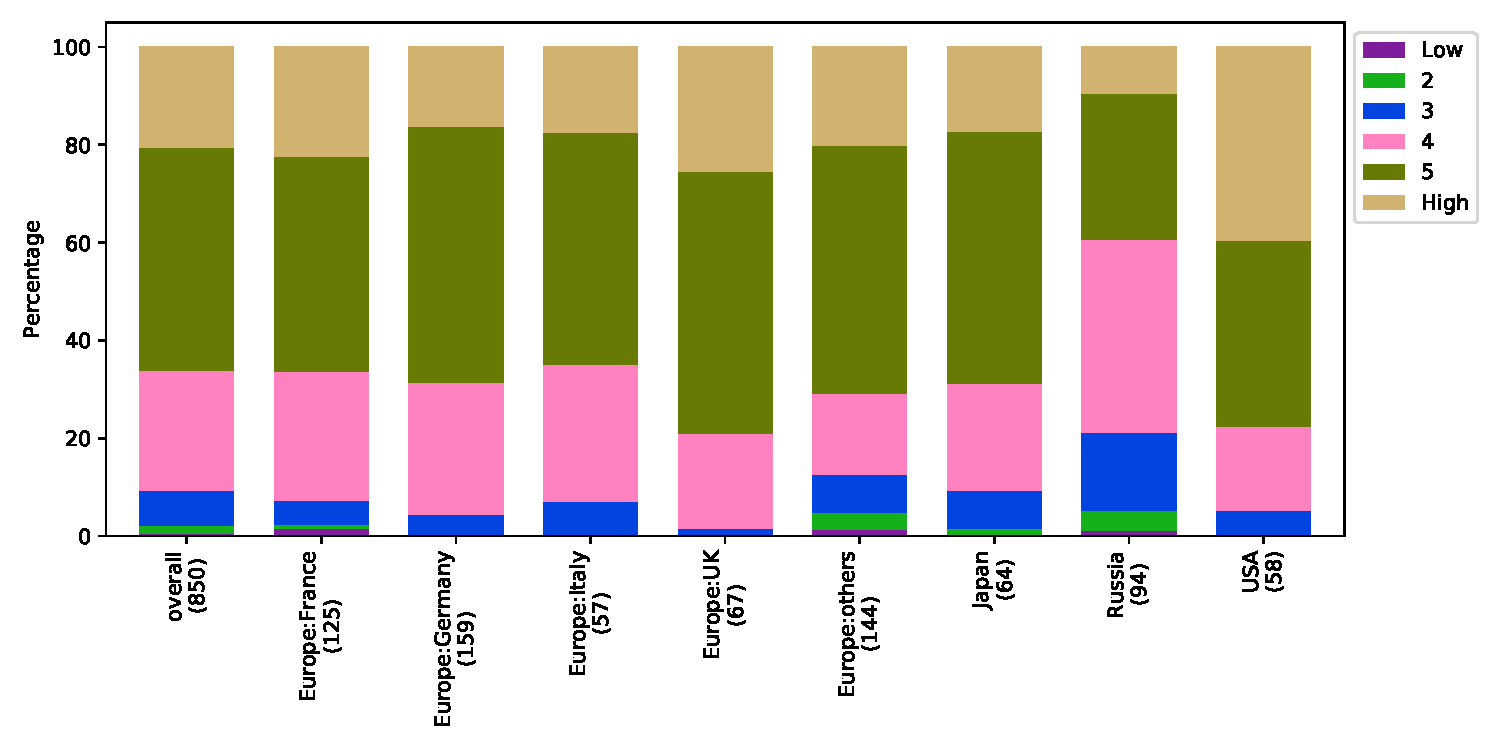
\includegraphics[width=8.7cm]{Figs/Q2.pdf}
\caption{Q2: Rate your overall programming skill (non-MPI
  programs)}
\label{fig:prog-skill}
\end{center}
\end{figure}

Generally speaking, there can be a case where a particular question in
a survey may ignite for participants to explode their dissatisfaction
by writing messages into a free text field. In our survey Q19 asking
\myquote{What are your obstables to mastering MPI?} is
such a question. The largest number of \myquote{other} inputs can be
found at Q19 (Fig.~\ref{fig:learning-obstacles}).

\begin{figure}[htb]
\begin{center}
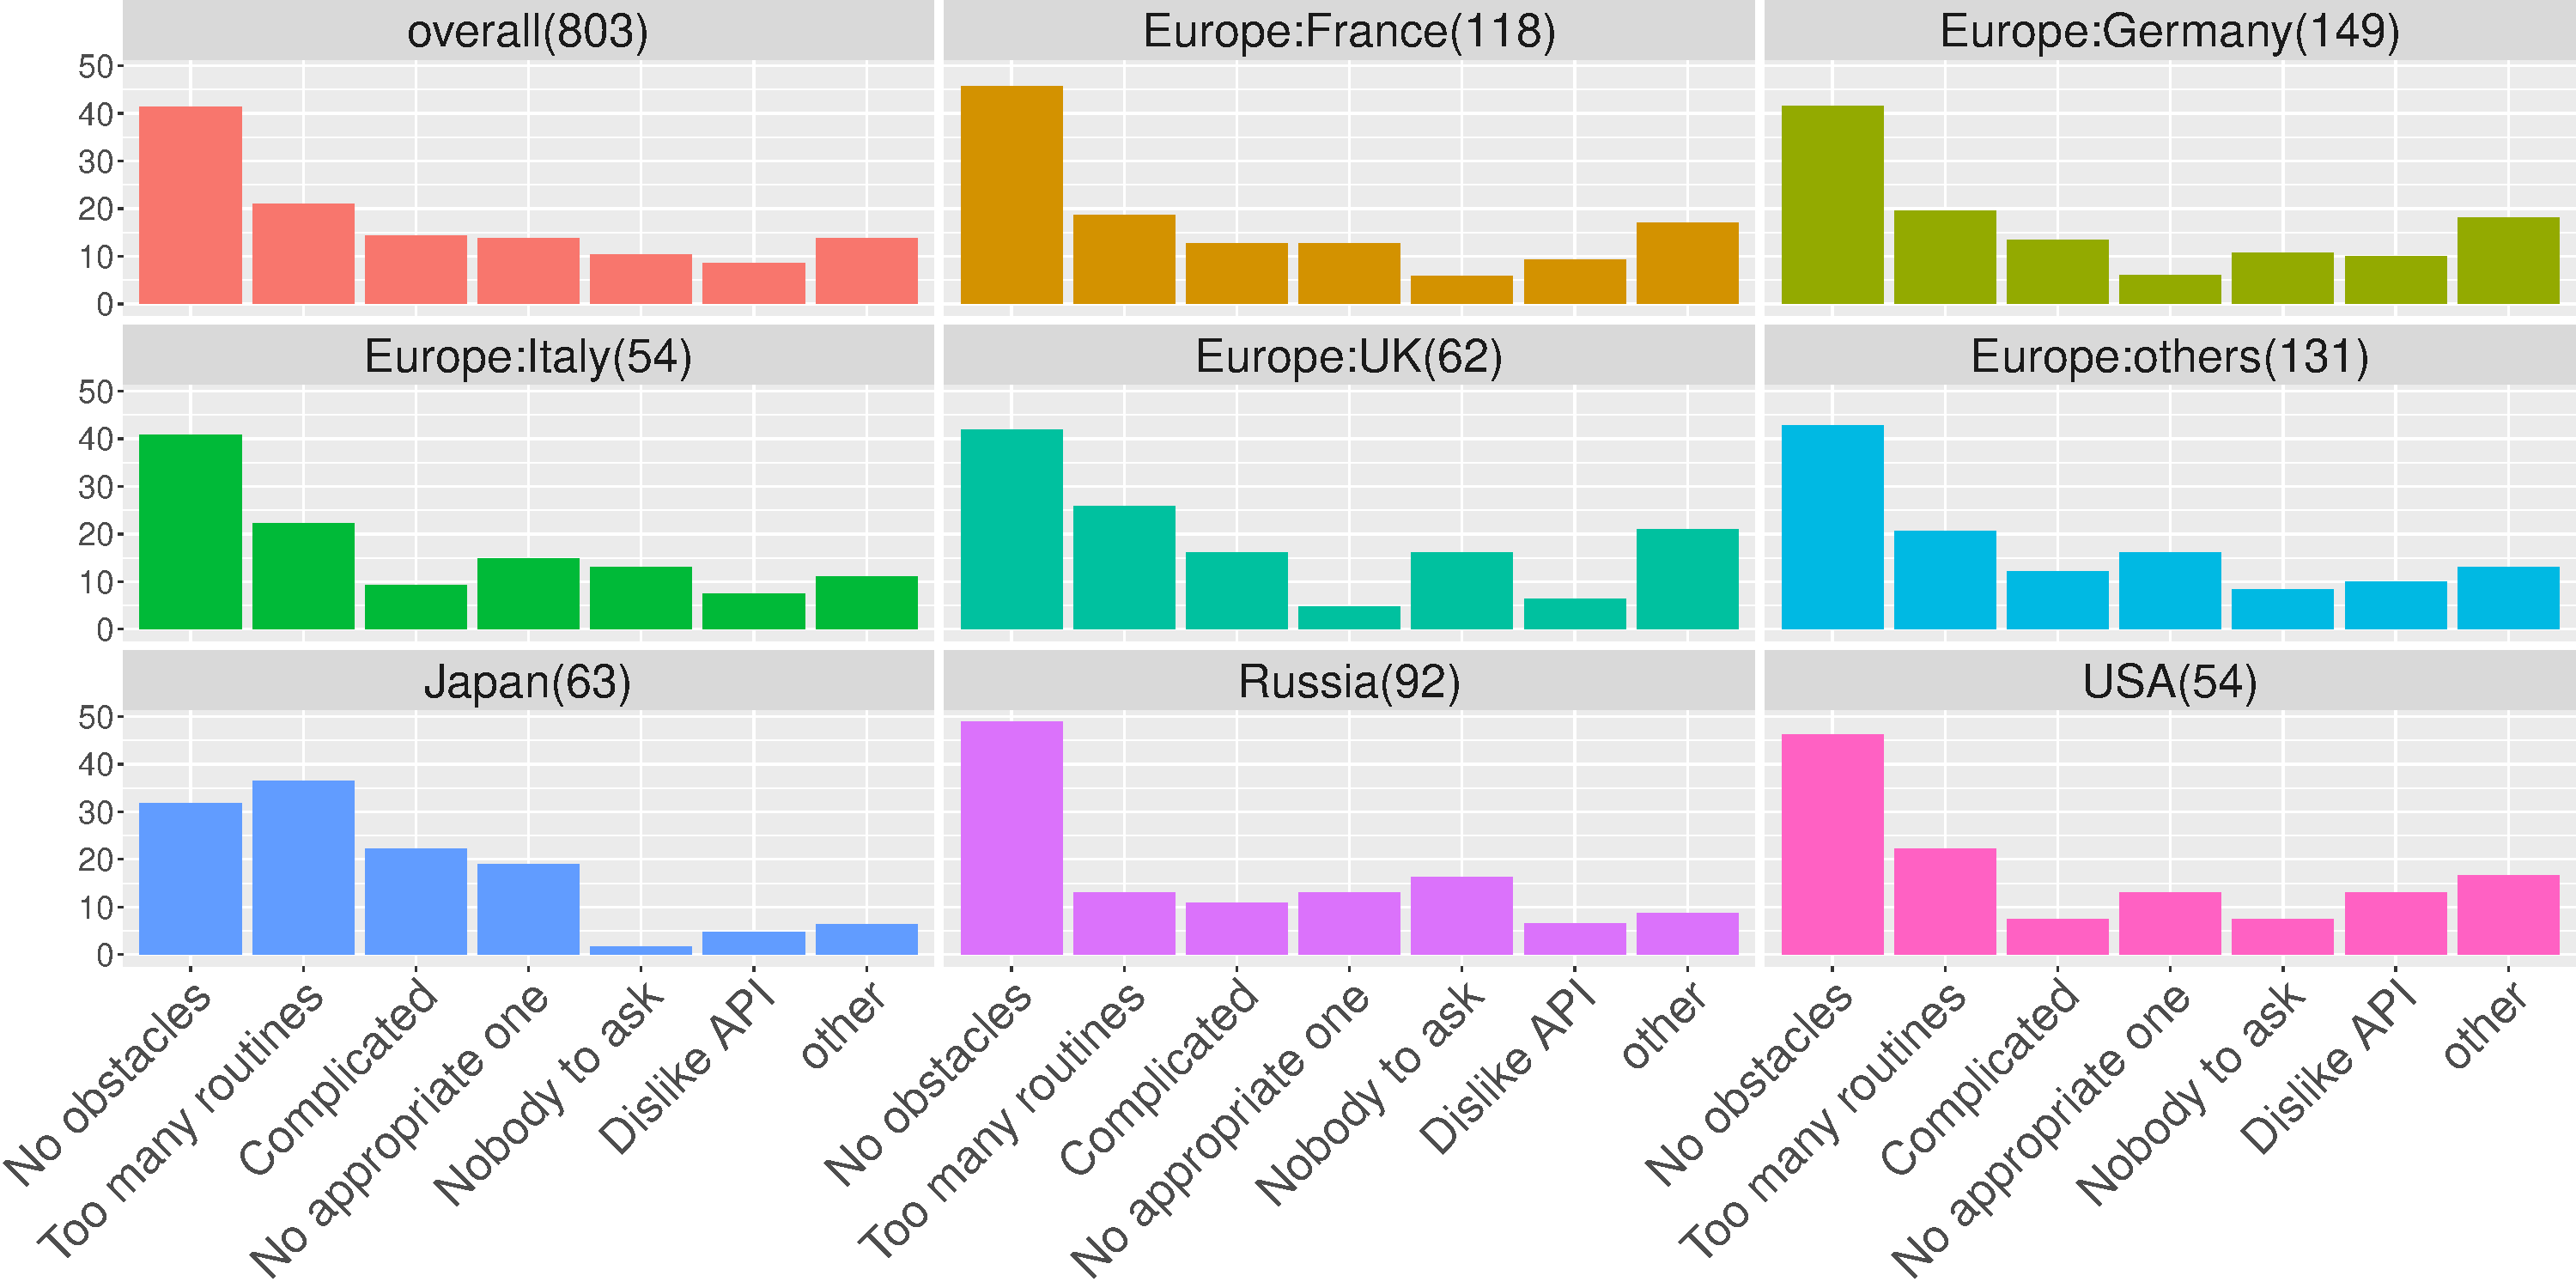
\includegraphics[width=8.7cm]{R-scripts/Q19.pdf}
\caption{Q19: Learning Obstacles {\it(multiple)}}
\label{fig:learning-obstacles}
\end{center}
\end{figure}

Generally speaking, there can be a case where a particular question in
a survey may ignite for participants to explode their dissatisfaction
by writing messages into a free text field. In our survey Q19 is
such a question. The
largest number of \myquote{other} inputs in our survey can be found
at Q19 asking \myquote{What are your obstacles to mastering MPI?}
(Fig.~\ref{fig:learning-obstacles}). Although the largest answer is
the choice of \myquote{No obstacles,} we got 111 \myquote{other} inputs
exceptionally. Q4 and Q7 are the second largest (70), but these are
because of the variety of answers.
More than 20 participants answered \myquote{other} raise
\myquote{time (to master MPI)}. Many other participants pointed
out the need of MPI programming guideline (\myquote{clear doc.},
\myquote{internal doc.}, \myquote{implementation
  doc.}, \myquote{performance guideline}, and so on, in their words).
Some participants complaints about MPI implementations and the
(performance or specification) differences among implementations.

\begin{figure}[htb]
\begin{center}
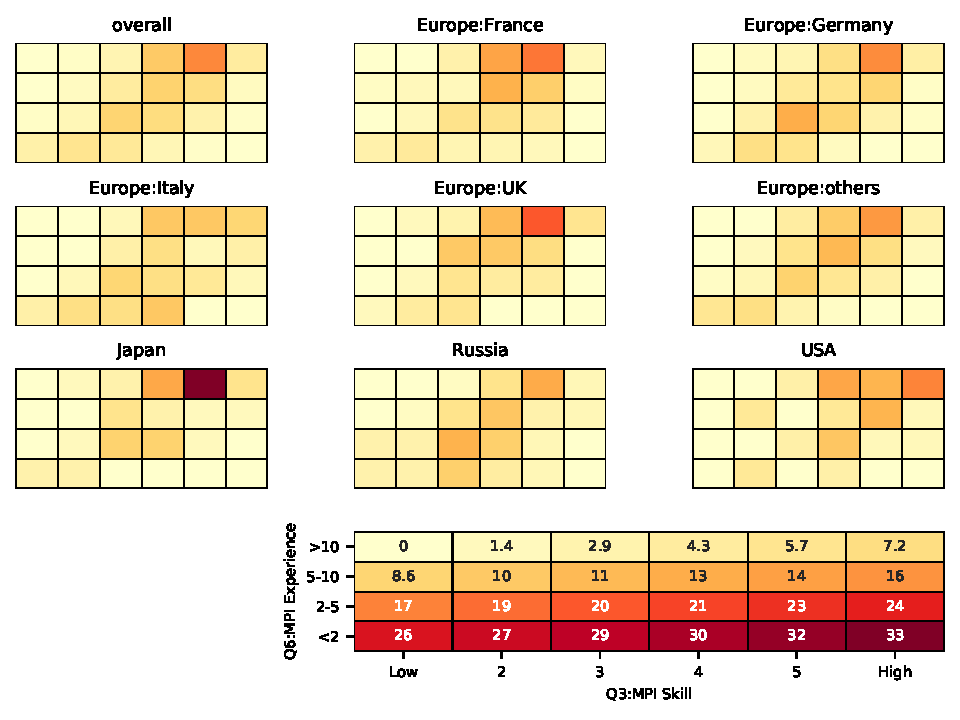
\includegraphics[width=8.7cm]{Figs/Q6-Q3.pdf}
\caption{Q6-Q3: MPI Experience {\it(single)} and MPI Skill {\it single}}
\label{fig:experience-and-skill}
\end{center}
\end{figure}

As shown in Fig.~\ref{fig:experience-and-skill}, the cross-tab heatmap
graphs between Q6 (Fig.~\ref{fig:mpi-experience} and Q3
(Fig.~\ref{fig:mpi-skill}), there is a strong correlation, from
lower-left to higher-right, between those
two questions regardless to countries or regions. And these graphs
tell that it takes more than 10 years of MPI programming experience to
reach the high MPI skill (\myquote{4} to \myquote{High}) in most
countries and regions. Many MPI users in US can reach the high
(\myquote{4} or higher) MPI skill in 5 to 10 years. Hence, it takes
more than 5 or 10 years to reach the high MPI skill
mostly. Considering this fact
and the profound nature of MPI specification
(Subsection~\ref{sec:mpi-aspects}), MPI could be said to be very
difficult library to master.

\subsection{MPI Programming Difficulty and Tuning}

Fig.~\ref{fig:difficulty} shows the result of Q15 asking \myquote{What is the
most difficult part of writing an MPI program?} and
Fig~\ref{fig:tuning} shows the result of Q23 asking \myquote{Is there any
room for performance tuning in your MPI programs?} The largest part
of US and UK participants chose \myquote{algorithm design} whilst the
participants of the other countries and regions chose
\myquote{Debugging}. In US, the second largest choice was
\myquote{Domain Decomposition}. In Japan, the second largest is
\myquote{Tuning}.

\begin{figure}[htb]
\begin{center}
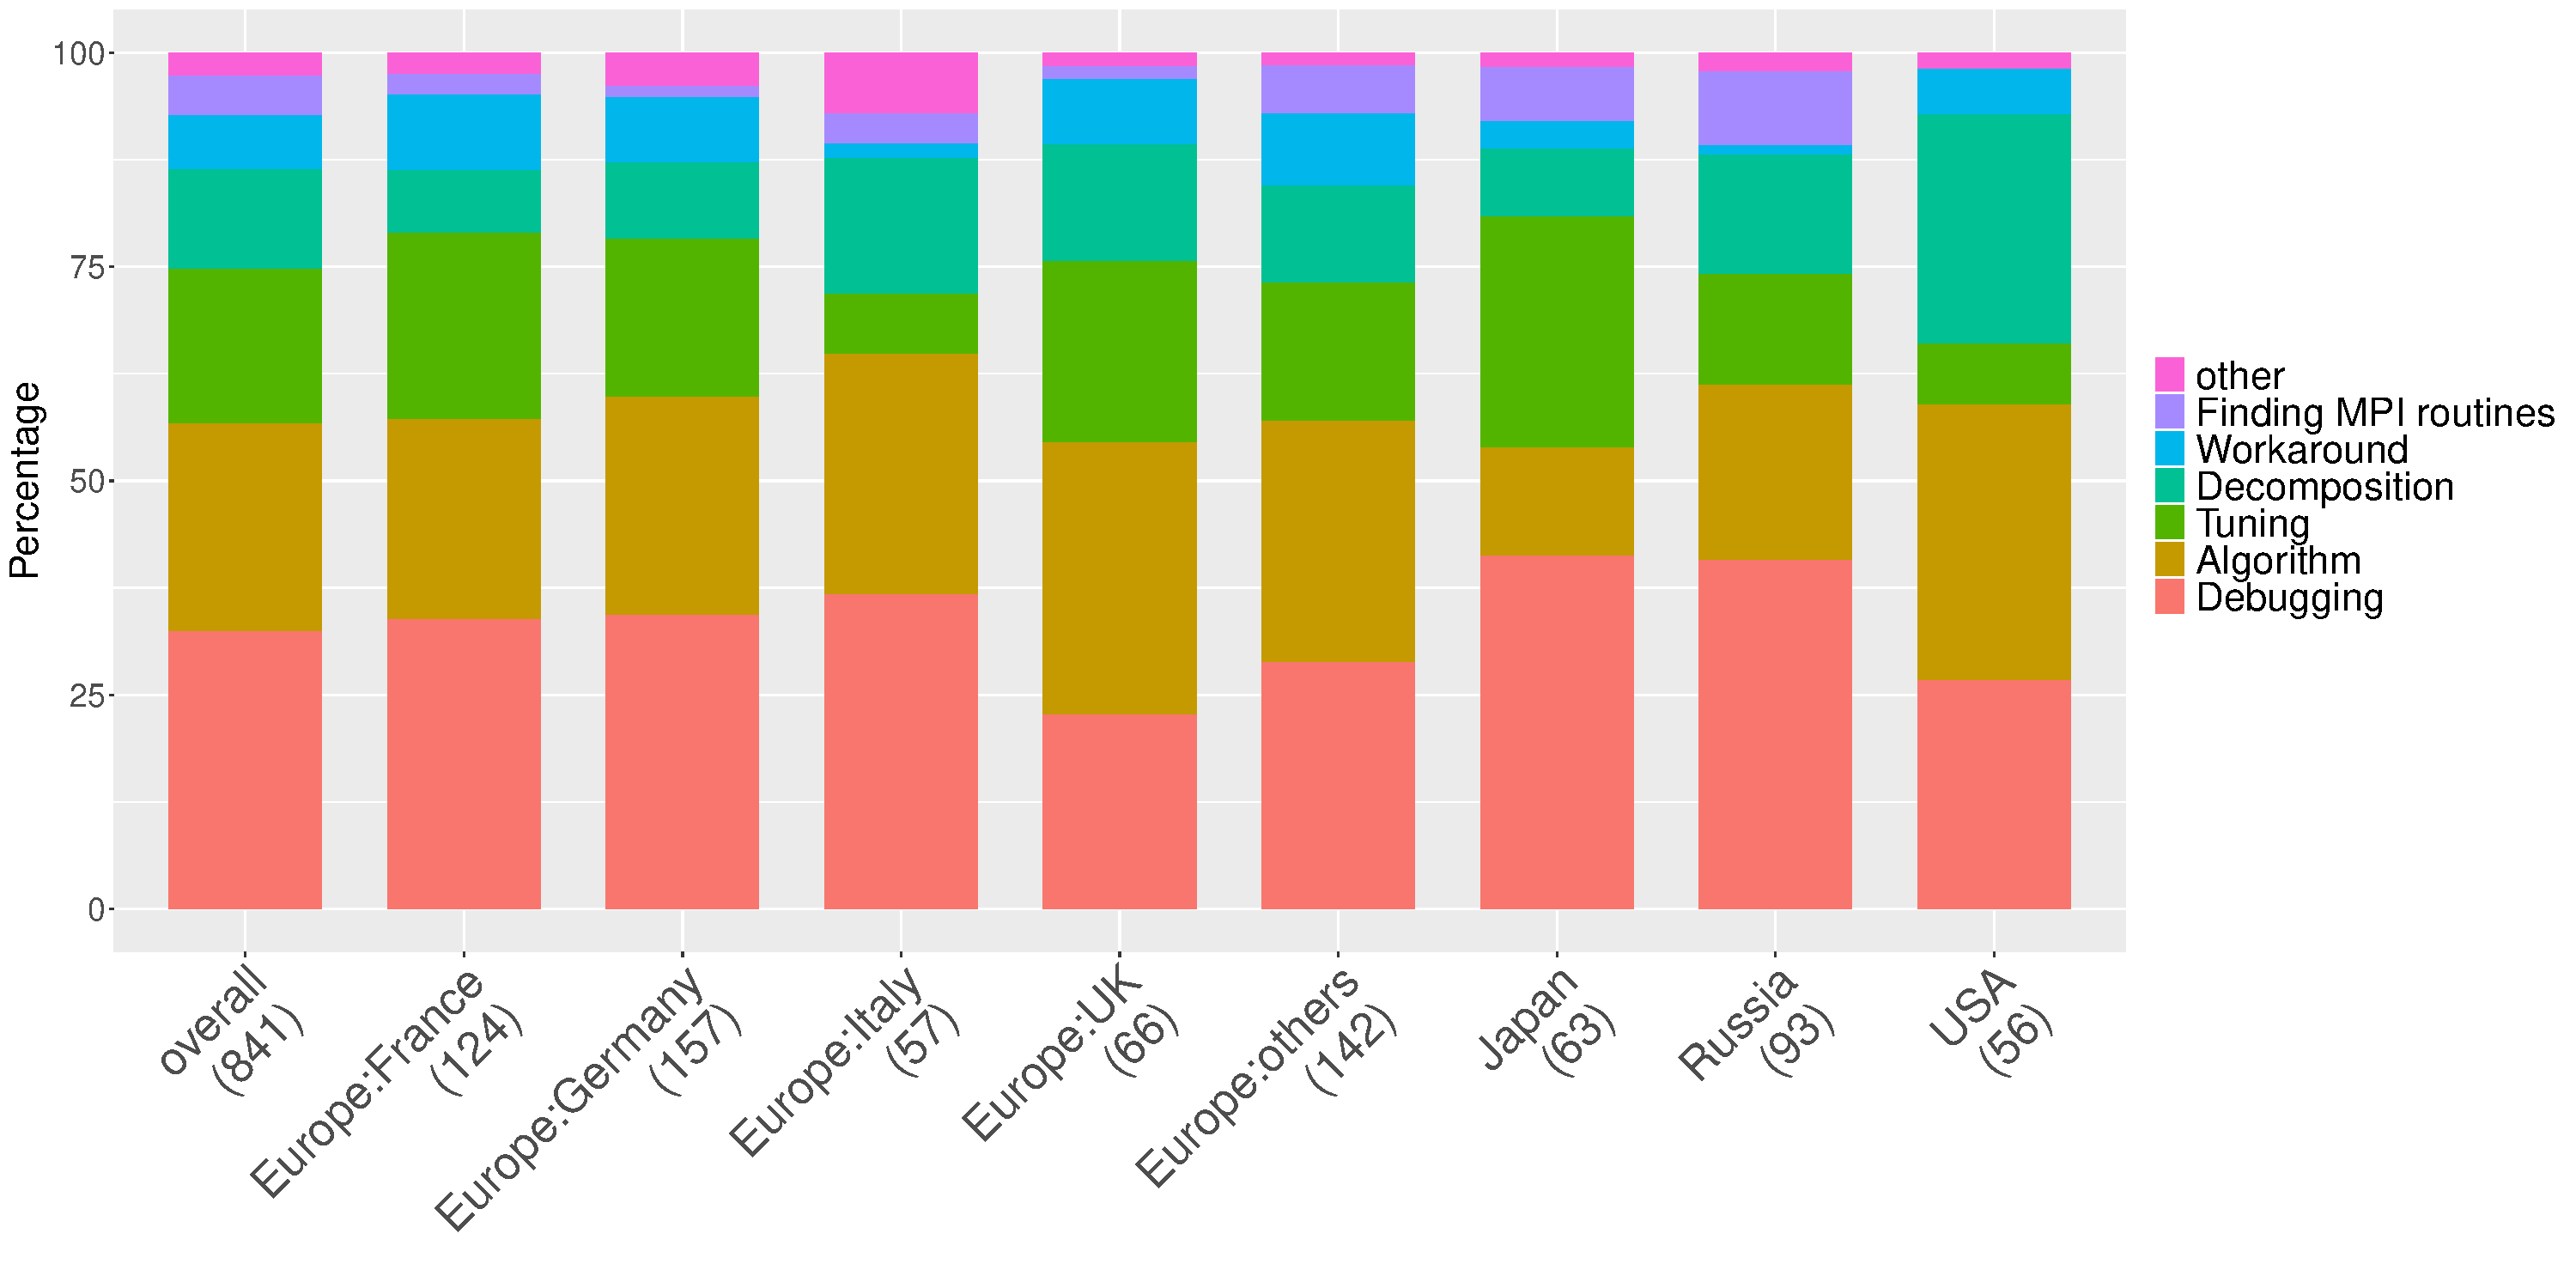
\includegraphics[width=8.7cm]{R-scripts/Q15.pdf}
\caption{Q15: MPI Programming Difficulty {\it(single)}}
\label{fig:difficulty}
\end{center}
\end{figure}

Fig.~\ref{fig:tuning} has more divergence than
Fig~\ref{fig:difficulty}. The participants selected \myquote{my MPI
  programs are well-tuned} is only around 10\% excepting Japan and
Russia. There seems to be a lots of room to tune MPI programs in
general, however, around 40\% of participants said they do not have
enough resource to do that. In Japan, the percentage of well-tuned
program is only few percent. Contrastingly, Russian percentage of
choosing \myquote{well-tuned} is the highest among the countries and
regions.

\begin{figure}[htb]
\begin{center}
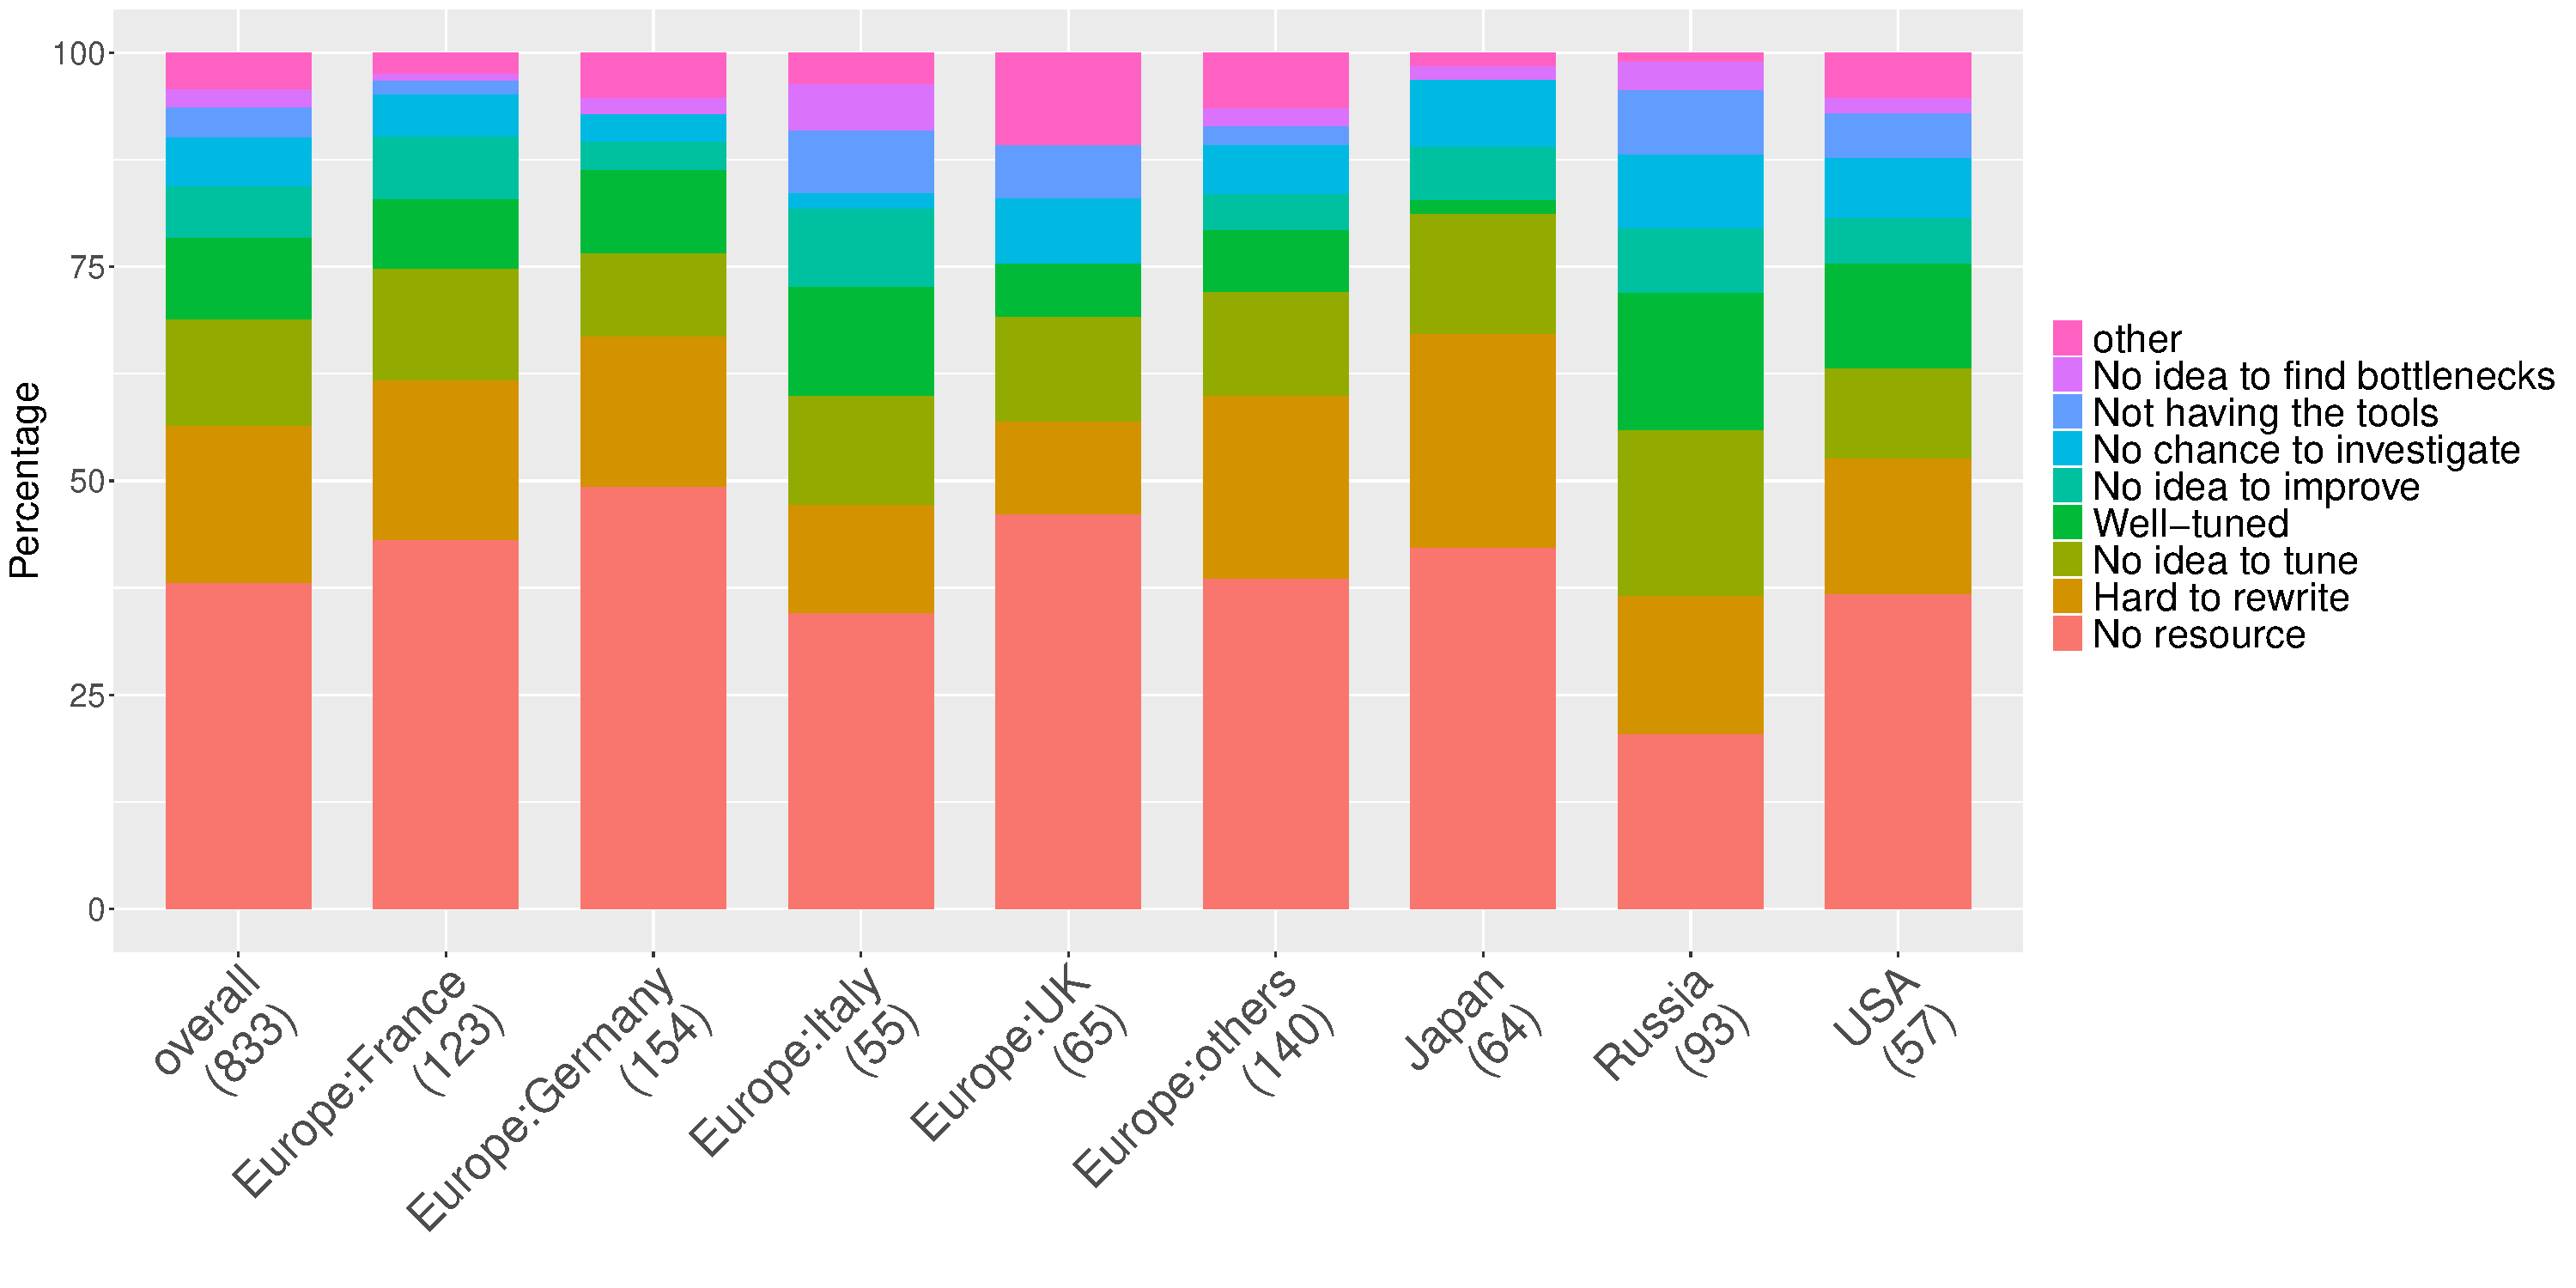
\includegraphics[width=8.7cm]{R-scripts/Q23.pdf}
\caption{Q23: Performance Tuning {\it(single)}}
\label{fig:tuning}
\end{center}
\end{figure}

\subsection{Missing Features and Semantics}

It is a general concern how MPI provides optimization
opportunities in terms of hardware capabilities such as being able to
handle the various topologies of hardware components more
efficiently. To answer this, Q25 asking \myquote{If there were one
communication aspect which is not enough in the current MPI could
improve the performance of your application, what would you
prioritize? Or $\ldots$} (Fig.~\ref{fig:missing-features}), and Q26 asking
\myquote{Is MPI providing all the communication semantics required by your
application? If not, what is missing?}
(Fig.~\ref{fig:missing-semantics}) were prepared.

In Fig.~\ref{fig:missing-features}, only 23\% of overall MPI users
are satisfied with the current situation.
Interestingly enough the second largest percentage is
\myquote{additional comm. opt.} (\myquote{Additional optimization
  opportunities in terms of communication (network topology awareness,
  etc.)}, followed by \myquote{Multi-thread} and \myquote{Other
  opt.} (\myquote{Optimization opportunities except communication
  (architecture awareness, dynamic processing, accelerator support,
  etc.)}).

\begin{figure}[htb]
\begin{center}
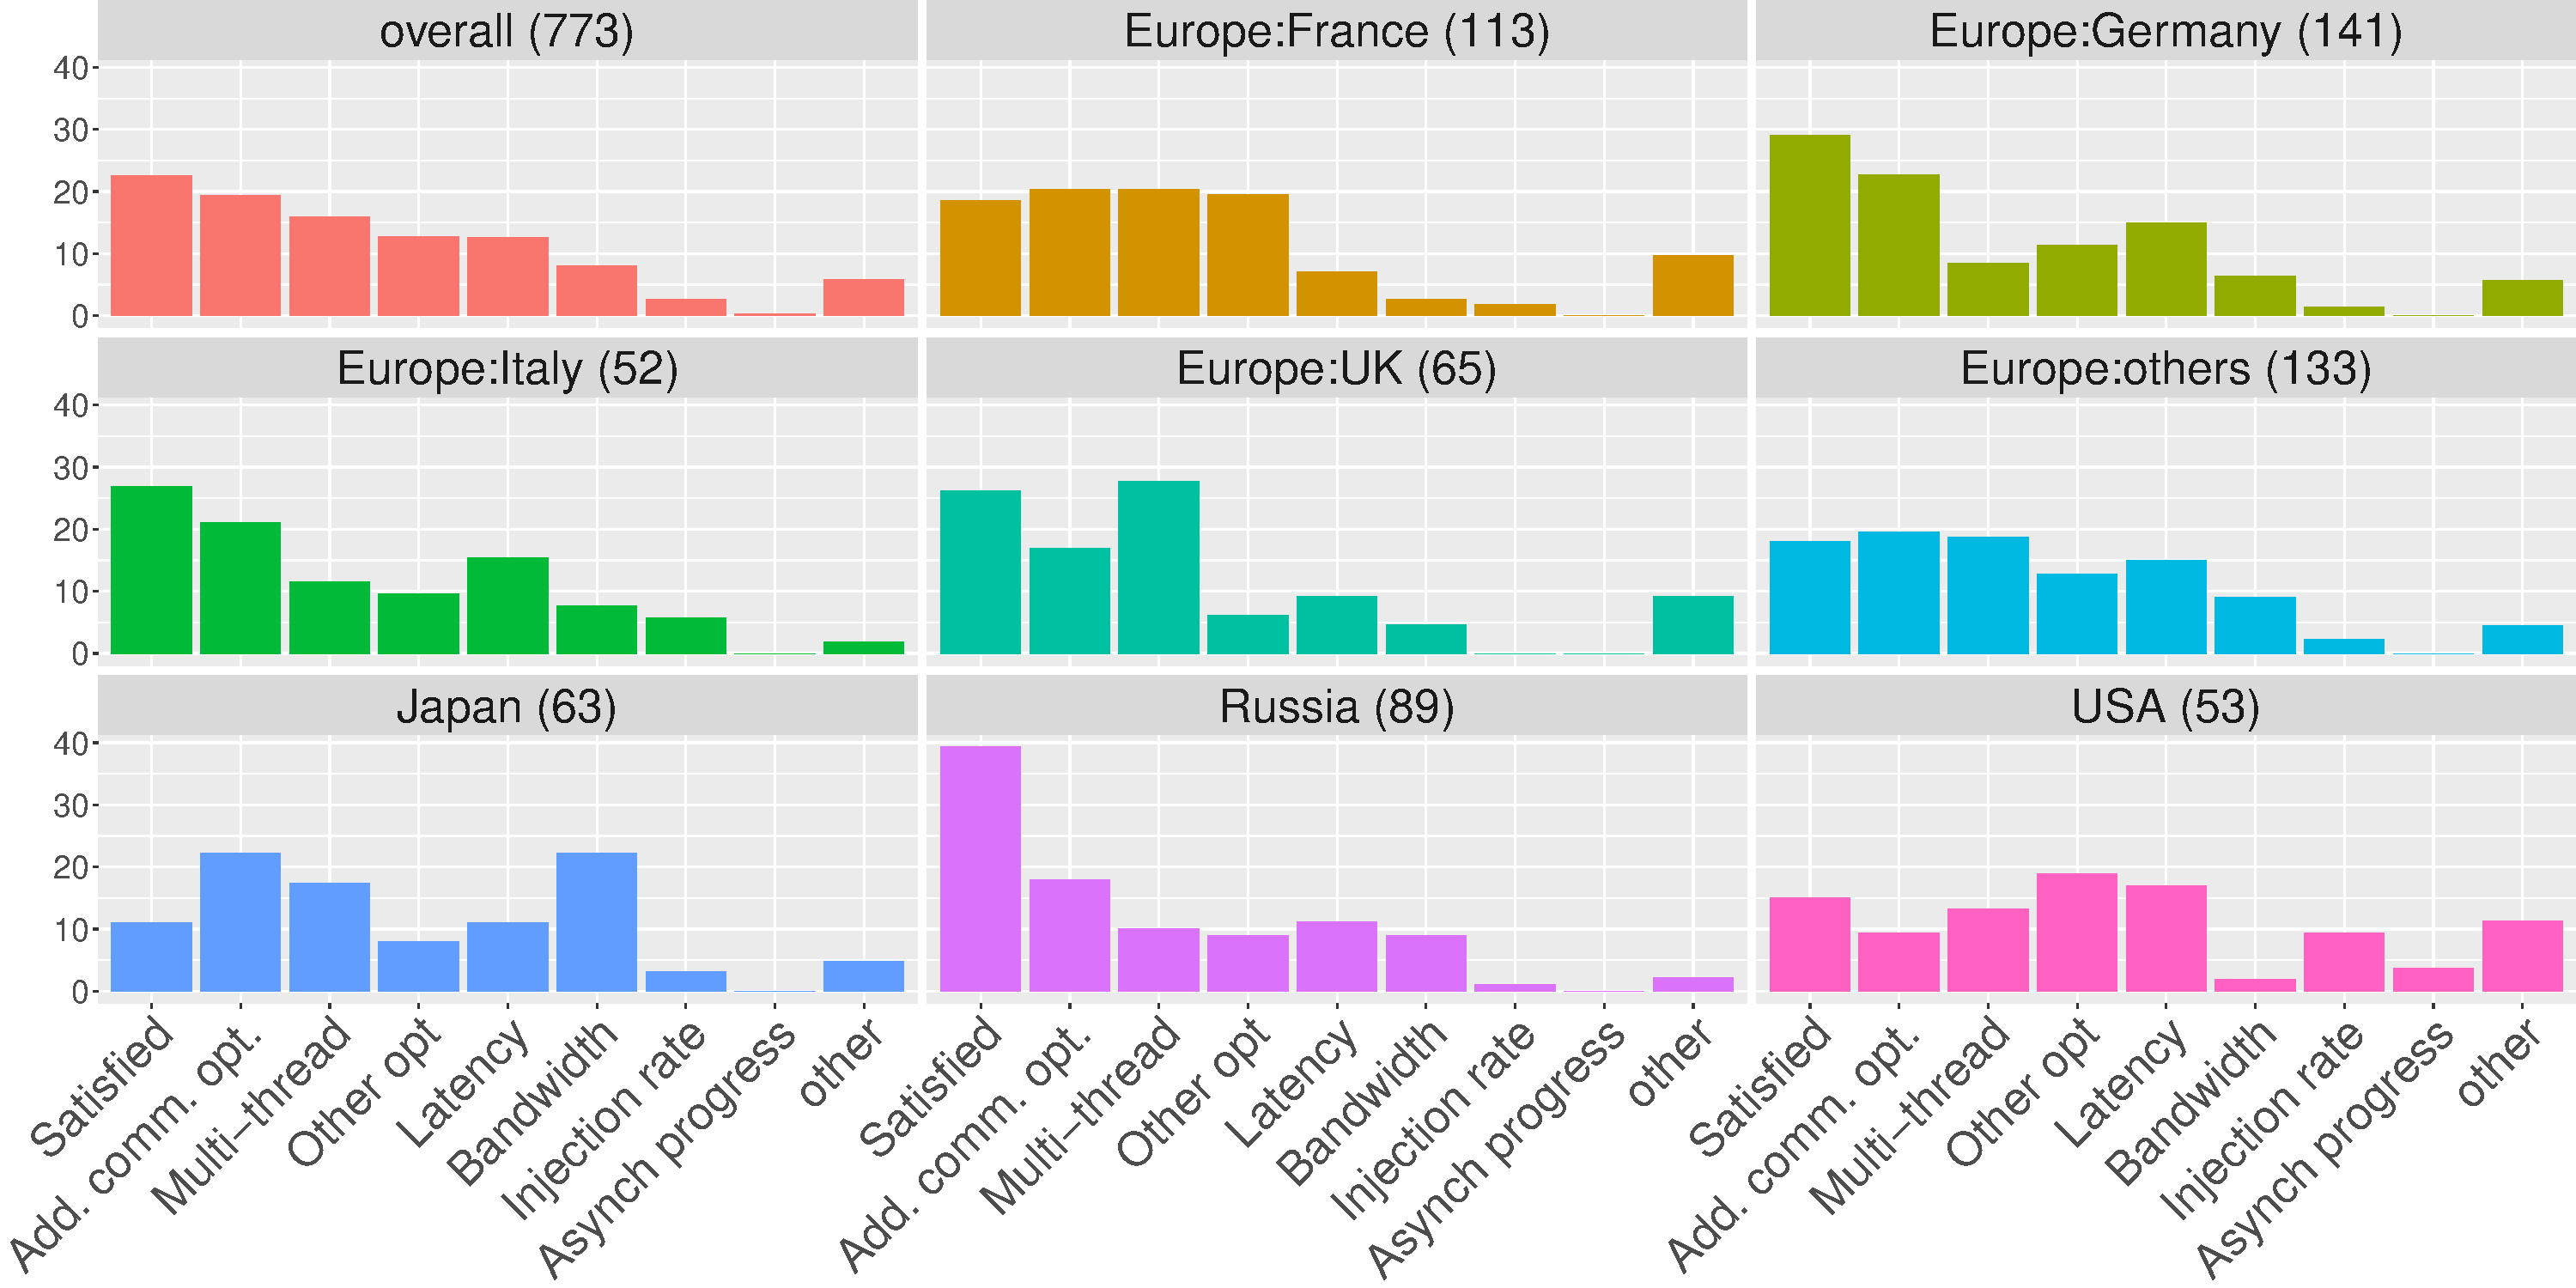
\includegraphics[width=8.7cm]{R-scripts/Q25.pdf}
\caption{Q25: Features to improve {\it(single)}}
\label{fig:missing-features}
\end{center}
\end{figure}

Q26 is somewhat similar to Q25, but looking for more precise answers.
This question tackles the issue on which semantic feature is missing
from MPI. Overall a very similar picture emerges with Q25, almost one
third of the participants are satisfied with the current
situation. There is a high discrepancy between Japan where users are
the least satisfied with the current situation and Russia which is
the most satisfied. The same situation can be seen in Q25. The highest
given answer concerns \myquote{Add. opt} (\myquote{Additional
  optimization opportunities in terms of communication (topology
  awareness, locality, etc.)}). This is coherent with Q25 and managing
efficiently the topology and the locality seem a major concern to many
users. Then
comes the concerns about the lack of resilience, a concern shared by
more than 20\% of the participants. It is very interesting that most
countries concern about the resilience. Hiding latency through
generalization of asynchrony over the whole set of functions is
another point raised repeatedly. 16\% of the users think that a
simpler and easier API would be desirable.
Although there are relatively big disparity in the satisfaction
(answering \myquote{MPI provides all}), the disparities of the other
answers are smaller.

\begin{figure}[htb]
\begin{center}
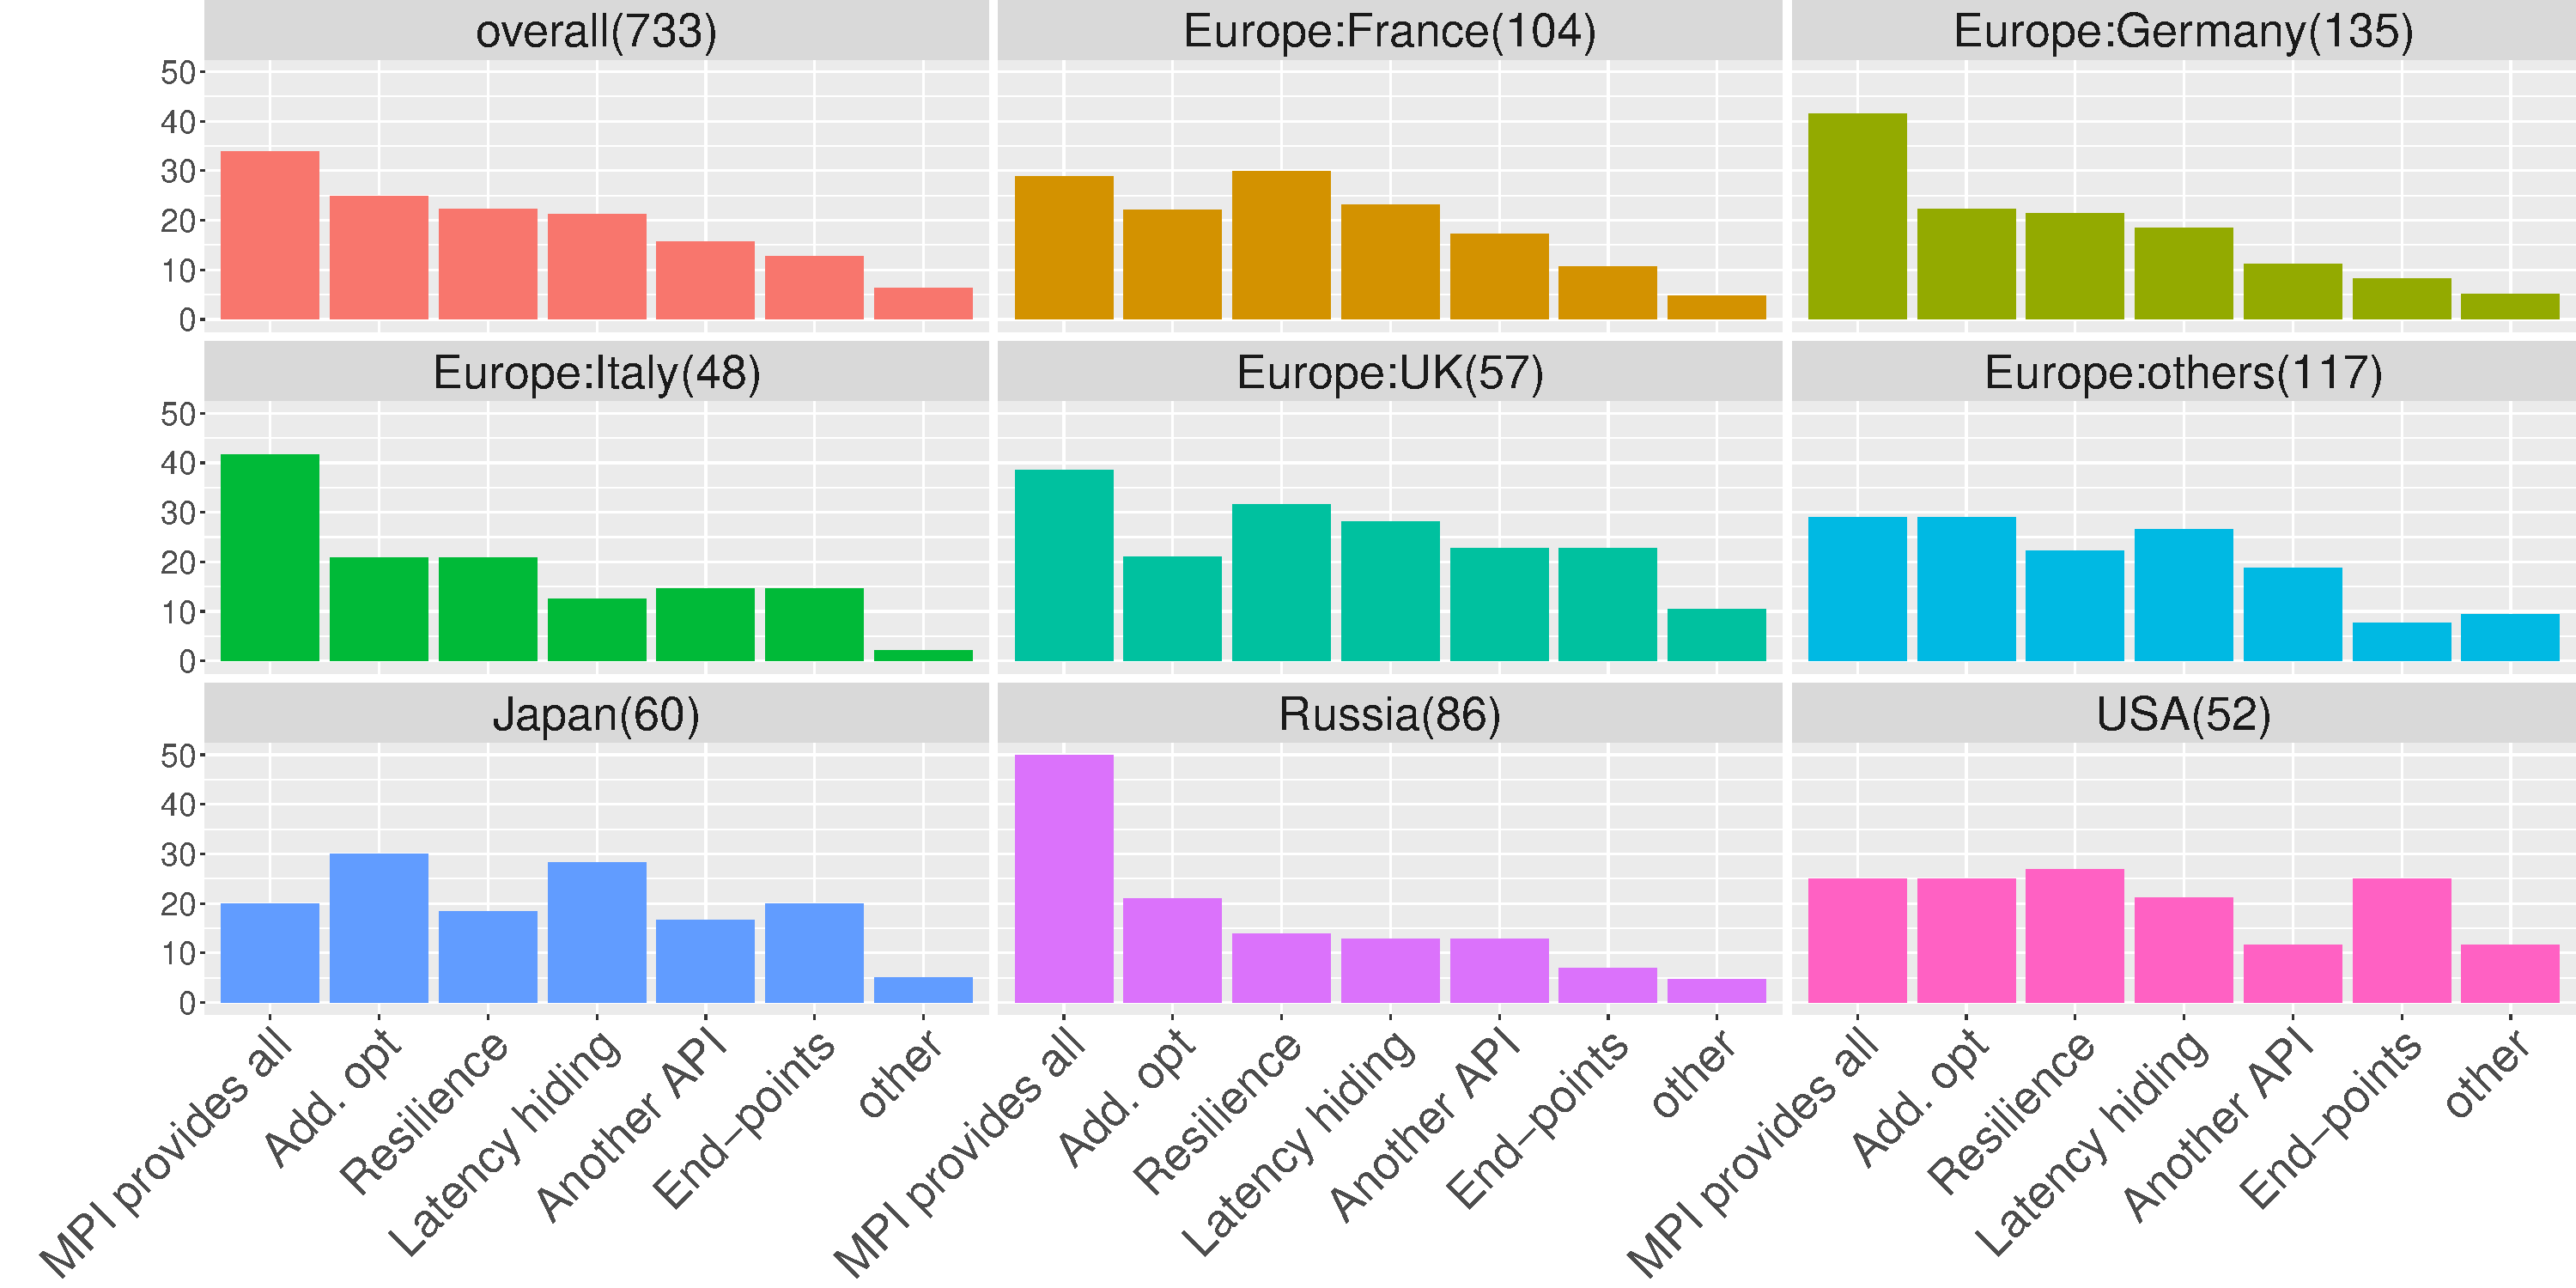
\includegraphics[width=8.7cm]{R-scripts/Q26.pdf}
\caption{Q26: MPI Missing Semantics {\it(multiple)}}
\label{fig:missing-semantics}
\end{center}
\end{figure}

Finally, the least desired feature concerns the notion of endpoints,
as discussed in the MPI standardization effort. However taking into
account the extremely
technical aspect of this question, and it's intricate evolution in the
standard, it might be possible that most people answering this
question knew little, and possible imprecisely, what this feature was
exactly about.

\subsection{Notes on Countries and Regions}

In this Subsection, we summarize our findings on some countries
showing somewhat different results with the others.

\subsubsection*{USA}

US has the highest percentages;
\begin{enumerate*}
\item having the high MPI skill (Fig.~\ref{fig:mpi-skill}),
\item using MPI more than 10 years (Fig.~\ref{fig:mpi-experience}),
\item using the {\tt MULTIPLE} threading support
  (Fig.~\ref{fig:multi-thread}),
\item choosing familiar MPI implementations
  (Fig.~\ref{fig:choosing-implementation}), and
\item reading MPI books (Fig.~\ref{fig:learning-mpi})
\end{enumerate*}
among the countries/regions. All these results indicates that the MPI
users in US are most advanced.

\subsubsection*{Russia}

Russia is;
\begin{enumerate*}
\item having the second largest percentage of MPI users less than 5
  years of MPI experience, as well as Italy
  (Fig.~\ref{fig:mpi-experience}),
\item having the largest percentage of (non-MPI) programming beginners
  (Fig:\ref{fig:prog-skill}),
\item having the highest percentage of thinking their MPI programs are
  well-tuned (Fig.~\ref{fig:difficulty}),
\item having the highest percentage not knowing which thread level
  they are using (Fig.~\ref{fig:multi-thread}), and
\item the second highest country, next to US, choosing the MPI+CUDA
  (Fig.~\ref{fig:mpi-x}).
\end{enumerate*}

These findings may indicate that Russia is relatively younger in terms
of MPI usage than the other countries/regions. The high concern on
MPI+CUDA, however, is very interesting.

\subsubsection*{Japan}

In this survey, Japan shows the most unique results (this is already
reported in~\cite{swopp2019}). Despite the high MPI
skill (Fig.~\ref{fig:mpi-skill}) and long MPI experience
(Fig.~\ref{fig:mpi-experience}), many Japanese MPI users seem to be
suffered from debugging and tuning (Fig.~\ref{fig:difficulty}), whilst
many participants of the other countries raise \myquote{Algorithm}.

Most notably, more than 50\% of Japanese MPI users have the MPI
experience more than 10 years exceptionally. This would sound good,
however, the equally distributed answers is desired, thinking the
continuous alternation of generations. The percentage of 5-to-10-year
MPI experience in Japan is the smallest among the countries. If this
lack of mid-level is true, then the future of Japanese HPC community
would not be bright.

\section{Discussion}

\subsection{Inflating standard}

As this survey reveals that some MPI features, which were already
introduced almost a decade ago, are not widely accepted by MPI users
yet (Subsection \ref{sec:mpi-aspects}). Here a question may be raised,
if this gap between the MPI features defined by the standard and the
acceptance of the features will become wider or narrower?

\begin{figure}[htb]
\begin{center}
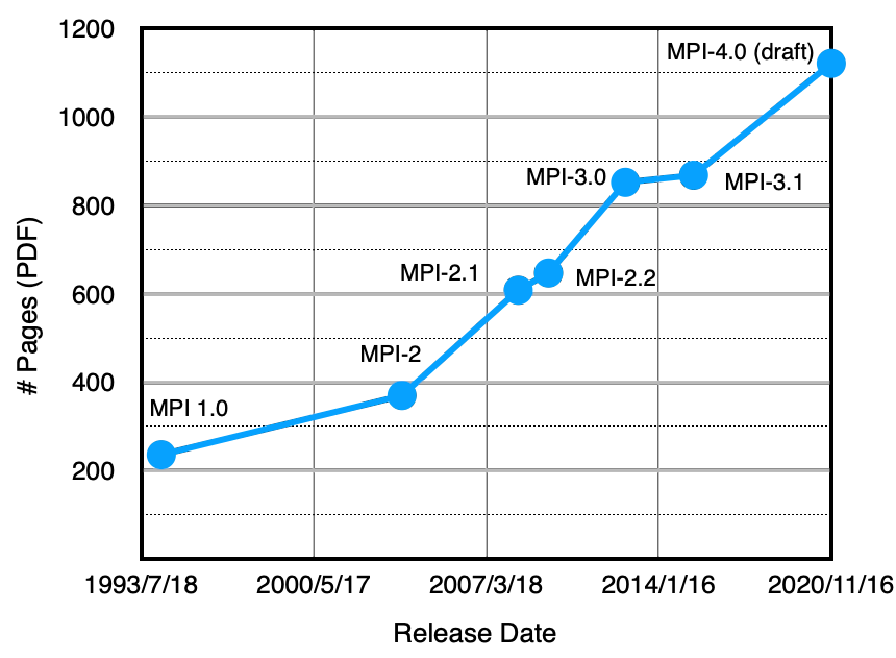
\includegraphics[width=8cm]{Figs/MPI-Standards.pdf}
\caption{Page sizes of MPI Standards}
\label{fig:mpi-standards}
\end{center}
\end{figure}

Fig.~\ref{fig:mpi-standards} shows the number of pages (in terms of
PDF, not the content) plotted over the released dates. Not
surprisingly, the number of pages increases every time newer standard
is released. It is a natural thinking that the number of pages and the
number of features are proportional.

In many cases, the higher functionalities introduced by newer MPI
standard yield more degree of implementation freedom. An MPI
implementation can optimized its performance by exploiting hardware
resources without having the MPI users large effort. If only the most
basic communication functions, send and receive, are supported by MPI
then users have to write collective functions which are not easy if
users wants optimize for the parallel machines they are using.

Another reason of the inflation is that MPI standard is the standard
as a library. There is no way for library functions to know how the
library functions are called in which context. The higher abstracted
functions can give a library more information of how and which and
thus the higher-level functions can be optimized. Traf, et al., gives
a formal analysis on this point\cite{5184825}.
This situation, introducing higher-level functions into the standard,
inflates the standard and always will be. And the gap will not be
narrowed.

Hoefler et al., reported their idea to extract collective operation
patterns from a series of communication primitives, send and
receive\cite{7842939}, at run time. Applying this technique, a
communication library will be able to optimize various communication
patterns without introducing higher-level functions.
Although their idea is at the experimental
stage, however, this seems to be a good solution not introducing new
functions but narrowing the gap.

\subsection{Recommendation as a result of this survey}

Currently the MPI standard documents are available in PDF format and
hardcover books~\cite{mpi-hardcover}. There are some MPI tutorial web
sites (\cite{mpi-tutorial} as an example). \cite{mpi-tutorial-intro}
pointed out most of such web pages are out-dated and not
thorough.

As already shown in Subsection~\ref{sec:mpi-aspects}, some MPI
features, which are not newly introduced, have failed to be
well-known. Further many MPI users have not enough time to master MPI
as described in Subsection~\ref{sec:learning-mpi}. These suggest that
there is something wrong for people to learn MPI and writing MPI
programs.

Thus, it is very important to narrow the gap described in the previous
subsection by helping MPI users to learn and write MPI programs. We
believe this is the responsibility of MPI Forum, since the other,
volunteer-based approach would not be efficient and sufficient. If
MPI Forum agrees with us for narrowing the gap, then MPI Forum should

\begin{itemize}
\item {\bf slow the pace of introducing new features,} and
\item {\bf create a new working group to prepare and maintain web pages for
  tutorial, guidelines for MPI programming, and good (and bad) MPI
  examples}.
\end{itemize}

\section{Summary}

We have conducted a questionnaire survey and succeeded to gather more
than 850 participants from more than 40 countries and regions. By
analyzing the collected data, we could get several findings. As for
the MPI features, the dynamic process feature is considered not only
as a less-used feature but also a useless feature (highlighting that
the MPI programming model is seen as {\em static}). By asking several
questions how participants obtain MPI knowledge and experiences, it is
revealed that MPI is a very difficult-to-use library.
Most participants read the MPI standard only partially to check the
specification of MPI functions. Instead many MPI users desire to have
practical programming guideline, online documents in
hyper-text form, and useful sample programs. Most important
(and most difficult) thing is those supplemental
documents in any form must be up-to-dated and thorough. For the
compatibility, many MPI users may accept to sacrifice the
compatibility to get more performance.

All collected answers, the programs to analyze the survey data and to
generate graphs, and all published reports are available at
{\tt \url{https://github.com/bosilca/MPIsurvey.git}}.

\section*{Acknowledgments}

We thank to those who participated in this survey and those who
helped us to distribute the questionnaire to their local
communities. We especially thank to MPI Forum members who gave us many
significant comments on the draft questionnaire.
This research is partially supported by the
NCSA-Inria-ANL-BSC-JSC-Riken-UTK Joint-Laboratory for Extreme Scale
Computing~\cite{JLESC}.

\bibliography{ref}

{\footnotesize
  \begin{description}
  \item[{[dataset][19]}] A. Hori, T. Ogura, E. Jeannot,
G. Bosilca, MPI International Survey – GitHub Repository,
\url{https://github.com/bosilca/MPIsurvey.git}, 2021.
  \end{description}
}

\appendix
\section{List of Questions and Choices}
\label{app:questions}

The followings are the list of all questions associated with
choices. The question numbers suffixed by asterisks (*) are
multiple-answer questions. The choices are followed by corresponding
abbreviations in square brackets, if any.
\vspace{3mm}
{\small
  \begin{description}
  \item[Q1:] What is your main occupation
    \begin{inparaenum}[{\bf C}1)]
    \item College/University [Univ]
    \item Governmental institute [Gov]
    \item Hardware vendor [HW]
    \item Software vendor [SW]
    \item Private research institute [priv]
    \item Other
    \end{inparaenum}
  \item[Country:] \hspace{3mm}Select main country or region of your workplace in past 5 years.
    Choose one from the country list.
  \item[Q2:] Rate your overall programming skill (non-MPI programs).
    Choose one in the range of 1 to 6. [Low-High]
  \item[Q3:] Rate your MPI programming skill.
    Choose one in the range of 1 to 6. [Low-High]
  \item[Q4*:] What programming language(s) do you use most often?
    \begin{inparaenum}[{\bf C}1)]
    \item C/C++ [C(++)]
    \item Fortran 90 or newer [\textgreater=F90]
    \item Fortran (older one than Fortran 90) [\textless F90]
    \item Python [Py]
    \item Java [Java]
    \item Other
    \end{inparaenum}
  \item[Q5:] How long have you been writing computer programs (incl. non-MPI programs)?
    \begin{inparaenum}[{\bf C}1)]
    \item more than 10 years [\textgreater10]
    \item between 5 and 10 years [5-10]
    \item between 2 and 5 years [2-5]
    \item less than 2 years [\textless 2]
    \end{inparaenum}
  \item[Q6:] How long have you been writing MPI programs?
    \begin{inparaenum}[{\bf C}1)]
    \item more than 10 years [\textgreater10]
    \item between 5 and 10 years [5-10]
    \item between 2 and 5 years [2-5]
    \item less than 2 years [\textless 2]
    \end{inparaenum}
  \item[Q7*:] Which fields are you mostly working in?
    \begin{inparaenum}[{\bf C}1)]
    \item System software development (OS, runtime library, communication
      library, etc.) [OS/R]
    \item Parallel language (incl. domain specific language) [Lang]
    \item Numerical application and/or library [Num-App/Lib]
    \item AI (Deep Learning) [AI]
    \item Image processing [Image Proc]
    \item Big data [Bg Data]
    \item Workflow and/or In-situ [Workfflow]
    \item Visualization [Visualization]
    \item Tool development (performance tuning, debugging, etc.) [Tool]
    \item Other
    \end{inparaenum}
  \item[Q8*:] What is your major role at your place of work?
    \begin{inparaenum}[{\bf C}1)]
    \item Research and development of application(s) [Apps]
    \item Research and development software tool(s) [Tools]
    \item Parallelization of sequential program(s) [parallelize]
    \item Performance tuning of MPI program(s) [Tuning]
    \item Debugging MPI programs [Debug]
    \item Research and development on system software (OS and/or runtime
      library) [OS/R]
    \item Other
    \end{inparaenum}
  \item[Q9:] Have you ever read the MPI standard specification document?
    \begin{inparaenum}[{\bf C}1)]
    \item I read all. [All]
    \item I read most of it. [Mostly]
    \item I read only the chapters of interest for my work. [Partly]
    \item I have not read it, but I plan to. [Wish]
    \item No, and I will not read it. [No]
    \end{inparaenum}
  \item[Q10*:] How did you learn MPI?
    \begin{inparaenum}[{\bf C}1)]
    \item I read the MPI standard document. [Standard]
    \item I had lecture(s) at school. [School]
    \item I read articles found on Internet. [Internet]
    \item I read book(s). [Books]
    \item Other lectures or tutorials (workplace, conference). [Other lec.]
    \item I have not learned MPI. [Never learned]
    \item Other
    \end{inparaenum}
  \item[Q11*:] Which MPI book(s) have you read?
    \begin{inparaenum}[{\bf C}1)]
    \item Beginning MPI (An Introduction in C) [Beginning MPI]
    \item Parallel Programming with MPI [Parallel Programming]
    \item Using MPI [Using MPI]
    \item Parallel Programming in C with MPI and OpenMP [Parallel
      Programming in C]
    \item MPI: The Complete Reference [MPI: Complete Ref]
    \item I have never read any MPI books [(no book)]
    \item Other
    \end{inparaenum}
  \item[Q12*:] Which MPI implementations do you use?
    \begin{inparaenum}[{\bf C}1)]
    \item MPICH
    \item Open MPI [OMPI]
    \item Intel MPI [Intel]
    \item MVAPICH [MVA]
    \item Cray MPI [Cray]
    \item IBM MPI (BG/Q, PE, Spectrum) [IBM]
    \item HPE MPI [HPE]
    \item Tianhe MPI [Tianhe]
    \item Sunway MPI [Sunway]
    \item Fujitsu MPI [Fujitsu]
    \item NEC MPI [NEC]
    \item MS MPI [MS]
    \item MPC MPI [MPC]
    \item I do not know [No idea]
    \item Other
    \end{inparaenum}
  \item[Q13:] Why did you choose the MPI implementation(s)?
    \begin{inparaenum}[{\bf C}1)]
    \item I like to use it. [I like]
    \item I was said to use it. [Said to use]
    \item I could not have any choice (the one provided by a vendor). [No choice]
    \item I am familiar with it. [Familiar]
    \item I have no special reason. [No reason]
    \end{inparaenum}
  \item[Q14*:] How do you check MPI specifications when you are writing MPI programs?
    \begin{inparaenum}[{\bf C}1)]
    \item I read the MPI Standard document (web/book). [MPI standard]
    \item I read online documents (such as man pages). [Online docs]
    \item I search the Internet (Google / Stack Overflow). [Internet]
    \item I ask colleagues. [Colleagues]
    \item I read book(s) (except the MPI standard). [Books]
    \item I know almost all MPI routines. [I know all]
    \item Other
    \end{inparaenum}
  \item[Q15:] What is the most difficult part of writing an MPI program?
    \begin{inparaenum}[{\bf C}1)]
    \item Algorithm design [Algorithm]
    \item Debugging [Debugging]
    \item Domain decomposition [Decomposition]
    \item Finding appropriate MPI routines [Finding MPI routines]
    \item Implementation issue workaround [Workaround]
    \item Performance tuning [Tuning]
    \item Other
    \end{inparaenum}
  \item[Q16*:] Which MPI features have you never heard of?
    \begin{inparaenum}[{\bf C}1)]
    \item Point-to-point communications [Point-to-point]
    \item Collective communications [Collectives]
    \item Communicator operations (split, duplicate, and so on) [Communicator]
    \item MPI datatypes [Datatypes]
    \item One-sided communications [One-sided]
    \item Dynamic process creation [Dyn. process]
    \item Persistent communication [Persistent]
    \item PMPI interface [PMPI]
    \item MPI with OpenMP (or multithread) [with OpenMP]
    \item Other
    \end{inparaenum}
  \item[Q17*:] What aspects of the MPI standard do you use in your program in its current form?
    \begin{inparaenum}[{\bf C}1)]
    \item Point-to-point communications [Point-to-point]
    \item Collective communications [Collectives]
    \item Communicator operations (split, duplicate, and so on) [Communicator]
    \item MPI datatypes [Datatypes]
    \item One-sided communications [One-sides]
    \item Dynamic process creation [Dyn. process]
    \item Persistent communications [Persistent]
    \item MPI with OpenMP (or multithread) [with OpenMP]
    \item PMPI interface [PMPI]
    \item Other
    \end{inparaenum}
  \item[Q18*:] Which MPI thread support are you using?
    \begin{inparaenum}[{\bf C}1)]
    \item MPI\_THREAD\_SINGLE [SINGLE]
    \item MPI\_THREAD\_FUNNELED [FUNNELED]
    \item MPI\_THREAD\_SERIALIZED [SERIALIZED]
    \item MPI\_THREAD\_MULTIPLE [MULTIPLE]
    \item I have never called {\tt MPI\_INIT\_THREAD} [never used]
    \item I do not know or I do not care. [Np idea]
    \item Other
    \end{inparaenum}
  \item[Q19*:] What are your obstacles to mastering MPI?
    \begin{inparaenum}[{\bf C}1)]
    \item I have no obstacles. [No obstacles]
    \item Too many routines. [Too many routines]
    \item No appropriate lecture / book / info. [No appropriate one]
    \item Too complicated and hard to understand. [Complicated]
    \item I have nobody to ask. [Nobody to ask]
    \item I do not like the API. [Dislike API]
    \item Other
    \end{inparaenum}
  \item[Q20:] When you call an MPI routine, how often do you check the error code of the MPI routine  (excepting MPI-IO)?
    \begin{inparaenum}[{\bf C}1)]
    \item I rely on the default ‘Errors abort’ error handling [Default]
    \item Always
    \item Mostly
    \item Sometimes
    \item Never
    \item Other
    \end{inparaenum}
  \item[Q21:] In most of your programs, do you pack MPI function calls into their own file or files to have your own abstraction layer for communication?
    \begin{inparaenum}[{\bf C}1)]
    \item Yes, to minimize the changes of communication API. [Yes]
    \item Yes, but I have no special reason for doing that. [Yes, but no reason]
    \item No, my program is too small to do that. [No, too small]
    \item No, MPI calls are scattered in my programs. [No, scattered]
    \item Other
    \end{inparaenum}
  \item[Q22*:] Have you ever written MPI+”X” programs?
    \begin{inparaenum}[{\bf C}1)]
    \item OpenMP [OMP]
    \item Pthread
    \item OpenACC [OACC]
    \item OpenCL [OCL]
    \item CUDA
    \item No
    \item Other
    \end{inparaenum}
  \item[Q23:] Is there any room for performance tuning in your MPI programs?
    \begin{inparaenum}[{\bf C}1)]
    \item No, my MPI programs are well-tuned. [Well-tuned]
    \item Yes, I know there is room for tuning but I should re-write large
      part of my program to do that. [Hard to rewrite]
    \item Yes, I know there is room for tuning but I do not have enough resources to do that.
      [No resource]
    \item I think there is room but I do not know how to tune it.
      [No idea to tune]
    \item I do not have (know) tools to find performance bottlenecks.
      [Not having the tools]
    \item I have no chance to investigate.
      [No chance to investigate]
    \item I do not know how to find bottlenecks.
      [No idea to find bottlenecks]
    \item I do not know if there is room for performance tuning.
      [No idea to improve]
    \item Other
    \end{inparaenum}
  \item[Q24*:] What, if any, alternatives are you investigating to
    indirectly call MPI or another communication layer by using another
    parallel language/library?
    \begin{inparaenum}[{\bf C}1)]
    \item A framework or library using MPI. [Framework]
    \item A PGAS language (UPC, Coarray Fortran, OpenSHMEM, XcalableMP,
      ...). [PGAS]
    \item A Domain Specific Language (DSL). [DSL]
    \item Low-level communication layer provided by vendor (Verbs, DCMF,
      ...). [LL comm]
    \item I am not investigating any alternatives. [No investigation]
    \item Other
    \end{inparaenum}
  \item[Q25:] If there were one communication aspect which is not enough
    in the current MPI could improve the performance of your application,
    what would you prioritize? Or is MPI providing all the communication
    semantics required by your application? If not, what is missing?
    \begin{inparaenum}[{\bf C}1)]
    \item Latency [Latency]
    \item Message injection rate [Injection rate]
    \item Bandwidth [Bandwidth]
    \item Additional optimization opportunities in terms of communication
      (network topology awareness, etc.) [Additional comm. opt.]
    \item Optimization opportunities except communication (architecture
      awareness, dynamic processing, accelerator support, etc.) [Other opt.]
    \item Multi-threading support [Multi-thread]
    \item Asynchronous progress [Asynch progress]
    \item MPI provides all semantics I need [Satisfied]
    \item Other
    \end{inparaenum}
  \item[Q26*:] Is MPI providing all the communication semantics required
    by your application? If not, what is missing?
    \begin{inparaenum}[{\bf C}1)]
    \item Latency hiding (including asynchronous completion) [Latency hiding]
    \item Endpoints (multi-thread, sessions) [End-points]
    \item Resilience (fault tolerance) [Resilience]
    \item Additional optimization opportunities in terms of communication
      (topology awareness, locality, etc.) [Additional opt]
    \item Another API which is easier and/or simpler to use [Another API]
    \item MPI is providing all the communication semantics required by my
      application [MPI provides all]
    \item Other
    \end{inparaenum}
  \item[Q27*:] What MPI feature(s) are NOT useful for your application?
    \begin{inparaenum}[{\bf C}1)]
    \item One-sided communication [One-sided]
    \item Datatypes [Datatypes]
    \item Communicator and group management [Communicator]
    \item Collective operations [Collectives]
    \item Process topologies [Topologies]
    \item Dynamic process creation [Dyn. process]
    \item Error handlers [Error]
    \item There are no unnecessary features [No]
    \item Other
    \end{inparaenum}
  \item[Q28:] Do you think the MPI standard should maintain backward
    compatibility?
    \begin{inparaenum}[{\bf C}1)]
    \item Yes, compatibility is very important for me. [Very important]
    \item API should be clearly versioned. [Versioned API]
    \item I prefer to have new API for better performance. [New API for performance]
    \item I prefer to have new API which is simpler and/or
      easier-to-use. [New API for easier-to-use]
    \item I do not know or I do not care. [No idea]
    \item Other
    \end{inparaenum}
  \item[Q29:] In the tradeoff between code portability and performance,
    which is more or less important for you to write MPI programs?
    Choose one in the range of 1 to 6. [Portability-Performance]
  \end{description}
}

\section{Countries of Participants}
\label{app:countries}

\begin{table}[htb]%
\begin{center}%
\caption{Country}
{\small
\begin{tabular}{l|c|r}%
\hline%
Country & Region Category & \# Participants \\%
\hline%
Germany&Europe&159\\%
France&Europe&125\\%
Russia&Russia&94\\%
UK&Europe&67\\%
Japan&Japan&64\\%
USA&USA&58\\%
Italy&Europe&57\\%
Switzerland&Europe&40\\%
Korea, South&South Korea&27\\%
Austria&Europe&26\\%
China&China&16\\%
Sweden&Europe&15\\%
Spain&Europe&14\\%
India&India&12\\%
Poland&Europe&10\\%
Netherlands&Europe&8\\%
Brazil&{\small Central and South America}&6\\%
Denmark&Europe&6\\%
Czech Republic&Europe&5\\%
Luxembourg&Europe&5\\%
Canada&North America&4\\%
Finland&Europe&3\\%
Argentina&{\small Central and South America}&3\\%
Australia&Australia&3\\%
Taiwan&China&2\\%
Serbia&Europe&2\\%
Pakistan&Asia&2\\%
Egypt&Africa&2\\%
Greece&Europe&2\\%
Belgium&Europe&2\\%
Tunisia&Africa&1\\%
Peru&{\small Central and South America}&1\\%
Singapore&Asia&1\\%
Norway&Europe&1\\%
Mexico&{\small Central and South America}&1\\%
Denmark, Austria&Europe&1\\%
Croatia&Europe&1\\%
Portugal&Europe&1\\%
Estonia&Europe&1\\%
Saudi Arabia&Asia&1\\%
UAE&Asia&1\\%
Ukraine&Europe&1\\%
\hline%
42 countries & & 851  \\%
\hline%
\end{tabular}%
}%
\end{center}%
\end{table}%

\end{document}
